%%
%% This template was created by PhD student Chris Zeoli in spring 2011 to meet
%% the University of Idaho College of Graduate Studies requirements for a PhD
%% Thesis.
%%
%% Template edited to meet Spring 2016 format requirements by Cara Leatherman.
%% Further edits may be required as format requirements change, so be aware that
%% this template may not fit requirements completely. I do not claim to be adept at 
%% LaTeX, so template may not be receptive to further changes or be the most 
%% efficient way to make any of the changes that were necessary for 2016 requirements.
%%
%% Edited code has been commented extensively and replaced original code commented 
%% out in the hopes of making it easier for future students to make changes. 


%Todo:
%Update Listing 6.3

\documentclass[12pt,letterpaper]{report}
\usepackage[latin1]{inputenc}
\usepackage{amsmath}
\usepackage{amsfonts}
\usepackage{amssymb}
%Allows placement of graphics.
\usepackage[pdftex]{graphicx}
\graphicspath{ {./images/} }
%Allows fcns like doublespace, singlespace, and singlehalfspacing of text.
\usepackage{setspace}
\usepackage{listings}
% Allows extra dots between subheadings in TOC
\usepackage{tocloft}
\usepackage{titlesec}
\usepackage{caption}
\usepackage{subcaption}
\usepackage[nolist,nohyperlinks]{acronym}
\usepackage{adjustbox}
\usepackage{indentfirst}
\usepackage{datetime}
\usepackage{color}

\newcommand{\thesisTitle}{Hierachical Formal Modeling and Verification of Router Policies with an Applied Case Study to Cisco Router Configurations}
\newcommand{\myName}{Matthew Brown}
\newcommand{\degree}{Master of Science}
\newcommand{\major}{Computer Science}
\newcommand{\majorProf}{Daniel Conte de Leon}
\newcommand{\commiteMemA}{Michael Haney}
\newcommand{\commiteMemB}{Axel Krings}
\newcommand{\DeptAdmin}{Frederick Sheldon}

\usepackage[pdftex,
pdfauthor={\myName},
pdftitle={\thesisTitle},
pdfsubject={Policy Modeling},
pdfkeywords={Computer Security Formal Models},
pdfproducer={Latex with hyperref, or other system},
pdfcreator={pdflatex}]{hyperref}

% Changes font-size of headings; currently they are about 2 points larger than text, if 
% desire to make them different, change \large size below to whatever is desired.
\titleformat*{\section}{\large\bfseries}
\titleformat*{\subsection}{\large\bfseries}
\titleformat*{\subsubsection}{\large\bfseries}

% Adds required dots between sections and page numbers in TOC
\renewcommand{\cftsecleader}{\cftdotfill{\cftsecdotsep}}
\renewcommand\cftsecdotsep{\cftdot}
\renewcommand\cftsubsecdotsep{\cftdot}
\renewcommand{\cftpartleader}{\cftdotfill{\cftdot}} % for parts
\renewcommand{\cftchapleader}{\cftdotfill{\cftdot}} % for chapters

%Clears plain-page pg# settings, relocates pg#'s @ top-right-corner.
\makeatletter
\renewcommand{\ps@plain}{
\renewcommand\@oddhead{\hfill\normalfont\textrm{\thepage}}
\renewcommand\@evenhead{}
\renewcommand\@oddfoot{}
\renewcommand\@evenfoot{}}

%Reduces space between section headings and top margin
\def\@makechapterhead#1{%
  \vspace*{-36\p@}%
  {\parindent \z@ \raggedright \normalfont
    \ifnum \c@secnumdepth >\m@ne
%        \huge\bfseries \@chapapp\space \thechapter
% Above line replaced by below line to make chapter title uppercase and smaller
           \large\bfseries \MakeUppercase{\chaptertitlename} \thechapter
        \par\nobreak
        \vskip 0\p@
    \fi
    \interlinepenalty\@M
    \large \bfseries #1\par\nobreak
    \vskip 20\p@
  }}

\def\@makeschapterhead#1{%
  \vspace*{-36\p@}%
  {\parindent \z@ \raggedright
    \normalfont
    \interlinepenalty\@M
    \large \bfseries  #1\par\nobreak
    \vskip 20\p@
  }}
\makeatother

%Changes leading pg#'s to roman sytle
\renewcommand{\thepage}{\roman{page}}

%Changes default indenting in list of figures to 0 
\makeatletter
\renewcommand*\l@figure{\@dottedtocline{1}{0em}{2.3em}}% Default: 1.5em/2.3em
\let\l@table\l@figure
\makeatother

%Margins
\addtolength{\voffset}{-.5in}
\addtolength{\hoffset}{-.25in}
\setlength{\marginparwidth}{1in}
\setlength{\oddsidemargin}{.375in}
\setlength{\marginparsep}{0in}
\setlength{\topmargin}{12pt}
\setlength{\headheight}{12pt}
\setlength{\headsep}{20pt}
\setlength{\textheight}{9in}
\setlength{\textwidth}{6.5in}
\setlength{\footskip}{0in}

%Set up links
\hypersetup{
	colorlinks=true, %set true if you want colored links
	linktoc=all,     %set to all if you want both sections and subsections linked
	linkcolor=black,  %choose some color if you want links to stand out
	citecolor=black,
	urlcolor=black,
}


%Sets all text to double space, per \usepackage{setspace} 
\doublespacing

% Names list of figures and table of contents explicitly and sets spacing above and below titles
\renewcommand{\listfigurename}{\vspace{-2.2cm} \large List of Figures \vspace{-1cm}}
\renewcommand{\listtablename}{\vspace{-2.2cm} \large List of Tables \vspace{-1cm}}
\renewcommand{\contentsname}{\vspace{-2.2cm} \large Table of Contents \vspace{-1cm}}
\renewcommand{\lstlistlistingname}{\vspace{-2.2cm} \large List of Code Listings \vspace{-1cm}}


\newcommand{\etal}{\textit{et al}.\ }
\newcommand{\ie}{\textit{i}.\textit{e}.\ }
\newcommand{\eg}{\textit{e}.\textit{g}.\ }

\graphicspath{ {./images/} }

%simple commands for specific uses
\newcommand{\node}[1]{\texttt{#1}}
\newcommand{\tbf}[1]{\textbf{#1}}

\begin{acronym}
	\acro{hpol}[HPol]{Hierarchical Policy}
	\acro{hermes}[HERMES]{High-Level Easy-to-Use Reconfigurable Machine Evironment Specification}
\end{acronym}


\lstdefinestyle{hermes}{
    %% FONT STYLE:
	% basicstyle: default style
	basicstyle={\ttfamily\singlespacing\small},
	%%
	%% LISTING SPACING
	% aboveskip: vertical space before a listing
	aboveskip=11pt,
	% belowskip: vertical space after a listing
	belowskip=11pt,
	% language: choose the language of the code
	language=XML,
	% xleftmargin: margin on left
	xleftmargin=\parindent,
	% boxpos: position of the box
	boxpos=t,
	% upquote:
	upquote=true,
	% linewidth: the width of the frame line
	%%linewidth=\columnwidth,
	%%
	%% NUMBERING for CODE LINES
	% numbers: where to put the line-numbers
	numbers=left,
	% numberstyle: the size of the fonts that
	% are used for the line-numbers
	numberstyle=\footnotesize,
	% stepnumber: the step between two line-numbers.
	% If it is 1 each line will be numbered
	stepnumber=1,
	% numbersep: how far the line-numbers are from the code
	numbersep=4pt,
	%%
	%% FRAMES:
	% frame: adds a frame around the code
	frame={single},
	%% frameround: t:rounded corners, f: non-rounded
	%% 	use 4 letters one for each corner, i.e: {tttt}
	frameround={tttt},
	framesep={2pt},
	rulesep={2pt},
	framerule={0.5pt},
	rulecolor={\color{black}},
	framexleftmargin={0pt},
	framexrightmargin={0pt},
	framextopmargin={0pt},
	framexbottommargin={0pt},
	%%
	%% SPACES:
	% showspaces: show spaces adding particular underscores
	showspaces={false},
	% showstringspaces: underline spaces within strings
	showstringspaces={false},
	%%
	%% TABS
	%% tabsize: sets default tabsize to N spaces
	tabsize={2},
	% showtabs: adding particular underscores
	showtabs={false},
	%%
	%% CAPTIONS:
	%% captionspos: sets the caption-position
	captionpos={b},
	abovecaptionskip={2pt},
	belowcaptionskip={2pt},
	%%
	%% BREAK LINES
	% breaklines: sets automatic line breaking
	%breaklines={false},
	% breakatwhitespace: sets if automatic breaks
	% should only happen at whitespace
	breakatwhitespace={false},
	breaklines=true,
	postbreak=\raisebox{0ex}[0ex][0ex]{\ensuremath{\color{red}\hookrightarrow\space}}
}

\definecolor{codegreen}{rgb}{0,0.6,0}
\definecolor{codegray}{rgb}{0.5,0.5,0.5}
\definecolor{codepurple}{rgb}{0.58,0,0.82}
\definecolor{backcolour}{rgb}{0.95,0.95,0.92}

\lstdefinestyle{code}{
	backgroundcolor=\color{backcolour},   
	commentstyle=\color{codegreen},
	keywordstyle=\color{magenta},
	numberstyle=\tiny\color{codegray},
	stringstyle=\color{codepurple},
	basicstyle=\ttfamily\singlespacing,
	breakatwhitespace=false,         
	breaklines=true,                 
	captionpos=b,                    
	keepspaces=true,                 
	numbers=left,                    
	numbersep=5pt,                  
	showspaces=false,                
	showstringspaces=false,
	showtabs=false,                  
	tabsize=2,
	breaklines=true,
	postbreak=\raisebox{0ex}[0ex][0ex]{\ensuremath{\color{red}\hookrightarrow\space}}
}

\setcounter{tocdepth}{1}

\begin{document}
%Sets non-header pages to same format (location) as header pages, e.g upper-right.
\pagestyle{myheadings}

%Clears pg# from displaying on titlepage
\thispagestyle{empty}

%Titlepage
\vspace*{\fill}
\begin{center}
\thesisTitle\\
\vspace{48pt}
A Thesis\\
Presented in Partial Fulfilment of the Requirements for the\\
Degree of \degree\\
with a\\
Major in \major\\
in the\\
College of Graduate Studies\\
University of Idaho\\
by\\
\myName\\
\vspace{60pt}
Major Professor: \majorProf, Ph.D.\\
Committee Members: \commiteMemA, Ph.D.; \commiteMemB, Ph.D.\\
Department Administrator: \DeptAdmin, Ph.D.\\
\vspace{80pt}
December 2016
\end{center}
\vspace{\fill}
\pagebreak

%Authorization to Submit Thesis
\addcontentsline{toc}{chapter}{Authorization to Submit Thesis}
\section*{\centering\large{Authorization to Submit Thesis}}
\begin{flushleft}
This thesis of \myName, submitted for the degree of \degree\ with a major in \major\ and titled \lq\lq \thesisTitle," has been reviewed in final form. Permission, as indicated by the signatures and dates given below, is now granted to submit final copies to the College of Graduate Studies for approval.
\end{flushleft}
\begin{singlespace} %signature page
\vspace{.3cm}
\ \ \ \ \ Major Professor:\indent\underline{\makebox[2.8in][l]{\ }}Date\underline{\makebox[1.2in][l]{\ }}\\
\ \ \indent\indent\indent\indent\indent\indent\indent \majorProf, Ph.D.\\
\ \\
\ \ \ \indent Committee\\
\ \ \ \indent Members:\indent\indent\ \ \ \ \ \underline{\makebox[2.8in][l]{\ }}Date\underline{\makebox[1.2in][l]{\ }}\\
\vspace{.35cm}
\ \ \ \indent\indent\indent\indent\indent\indent \commiteMemA, Ph.D.\\
\ \\
\ \ \indent\indent\indent\indent\indent\indent\ \ \ \ \underline{\makebox[2.8in][l]{\ }}Date\underline{\makebox[1.2in][l]{\ }}\\
\ \ \indent\indent\indent\indent\indent\indent\indent \commiteMemB, Ph.D.\\
\ \\
\ \ \indent Department\\
\ \ \indent Administrator:\indent\ \ \ \underline{\makebox[2.8in][l]{\ }}Date\underline{\makebox[1.2in][l]{\ }}\\
\ \ \indent\indent\indent\indent\indent\indent\indent \DeptAdmin, Ph.D.\\
% Following signatures are not currently required
%\ \\
%\ \ \indent Discipline's\\
%\ \ \indent College Dean\indent\ \ \ \ \ \underline{\makebox[2.8in][l]{\ }}Date\underline{\makebox[1.2in][l]{\ }}\\
%\ \ \indent\indent\indent\indent\indent\indent\indent First Last, Ph.D.\\
%\ \\
%Final Approval and Acceptance by the College of Graduate Studies\\
%\ \\
%\ \ \indent\indent\indent\indent\indent\indent\ \ \underline{\makebox[2.8in][l]{\ }}Date\underline{\makebox[1.2in][l]{\ }}\\
%\ \ \indent\indent\indent\indent\indent\indent\indent First Last\\
\end{singlespace}
\pagebreak

%Abstract
\addcontentsline{toc}{chapter}{Abstract}
\section*{\large{Abstract}}
%When configuring systems, today's system administrators have to verify the correctness of device configurations individually and sometimes even manually. The \acf{hpol} formal model is designed to model device configuration in an easy-to-read hierarchical format. Once organized \ac{hpol} enables system administrators to query the model for information about policies that are currently in effect. In this thesis I will show that it is possible to model a Cisco router configuration using the \ac{hpol} frame work. I will also show that it is possible to then query the model for information about the policies in effect by the original configuration file.

%Security policy modeling is a useful tool when verifying the correctness of a router's security policy. There are many types of policy models; however, some lack the necessary structure to model complex security policies. In this thesis, a hierarchical policy modeling system is introduced as a solution to router policy modeling as well as policy modeling for other types of devices. This modeling system also enables a security specialist to query the model for information about the current polices active on a device. A case study is then used to demonstrate the modeling system's effectiveness at modeling a pair of Cisco routers configured with a VPN tunnel.
%
%The results suggest the hierarchical policy modeling system presented is effective at modeling the security polices of Cisco routers. Results also show such a model can be queried for information about the current state of the router in terms of its security polices.

Today's economy and society's well-being are dependent on secure information technology systems and networks. Securing enterprise-size technology systems with thousands of interconnected devices in hundreds of networks has proven a grand challenge. Within this environment, network administrators and cybersecurity personnel need a method for verifying, with a high degree of accuracy and efficiency, that security policies are being correctly implemented throughout the enterprise's network. In this thesis, we describe a formal model, and associated developed tools, for policy verification of network routing policies. We also describe the practical application of this model and tools to a an enterprise-class case study for a Cisco-based network. The specific contributions are: formal modeling of router policies, high-level querying of enterprise router policies, formal router policy verification, and toward formal routing policy concatenation. This work demonstrates that it is possible to formally model and verify real router policies in an enterprise network.
\pagebreak

%Acknowledgements
\addcontentsline{toc}{chapter}{Acknowledgements}
\section*{\large{Acknowledgements}}
I would like to thank Dr. Daniel Conte de Leon for guiding me through my graduate education. With out his patience and wisdom I would not be where I am today. I would also like to thank my parents for being my rock even in the hardest of times. I would also like to thank the current and previous researches on the HPol team.
\pagebreak

%Table of Contents
\addcontentsline{toc}{chapter}{Table of Contents}
\tableofcontents
\pagebreak

%I have no tables
%List of Tables
%\addcontentsline{toc}{chapter}{List of Tables}
%\listoftables
%\pagebreak

%List of Figures
\addcontentsline{toc}{chapter}{List of Figures}
\listoffigures
\pagebreak

%List of Listings
\addcontentsline{toc}{chapter}{List of Code Listings}
\lstlistoflistings
\pagebreak

%Chapter 1
%Sets page count at one
\setcounter{page}{1}
%Sets pg# type to display arabic numerals
\renewcommand{\thepage}{\arabic{page}}
\chapter{Introduction}
\label{Chapter:Introduction}
\acresetall

Formal policy modeling plays an important role in the field of information assurance. The ability to formally model a policy can increase the effectiveness of information security personnel. Policy models allow professionals to better organize their domains, whether that be corporate infrastructure or a small business network. More specifically, router policy modeling is an critical asset in industry.

Information security personnel need to be able to use a piece of software that can gather information about the current configuration of a given router, model that information in an intuitive way, and allow the querying of the model for information about the router. 

\section{Problem}

Information security managers have to implement policies, standards, procedures and guidelines to ensure the availability, integrity and confidentiality of resources and information \cite{HanscheSBertiJHareC2004}. Success is measured by the ability of a system, network, etc. to insure the integrity, availability, and confidentiality of data both in transit and at rest. Security policies are an essential ingredient of an organization's operations plan and the starting point of security-related operations including the configuration of system components.

In a corporate or industry network, it is hard to keep track of the configurations of different components of an enterprise network and its components. In a typical corporate level network there are hundreds if not thousands of components that have to work synchronously. Most networks don't have the same technologies throughout the network, meaning system administrators have to learn each type of technology in order to be effective at their job.

Currently, there is no high-level way, known to the authors, to gather information about a device's configuration and query information on the configuration. There is also a need for a complete model of a system's security policy that can be used to formalize concrete policies while offering a high-level of abstraction that enables verification of a security policies' correctness. Also, the initial and ongoing assurance that an organization's security policies are being completely and correctly implemented by all systems and devices is a difficult task. This is due to the number of different systems, sub-systems, and devices within an industry's network and due to the current impossibility to derive a complete system policy model from a system or device.

In order for security personnel to create and maintain a secure network, configurations of various different components in the network need to be edited. While there are technologies that can edit the configurations of many instances of a single type of component, such as Microsoft's Group Policy editor, there is no way to configure multiple different components simultaneously nor is there a way to query the current configurations for details across all devices in the network. 

From the point of view of security policies and their enterprise implementation, there is still a need to view an enterprise infrastructure as a whole versus as an isolated set of individual devices and applications that are configured independently. Hence, there is a need for a model that formalizes security policies throughout a system infrastructure from users and roles, through applications and devices, and into the network. Such a model must enable security policies to be organize and to represent all necessary detail within system device configurations. In addition, this model must also be able to provide policy representation, visualization, and analysis at a high level of abstraction.

\section{Approach}

This problem was tackled in three phases. First, a formal model had to be created. The model created uses layered directed acyclic graphs (DAG)s to model both the components of a system and the policies that are active in the system. The first layer of DAGs define a set of nodes and edges that model the components or elements of a system. This DAG orders these elements in a hierarchical format. We chose this format because information about a system can be implied through the hierarchy of the graph. The second DAG layer uses the same nodes as the first layer but with two additions: a start and end node. These nodes combined with a new set of edges define the polices in effect in the system. Each policy defined by the model is converted in to a series of edges all starting at the policy-start node and ending at the policy-end nodes; this is known as a policy path. These policy paths connect the component nodes in such a way that describes how components interact with each other and with foreign devices and components.

The second phase of our approach was to choose a sample set of systems and devices to model. The set we chose was SELinux, Openstack and Cisco routers. These systems and devices were chosen because they represent a large subset of devices found in an enterprise network. The process of modeling a Cisco router scenario is described in chapter \ref{Chapter:CiscoRouterPolicyModeling} of this thesis.

The last phase of the approach was to create a query engine that can be used to gather information about the model generated in phase 2. In order for us to proceed, two things were needed. We needed an engine that could organize large amounts of data quickly and produce results in a timely manner, and we needed a way to communicate with the query engine. For the first part, Prolog was used to store and query data through a series of procedures that were written for this project. For the second part, an intermediate language was developed that allows the structure of the models to be loaded into the Prolog engine. This language would also enable security professionals to write human-readable queries to the engine. The details and processes behind model querying are described in chapter \ref{Chapter:PolicyQuerying} of this thesis.

%In order for a system administrator to configure a network properly, he or she would have to first assess the current condition of each of the components. Currently to do this one would have to look at the configuration files of each device and determine if the device is correctly configured. The \ac{hpol} formal model can collect information about the configuration of a system and organize it into a hierarchical model that is easy for a system administrator to read. This model is composed of directed acyclic graphs (DAGs) that separate the information into three separate contexts: Subject, Actions and Object.

%\ac{hpol} also allows a system administrator to query the current configurations for information such as ``Can Application A open connection with Application B?". For this to be possible, configuration parsers have been created to evaluate the current configuration of a component such as a Cisco router. Data collected from the parses are then translated into an intermediary language and then finally translated into a Prolog knowledge base Once the data is in the Prolog knowledge base the querying of the configuration can begin. 

This graph-based policy model is known as the \ac{hpol} formal model. \ac{hpol} uses a layered directed acyclic graph to organize the structure of a device and the polices enabled in the device. The first layer in \ac{hpol} is a directed tree graph that uses hierarchy to define and model the structure of components in a device. This structure creates a common single root node between all pieces of the model. The second layer of \ac{hpol} uses another directed tree that models all polices enabled by the device. The typical \ac{hpol} model has three subgraph DAGs. Each one of these subgraphs has a label that is unique to the contents of the DAG. The three labels are \texttt{Subject}, \texttt{Action} and \texttt{Object}. A \texttt{Subject} is defined as an entity, component, or subsystem that can preform an action. An \texttt{Action} is defined as any action, or more specifically the permission to preform an action that a node in the \texttt{Subject} DAG can preform. An \texttt{Object} is defined as an entity, component, or subsystem that is the recipient of an action preformed by a node in the \texttt{Subject} DAG. These definitions were part of the original model and are used to describe policies with the structure: \textit{Who} [\texttt{Subject}] can preform \textit{What} [\texttt{Action}] on \textit{Which} [\texttt{Object}] resource. This is further explained in chapter \ref{Chapter:HPolFormalModel} in this thesis.

\ac{hermes} is a language developed at the University of Idaho and was originally used for web-browser policy specification \cite{hifipolbro}. \ac{hermes} was chosen to specify the structure of an \ac{hpol} formal model and the policies that run through the model. \ac{hermes} was chosen for three reasons: it is fully parameterized, multi-platform and easy for humans to use. In \ac{hermes} there are no keywords, just a generalized syntax structure that allows for the efficient organization of data. The contents of a \ac{hermes} file can be stored in a simple text file, allowing it to be opened and edited on any platform. \ac{hermes} was originally designed to be used by humans, in addition to being processed by computers. \ac{hermes} is fully described in chapter \ref{Chapter:HPolFormalModel}.



\section{Overview of Thesis}
%say what each chapter contains with refs

In this thesis it will demonstrated that it is possible to model a Cisco router using a formal policy model and it is possible to query the model for information about the current configuration of the router. Chapter \ref{Chapter:Contributions} describes the contributions to the \ac{hpol} project written up in this thesis. Chapter \ref{Chapter:Background} gives a brief introduction to previous components of the \ac{hpol} project. Chapter \ref{Chapter:HPolFormalModel} gives full details on both the \ac{hpol} formal model and the \ac{hermes} language. Chapter \ref{Chapter:CiscoRouterPolicyModeling} gives a detailed account of the first contribution made to the \ac{hpol} project: formal router policy modeling using Cisco routers. Chapter \ref{Chapter:PolicyQuerying} gives a detailed description of the second contribution to the \ac{hpol} project: formal policy model verification and querying. Chapter \ref{Chapter:CiscoPolicyQuerying} applies the concepts of chapter \ref{Chapter:PolicyQuerying} to a Cisco router model that is covered in chapter \ref{Chapter:CiscoRouterPolicyModeling}. Chapter \ref{Chapter:FutureWork} proposes possible future work for the \ac{hpol} project. Finally, chapter \ref{Chapter:SummaryAndConclustions} concludes this thesis. 

\chapter{Contributions}
\label{Chapter:Contributions}
%Section titles need to match chapter titles
%Move out the hpol put in Approch
\section{Research Questions and Objectives}
The research for the \ac{hpol} project is primarily driven by a single research question: Can the \ac{hpol} formal model be used to organize policy specifications for all devices? This question can only be answered once every type of device on the planet has been modeled by the \ac{hpol} formal model. This thesis is the answer of a subset of that question. The research for this thesis was driven by two more specific research questions:

\begin{enumerate}
	\item Can we use the \ac{hpol} formal model to accurately formulate a Cisco router policy?
	\item Can we use the previously generated formal model to verify and query a specific Cisco device routing and security policy?
\end{enumerate}

Chapter \ref{Chapter:CiscoRouterPolicyModeling} answers the first question and provides details to support the answer. Chapters \ref{Chapter:PolicyQuerying} and \ref{Chapter:CiscoPolicyQuerying} answer the second question. Chapter \ref{Chapter:PolicyQuerying} describes the query mechanism used for \ac{hpol} formal models and chapter \ref{Chapter:CiscoPolicyQuerying} presents a case study using the model generated for chapter \ref{Chapter:CiscoRouterPolicyModeling}.

\section{Contribution 1: Formal Router Policy Modeling}
The \ac{hpol} formal model was previously developed before router policy modeling and verification research started. My contributions to the project were Cisco router policy modeling using \ac{hpol} and formal model querying. Cisco router modeling is described in chapter \ref{Chapter:CiscoRouterPolicyModeling} and \ac{hpol} model querying is described in chapter \ref{Chapter:PolicyQuerying}, in addition to some improvements to the \ac{hpol} model.

It took many iterations of Cisco router policy modeling to get the \ac{hpol} model in a form that is both intuitive and informative. The final model follows the typical \texttt{Subject}, \texttt{Action}, \texttt{Object} structure that all \ac{hpol} formal models follow. 

\section{Contribution 2: Formal Policy Verification}
\ac{hpol} formal model querying is a new addition to the project. There were multiple points of research involved in this portion of the project. The first portion involved selecting an engine that would be used for organizing model data. XSB Prolog was selected for this task. Second, a way was needed to load the data from an \ac{hpol} model into the Prolog engine. \ac{hermes} was selected for this task. The \ac{hermes} language was originally used for web-browser policy specification \cite{hifipolbro}. The \ac{hermes} language was close to being what was required for the \ac{hpol} project; however, modifications were required to make it fully suitable for its new role. These modification required the development of a new parser and translator to compile \ac{hermes} into Prolog while the original specification of the \ac{hermes} language remained the same.

Once the \ac{hermes} language was ready for use, a series of Prolog procedures were created to evaluate queries. Queries for the \ac{hpol} formal model are also written in \ac{hermes} and are loaded into the Prolog engine the same way that graph model data is. The procedures were created for evaluating queries search through the model data to find policies that satisfy queries. Full details on the query engine are described in chapter \ref{Chapter:PolicyQuerying} of this Thesis.


\chapter{Background}
\label{Chapter:Background}

\section{Past and Concurrent HPol Research}
In order to answer the primary research question of the \ac{hpol} project, device parsers must be implemented to show that policies in different types of components can be modeled using \ac{hpol}. There is also research being conducted on formal model merging. This will allow security personnel to take the formal models of multiple devices and combine them into a single formal model that enables the direct comparison of multiple devices.

\subsection{Access Control Policy Modeling}
One of the initial areas of interest was the modeling of access control mechanisms. SELinux was chosen for modeling due to its verboseness. Clear access control rules allow for a direct translation between the SELinux configuration and an \ac{hpol} model. 

Development for the SELinux parser is still in progress. The \ac{hpol} graph for SELinux consists of three separate subgraphs: \texttt{Subjects}, \texttt{Actions}, and \texttt{Objects}. For the SELinux graph, all roles and user types are being categorized as \texttt{Subjects}, all permission types are being categorized as \texttt{Actions}, and file types are being categorized as \texttt{Object}. The basic principle is that a \texttt{Subject} node can preform an \texttt{Action} node on an \texttt{Object} node \cite{zook1}. 	

\subsection{Database Permissions Policy Modeling}
Another initial area of interest was the modeling of database permissions. The Keystone database application in the Openstack framework was chosen for this task. Each user in the database has a clear set of permissions that can be easily modeled using \ac{hpol}.

The goal is to model which users had access to the database and what kinds of rights they had. The typical \texttt{Subject}-\texttt{Action}-\texttt{Object} format of the \ac{hpol} model fits well with the type of rights that are present in Keystone. This work is still in progress.

\subsection{HPol Formal Model Merging}	
Formal model merging is a resent addition to the \ac{hpol} framework. Formal modeling allows a security professional to take the \ac{hpol} formal model of multiple devices of the same type and visually compare the polices by combining the policy models into a single model. This method will enable the verification of policies through multiple devices simultaneously.


%reorganize into mathamatical formuals, languages and tools (sections)
\section{Research Related to HPol}
Security policy modeling has been attempted in the past. Different projects use different types of modeling and graph schemes to model systems and the security policies that are implemented in the systems. This section lists a few relevant types of modeling schemes as well as how they differ from the \ac{hpol} formal model.

\subsection{Mathematical Formalisms}
\paragraph{Set-Based Modeling:}Policy modeling and querying is not a new concept to the information assurance community. Guttman, Herzog, and Ramsdell investigated the ability to verify information flow and access control within Security-Enhanced Linux (SELinux). They used a set-based modeling scheme to verify that security policies were being enforced \cite{guttman2005selinux}. Our model instead uses a hierarchical model based on a Forest of Directed Acyclic Graphs (DAGs) enhanced with policy links. This graph can then be used to construct more abstract system-level policies by using graph operations.

\paragraph{Strand Spaces:}Strands and Strands Spaces are another formal approach used for proving security policies correct \cite{ThayerFabrega98c} \cite{ThayerFabrega98b}. Strands are defined as ``a sequence of events" \cite{ThayerFabrega99a}. These sequences are defined through the casual interaction of a system from both authorized and unauthorized parties. Strands are then tied to a graph to form strand spaces. Strands and strand spaces have been used to enforce packet protection \cite{Guttman01b}. Strand spaces are used to analyze the allowed traffic of a network and define policies that restrict unauthorized traffic. Policies generated are only as complete as the interactions that reveal themselves at the time of modeling. New interactions can appear after modeling is completed that can cause false results in this type of model. In contrast \ac{hpol} uses the configuration files of devices to construct policy models. This method creates a more definite policy graph that can predict all types of interactions.

\paragraph{Bipartite Graphs:}Network security automation modeling through the use of graph construction has also been researched \cite{Guttman05b}. This modeling scheme uses \textit{paths} through bipartite graphs to define network policy. In contrast, \ac{hpol} uses a directed graph set up in a hierarchical format to represent the relationship of different components in a model as well as allow for policy abstraction. 

\paragraph{Petri-Nets:}Shafiq \etal\ \cite{shafiq2005role} expand on the work of others to create a generalized temporal role based access control (GTRBAC) model. They use a colored Petri-Net based framework for verifying event-driven role based access control (RBAC) in real time. To prevent unauthorized access, they designed a set of rules for detecting undesired traits in a system derived from flaws in the policy specification \cite{shafiq2005role}. They do not have a system set up for querying the current status of a system. Instead of a Petri-Net model, \ac{hpol} uses a directed acyclic graph for managing data in a system and can then use the data gathered to answer questions about queries. The \ac{hpol} framework increases functionality through its querying mechanism while also organizing data hierarchically

\paragraph{Model Checking:}Kotenko and Polubelova created a verification model of networks and distributed firewalls using model checking. They proposed an approach that describes a network containing a limited number of addresses and detects anomalies in the network \cite{kotenko2011verification}. In an effort to validate their proposal, they devised a series of tests to determine the correctness of a distributed firewall configuration. \ac{hpol} converts model data into Prolog knowledge-base. Then this knowledge-base is used to verify the correctness of device configurations against a given set of polices.

\subsection{Policy Specification Languages}

\paragraph{Security Policy Language:}Bernab{\'e} \etal\ developed an XML based High-Level Security Policy Language (SPL) that is used to translate security policies from human readable descriptions to configuration or machine-level code of given entities \cite{re2012security}. Similar to our own research SPL is designed to allow a system administrator to configure machine settings through the use of a policy language. Similarly to SPL, the \ac{hpol} framework uses \ac{hermes} to specify model data. The \ac{hpol} tool-set also extends the SPL approach to use a hierarchical structure to define policies that will allow a system administrator to set policy on both a system and network level. 

%Similarly event calculus has been used for formal policy specification \cite{bandara2003using}. This form of policy specification uses a new set of predicates to verify the validity of a policy. This work, however, does not allow a user to query policy models for information about the current policies; the \ac{hpol} framework does.

%\paragraph{SPL}Bernab{\'e} \etal\ developed an XML based High-Level Security Policy Language (SPL) that is used to translate security policies from human readable descriptions to configuration or machine level code of given entities \cite{re2012security}. Similar to our own research SPL is designed to allow a system administrator to configure machine settings through the use of a policy language. The \ac{hpol} tool-set extends the SPL approach to use a hierarchical structure to define policies that will allow a system administrator to set policy on both a system and network level. Similarly event calculus has been used for formal policy specification \cite{bandara2003using}. This form of policy specification uses a new set of predicates to verify the validity of a policy. This work, however, does not allow a user to query policy models for information about the current policies; the \ac{hpol} framework does.

\subsection{Policy Specification Tools}

\paragraph{Margrave:}Fisler \etal\ are developing an access control policy verification tool called Margrave. Given a property of a system and a policy for that system, Margrave checks to make sure the property satisfies the policy. Margrave also detects the impact of a policy change on a system \cite{fisler2005verification}. The Margrave poject was expanded to include the verification of firewall polices as well \cite{nelson2010margrave}. Margave, however, does not verify policies over multiple devices. \ac{hpol}'s objective is to verify that a policy is being enforced not only in a single system but in all systems across a network or infrastructure. The \ac{hpol} model uses XSB Prolog to evaluate whether or not a query is satisfied by the polices in the model.

%\section{Related Work}

%{Policy modeling is not a new concept to the information security community. Guttman, Herzog and Ramsdell investigated the ability to verify information flow within Security-Enhanced Linux (SELinux). They use a set based modeling scheme to verify the security policies where being enforced \cite{guttman2005selinux}. Our model instead uses a hierarchical model based on a Forest of Directed Acyclic Graphs (DAGs) enhanced with Policy Links. This graph is then used to construct more abstract system level policies by using graph operations.}

%{Strands and Strands Spaces are another formal approach used for proving security policies correct {\cite{ThayerFabrega98c}} {\cite{ThayerFabrega98b}}. Strands are defined as "a sequence of events" {\cite{ThayerFabrega99a}}. These sequences are defined through casual interaction of a system from both authorized and unauthorized parties. Strands are then tied to a graph to form strand spaces. Strands and strand spaces have been used to enforce packet protection {\cite{Guttman01b}}. Strand spaces are used to analyses the allowed traffic of a network and define policies that restrict traffic. Network security automation modeling through the used of graph construction has also been researched {\cite{Guttman05b}}. This modeling scheme uses {\textit{paths}} through bipartite graphs to define network policy.}

%{Bernab{\'e} and colleagues developed an XML based High-Level Security Policy Language (SPL) that is used to translate security policies from human readable descriptions to configuration or machine level code of given entities {\cite{re2012security}}. Similar to our own research SPL is designed to allow a system administrator to configure machine settings through the use of a policy language. The \ac{hpol} tool-set extends the SPL approach to use a hierarchical structure to define policies that will allow a system administrator to set policy on both a system and network level. Similarly event calculus has been used for formal policy specification {\cite{bandara2003using}}. This form of policy specification uses a new set of predicates to verify the validity of a policy.}

%% {For this work we focused on Cisco routers using similar principles as described by Clemente and colleagues in {\cite{clemente2009multi}}. We decided that it would be for feasible to manage policy at the hardware configuration level to insure total control over network flow.}

%% Our research uses points from all previously stated research to create a hierarchical policy modeling solution that can be applied across multiple different devices in a large network environment.

\chapter{The HPol Formal Model and The HERMES Language}
\label{Chapter:HPolFormalModel}



\section{The HPol Formal Model}

\ac{hpol} is a framework that reads low-level security configuration files and creates high-level abstractions of those files to create a model of security policies. This enables an automatic verification system that checks that each low-level configuration file is correct and satisfies high-level security policies required for the correct and successful operation of an organization's network. \ac{hpol} is designed to answer questions based on four parameters: \textit{Who} can access \textit{Which} resources in \textit{What} manner and in \textit{Which context}?

%% {It takes a bottom up approach for security professionals that need to discern if their existing formalized policies are being enforced in real-time. This suite of products achieves policy refinement by modeling post-execution role access of users on a system. This valuable tool then allows security professionals the ability to see what access privileges are actually being implemented.}

%% {The \ac{hpol} tool-set reads existing policy implementations, within the 3 given exemplars, in an attempt to determine the users that are active on the system and the access privileges that are being granted.}

%% {Once the \ac{hpol} tool-set has performed its policy discovery, it produces a diagrammatic output that can be readily grasped by the person that is monitoring the system.}

%% {This hierarchical research documentation led our team of researchers to the creation of documentation of system conformity to its formal policy. Our programmatic tool provides the seeker of this information a graphical output of data discovery so that the policy analyst can then map real-time execution of policy.}

%% {At the top most level we deal in abstract conceptual and formalized details of policy. We look at a system's expected enforcement and satisfaction of the security needs of the system. The determination of each user's allowable access to a specific item is compared against the actual access that is being granted.}


%% {The \ac{hpol} tool-set was developed with the goal that a policy analyst can look and determine the accuracy of their permissions. \ac{hpol} actually sees what is happening at the lowest level of policy enforcement. The user can then compare the formal and implemented policies.}

%% {The evolution of this project began with formal, documented security policies. Our researchers then had to formulate a plan of how to find the allowances that were occurring when users entered a system. We began by creating backend parsers to collect data.}

%% {The next step in the process required us to predicate this data. What did this data mean? We analyzed the results looking for similarities that could allow us to interpret the findings. We decided to start our groupings with the lowest level of abstraction, subject acting on objects. This most basic concept occurs every time a user is allowed to maneuver through any system.}

%% {We then interpreted our data in a manner that would determine the functionality of each element. We began decomposing the collection of data elements into groupings. We classified each entry into it constituent piece of subject, object and action.}

%% {At this point in the process we sought a method of describing these relationships so that each iteration of parsing would create a logical mapping. The decision was made to put the information into a discernible graphical model: the \ac{hpol} model.}


The \ac{hpol} formal model represents policy subjects, actions, and objects through a system of Direct Acyclic Graphs (DAGs). Policy graphs are then added by superimposing a second DAG on top of the original graph. Policy paths travel through the nodes of original graph. Each policy path represents a policy that is allowed in the system. The structure and details of this model are described in this chapter. Figure \ref{SELinuxAliceDirExample} is an example of an \ac{hpol} model that represents the access control of a file system. In this model the \node{Alice} user is allowed the \texttt{read} and \texttt{write} permissions on the \node{/home/alice} directory by polices 1001 and 1002 respectively. 

Also, note that a given node can have more than one parent node. For example, the \node{Oscar} node has one primary parent (dark blue) and two secondary parents (light blue). The dark blue hierarchical line states that Oscar is primarily a child of the \node{Users} node just like the users \node{Alice} and \node{Bob}. The light blue hierarchical lines state that the \node{Oscar} node is also a member of the \node{Role\_User} and \node{Role\_Admin} groups or subgraphs. 


\begin {figure}%%
\centering
%% \thisfloatpagestyle{imagepagestyle}%%
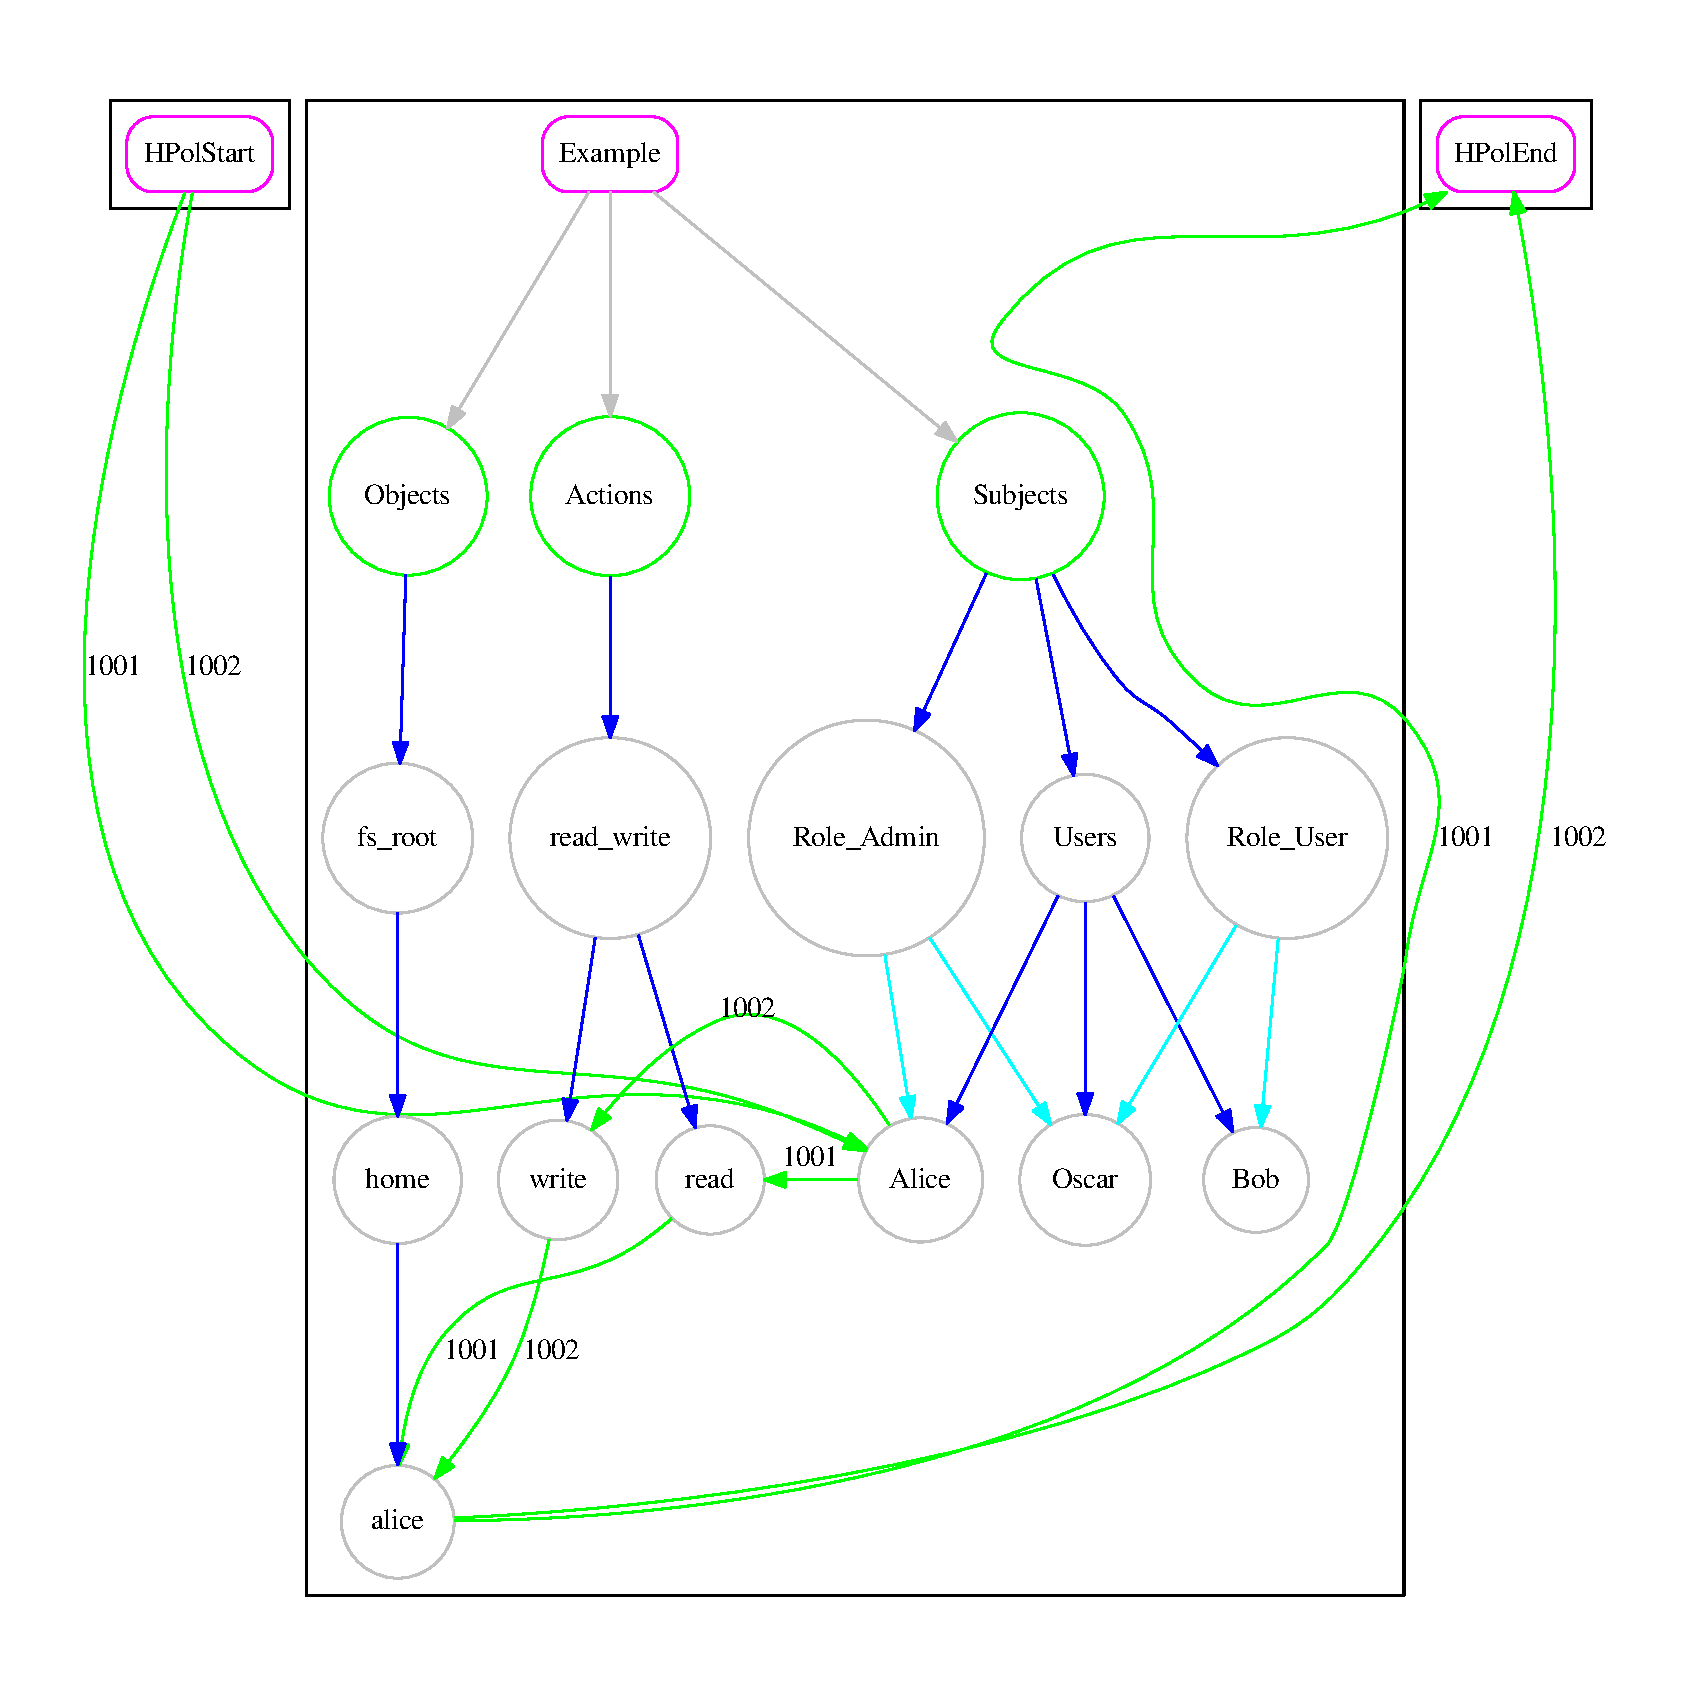
\includegraphics[width=\textwidth]{NewSELinux-AliceDirReadWrite.pdf}%%
\caption[File System Permission Example]{A file system permission example HPol model. This model contains three different users, two permission types and a single directory.}%%
\label{SELinuxAliceDirExample}%%
\end {figure}%%

\label{Section:FormalPolicyAbstraction}

One of the primary advantages of the \ac{hpol} approach to modeling security policies is that it sorts hierarchical organizational structures into their corresponding graph hierarchies through the use of Directed Acyclic Graphs (DAGs).

This approach enables the model to formalize these organizational hierarchies and define formal policy abstraction operations. For example, given the permissions of a file system, if a user has \node{write} permissions on all the files within a given sub-directory and the same user has \node{read} permissions on the same files, then it can be inferred that the user has both \node{read and write} permissions on all files in the subdirectory. If there are two separate policies allowing the \texttt{read} and \texttt{write} permissions on a file, then an abstraction can be made from these policies into a single policy that allows both reading and writing on the file. The \ac{hpol} model enables a straightforward and formal method for discovering these types of abstractions. In this example, a DAG would be created to represent the file permissions hierarchy. Then in such a DAG a \node{read\_write} node would be the parent node of nodes \node{read} and \node{write}, hence allowing the abstraction to be inferred and represented by the formal \ac{hpol} model.


Figure {\ref{SELinuxAliceDirExample}} shows a graph representation of the example described above. Observe that in the figure, there are two paths from the \node{HPolStart} node to the \node{HPolEnd} node; both paths are drawn with green arrows. The paths in figure \ref{SELinuxAliceDirExample} are described below in detail:

\begin{enumerate}
	%%
	\item%%
	{Path in which all the links are labeled with the \textit{1001} identifier composed of the following green arrow links:
		\begin{enumerate}
			\item%%
			Starting at the \node{HPolStart} node going to the \node{Alice} node in the \texttt{Subjects} DAG.
			\item%%
			Moving to the \node{read} node under the \texttt{Actions} DAG from the \node{Alice} (Subjects) node.
			\item%%
			Moving to the \node{alice} node under the \texttt{Objects} DAG from the \node{read} (Actions) node.
			\item%%
			Ending at the \node{HPolEnd} node coming from the \node{alice} (Objects) node.
		\end{enumerate}
	}%%
	%%
	\item%%
	{Path in which all the links are labeled with the \textit{1002} identifier composed of the following green arrow links:
		\begin{enumerate}
			\item%%
			Starting at the \node{HPolStart} node going to the \node{Alice} node in the \texttt{Subjects} DAG.
			\item%%
			Moving to the \node{write} node under the \texttt{Actions} DAG from the \node{Alice} (Subjects) node.
			\item%%
			Moving to the \node{alice} node under the \texttt{Objects} DAG from the \node{write} (Actions) node.
			\item%%
			Ending at the \node{HPolEnd} node coming from the \node{alice} (Objects) node.
		\end{enumerate}
	}%%
\end{enumerate}

Note that the only difference between these two policy paths is the \node{read} node in the first path (1001) as a file permission and the \node{write} node in the second path (1002) as a file permission. Also note that the same subject node, \node{Alice}, and the same object node, the \node{alice} home directory node, are equal in both policy paths.

With this formalization of a policy using policy paths plus the fact that the permissions are organized in a hierarchical manner, the information and inference rules needed to make the abstraction are all present. The information needed to make this abstraction is given by the policy paths and the hierarchy in the DAGs; in this case, the permissions DAG in which the \node{read\_write} node is the parent of the \node{read} and \node{write} nodes. 

{The two policy paths described above could be abstracted by one unique hypothetical policy path as follows:}

\begin{enumerate}
	%%
	\item%%
	{Path in which all the links would be labeled with the \textit{1001-1002} identifier composed of the following links:
		\begin{enumerate}
			\item%%
			Starting at the \node{HPolStart} node going to the \node{Alice} node in the \texttt{Subjects} DAG.
			\item%%
			Moving to the \node{read\_write} node under the \texttt{Actions} DAG from the \node{Alice} (Subjects) node.
			\item%%
			Moving to the \node{alice} node under the \texttt{Objects} DAG from the \node{read\_write} (Actions) node.
			\item%%
			Ending at the \node{HPolEnd} node coming from the \node{alice} (Objects) node.
		\end{enumerate}
	}%%
	%%
\end{enumerate}


This type of policy abstraction operation would also be applicable to other areas of policy DAGs. A similar abstraction could be made in the subject DAG of figure \ref{SELinuxAliceDirExample}. Suppose the user \node{Oscar} had a similar read-write policy that \node{Alice} has with the only difference being the subject of the policy, \node{Oscar} instead of \node{Alice}. Also, note that both Oscar and Alice are secondary children of the \node{Role\_Admin} node. With the combination of the similar policy paths and the common parent of both the \node{Oscar} and \node{Alice} node, an abstraction policy could be formed that states that the Admin Role has the permission to read and write on the \texttt{alice} directory. Also, note that this abstraction cannot be applied to the \node{Users} node. This is because the \node{Bob} node would not have this policy. Only when all of the children of a parent node have a similar policy can a full abstraction be made. Abstractions in the opposite direction are possible as well. If a policy states that the Admin Role can \texttt{read} and \texttt{write} on the \texttt{alice} directory then it can be inferred that all children of the \node{Role\_Admin} node also have the ability to \texttt{read} and \texttt{write} on the \texttt{alice} directory.

Our goal is to allow the model and its computational implementation to represent the low-level policy paths and to be able to represent and infer the high-level abstract policies. This would enable security policy analysis to choose the level of abstraction to visualize and verify the security policies within and across a system.

\section{The HERMES Language}
\label{Section:Hermes}
%move current to The Hpol Formal Model chapter once edited
%or move to background with The HPol Formal Model

%\acf{hermes}, is a language which allows IT security personnel to describe their organization's infrastructural knowledge and security policies, using the following four entity sets: Domains/Devices, Groups of Users and Roles, Applications, and Actions (hereby referred to as ``entity sets"). Each of the entity sets can be defined using a hierarchical structure. Policies are specified in the form of elements applied to a given combination of entity sets. The uniqueness of HERMES lies in following four features:

\acf{hermes}, is a specification language that allows cyber security personnel to describe an organization or industry's infrastructure security policies using entity sets. Each entity set can classify a variety of components such as Domains, Groups of Users, Roles, Application and so on. \ac{hermes} allows entity sets to be defined using a hierarchical structure. Because of this structure, an \ac{hpol} model can be represented as a series of entity sets. The flexibility and uniqueness of \ac{hermes} lies in the following features:

%\paragraph{Platform Independent} HERMES is a text-based language capable of specifying security policies for any kind of application, on any platform and in any type of organization. HERMES is designed to be flexible enough to be able to specify any kind of policy with respect to any piece of infrastructure, operating in any kind of environment. Such flexibility and platform in-dependency enables easier use of source code management tools, available to system developers. Tools that many IT personnel and system administrators have began to use in a process commonly called as ``DevOps".

\paragraph{Platform Independent:} \ac{hermes} is a text-based language interpreted by a Prolog engine. Because Prolog is platform independent, \ac{hermes} is as well. Also, \ac{hermes} is capable of specifying security policies for any kind of application, on any platform or operating system and in any context. This is because all parameters of a \ac{hermes} entity set are flexible. There are no keywords required to define entity sets. All a system administrator would have to do is follow the very simple syntax defined by \ac{hermes}. 

%\paragraph{Human-Centered and Ease of Use} HERMES is designed to be directly used (written and read) by humans rather than computers. HERMES is similar to YAML, but it is not based on XML or other similar verbose markup languages. XML-based languages are suitable for machine-to-machine communication but not for communication amongst humans. HERMES' design encourages its usage as a tool for organizational policy discussion and exchange between different groups, different corporations, and different associations of professionals.

\paragraph{Human-Centered and Ease of Use:} \ac{hermes} is designed to be written and read by humans, not computers. \ac{hermes} is similar to YAML, but is not based on XML or any other similar verbose markup languages. XML-based languages are difficult and obscure to read and write for humans. \ac{hermes} is designed to be easy to read and write by humans. Listing \ref{list:PolicyHERMES} contains an entity set written in \ac{hermes}. As shown \ac{hermes} entries are written using words and very little special characters when compared to other specification languages such as XML.

\begin{lstlisting}%%
[
label={list:PolicyHERMES}, 
caption={Example of HERMES usage (to disable Javascript in all web browsers for all machines connected to a server).\cite{hifipolbro}\cite{Jillepali1}}, 
keepspaces=true,
style=hermes,
float
]
Policy: ID_001
{
	Description: "Disabling JavaScript.";
	Rationale: "Security Vulnerability";
	Status: "Enabled";
	Field: (JavaScript, "Disabled");
	ApplyTo: "ALL";
}
\end{lstlisting}

%\paragraph{Versatile Specification Capacity} HERMES enables the native specification of organization's infrastructural knowledge in a hierarchical manner. For example, an organization can be specified by its name and it's Marketing department can be specified as a child. Using HERMES, a tree or graph structure can be defined for any of the entity sets, at any desired level of granularity, since organizations are well accustomed to using tree-like organizational hierarchies. HERMES enables the specification of security policies at any desired level of granularity and/or specificity, within the organization's infrastructural knowledge. Using HERMES, a policy designer can specify that a given action or prohibition may apply to any Cartesian combination of users and client machines sets respectively, within an organization. 

\paragraph{Versitile Specification Capacity:} \ac{hermes} allows the specification of an organization's infrastructure in a hierarchical manner. For example, a company's organizational chart can be specified in \ac{hermes} with the top most entity set being the CEO and the next level of branches being the children of this entity set, such as the marketing and IT departments. \ac{hermes} can easily define tree and graph structures through its entity sets. It is because of this that \ac{hermes} was chosen to represent \ac{hpol} formal models. Its parameterized nature and its ease of use make it ideal for use in both an IT environment and in the \ac{hpol} framework.

%\paragraph{Instantiation} HERMES is designed to accommodate the automatic generation of configurations for respective infrastructure items, based on the high-level policy specification. There is a project which aims to use HERMES for specifying security policies for web browsers and transform the policies into configurations. The project is called HiFiPol:Browser. The architecture of this system has been described in \cite{hifipolbro}.

\ac{hermes} is designed to accommodate the automatic generation of entity sets based on high-level policy specifications. Because of this \ac{hermes} was chosen to be an intermediate language for the \ac{hpol} framework. \ac{hermes} was originally used for the specification of security policies in web-browsers. This project is called HiFiPol:Browser \cite{hifipolbro}\cite{Jillepali1}. \ac{hermes} was then later adapted for use in the \ac{hpol} project.


\chapter{Formal Router Policy Modeling}
\label{Chapter:CiscoRouterPolicyModeling}

In this chapter, formal modeling of a Cisco Site-to-Site VPN policy with the \ac{hpol} model is described. Two complete router configurations will be modeled in this chapter. A policy will also be traced through the resulting \ac{hpol} formal model graph to demonstrate the models effectiveness.

\begin{figure}
	\centering
	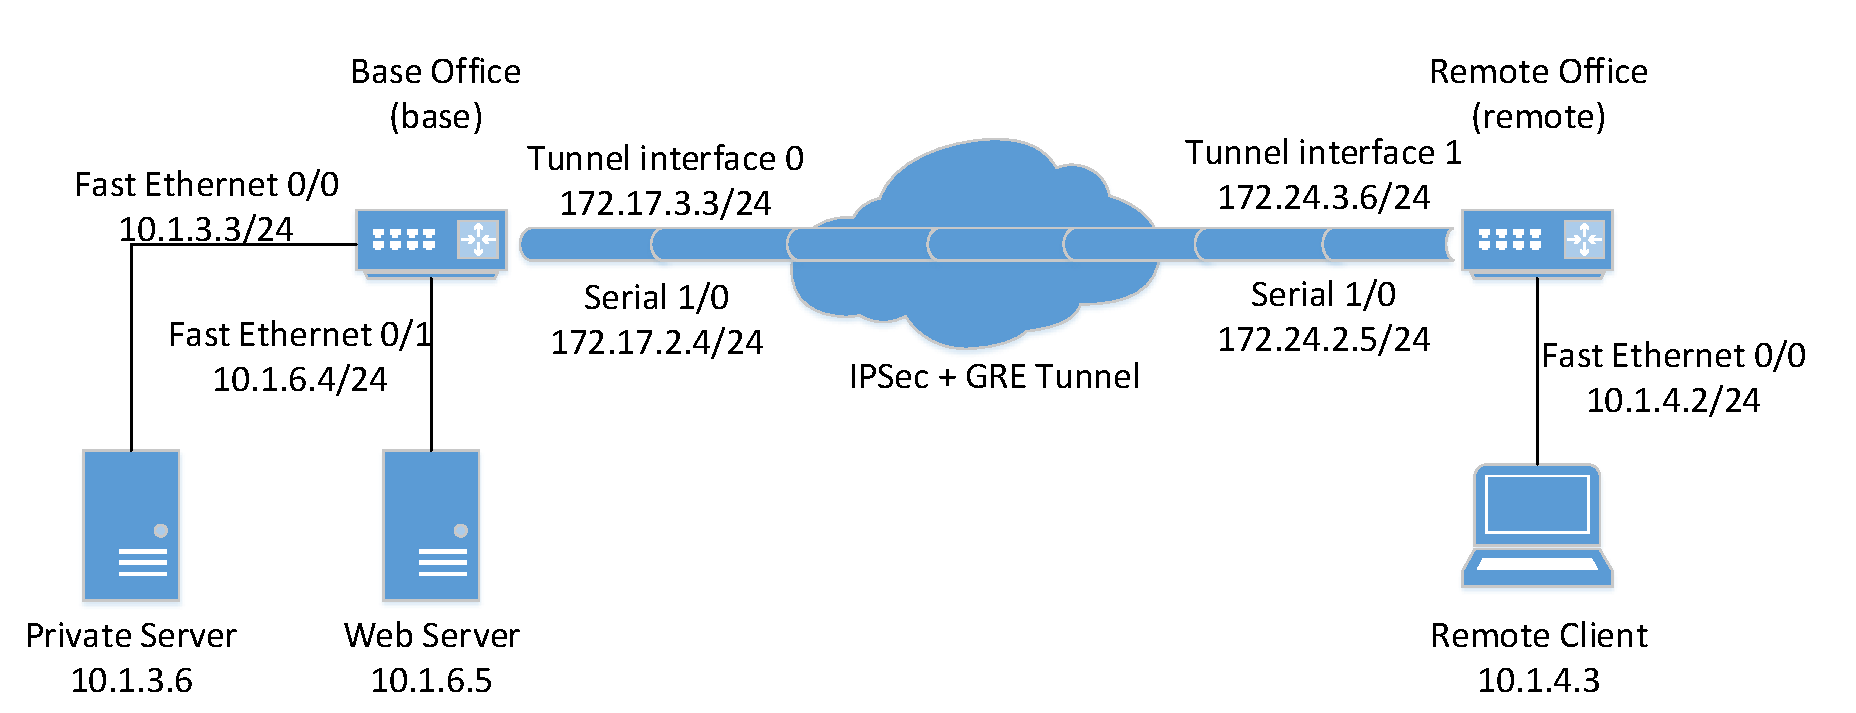
\includegraphics[width=\textwidth]{hpolVPNexample.pdf}
	\caption{Site-to-Site VPN Scenario (based on {\cite{CiscoVPNExampleWebLink}}).}%%
	\label{CiscoVPNExample}%%
\end{figure}%%

\section {Cisco Site-to-Site VPN Policy}
\label{Chapter:ExemplarCiscoVPN}

{The scenario which is parsed and modeled was developed by Cisco for training purposes and is described in detail on the Cisco site-to-site VPN training website {\cite{CiscoVPNExampleWebLink}}. Figure {\ref{CiscoVPNExample}} shows a similar network architecture for this site-to-site VPN example and corresponds to Figure 3-8 in the Cisco example which is available in the online Cisco example.}

{In the example presented in Figure {\ref{CiscoVPNExample}} the following can be observed:}

\begin{enumerate}
	%%
	\item%%
	{VPN: There are two routers, left, hq-sanjose and right, ro-rtp, connected by an encrypted VPN tunnel.}
	%%
	\item%%
	{LAN(s) Left: The left router has two internal VLANs, DMZ and private, which are connected to it with assigned IPv4 addresses: 10.1.6.0/24 and 10.1.3.0/24, respectively.}
	%%
	\item%%
	{LAN(s) Right: The right router has one internal VLANs which is connected to it with assigned IPv4 addresses: 10.1.4.0/24.}
	%%
	\item%%
	{WAN: The left side of the tunnel has been assigned the IPv4 address of 172.17.2.4; the right side of the tunnel has been assigned the IPv4 address of 172.24.2.5. These are mapped to a serial interface in each router.}
	%%
	\item%%
	{Tunnel: The IPv4 addresses assigned to the tunnel are 172.17.3.3 and 172.24.3.6 for the left and right routers respectively. These are mapped to a tunnel interface in each router. These two interfaces are virtual interfaces. The tunnel's encapsulation protocol is GRE+IPSec.}
	%%
	\item%%
	{Host: A public Web server in the DMZ VLAN has been assigned the 10.1.6.5 IPv4 address.}
	%%
	\item%%
	{Host: A private server in the internal (left) VLAN has been assigned the 10.1.3.6 IPv4 address.}
	%%
	\item%%
	{Host: A private client in the internal (right) VLAN has been assigned the 10.1.4.3 IPv4 address.}
	%%
	\item%%
	{Note: As indicated by the last two entries, the external IPv4 addresses assigned to the two routers are actually non-usable reserved IPv4 addresses used only as an example. A production configuration will configure here instead actual usable external IPv4 addresses.}
	%%
	\item%%
	{Note: In this case both of the routers would be configured to perform Network Address Translation (NAT) between the external and the internal VLANs.}
	%%
\end{enumerate}

\section{The Path of a Packet in the Example VPN Tunnel}

{In order to validate that our \ac{hpol} model and tool-set are accurately modeling the routing policy established by the VPN Tunnel example described in the previous section, the steps followed by an IP packet in the given site-to-site VPN configuration will be manually traced. Section \ref{Section:HPolPacketTrace} will show how the \ac{hpol} formal model also models the same forwarding and security policy.}

\begin{enumerate}
	%%
	\item%%
	{Let's assume that a user in PC A, IPv4 10.1.4.3, (right side of figure {\ref{CiscoVPNExample}}) is accessing services provided by the private corporate server at 10.1.3.6 through the Site-to-Site VPN Tunnel.}
	%%
	%%
	\item%%
	{A given IP packet would be initiated at the PC A client, IPv4 address 10.1.4.3, and sent to the gateway at the router endpoint of IPv4 address 10.1.4.2, which is within the same subnet and VLAN.}
	%%
	\item%%
	{The \textit{ro-rtp} router (right) would then see that the packet has a destination IPv4 address of 10.1.3.6 corresponding to the private corporate server on the other side of the VPN tunnel. Hence, the router would encapsulate the packet using the VPN tunnel logical addresses: source, IPv4 172.24.3.6, and destination, IPv4 172.17.3.3, and send it through the tunnel interface, IPv4 172.24.2.5. In order to accomplish this, multiple encryption and encapsulation steps would need to be carried out by the router given the router configuration. These steps are described in the next subsection.}
	%%
	\item%%
	{When receiving the packet on its tunnel serial interface, IPv4 172.17.2.4, the \textit{hq-sanjose} router (left) would then unwind the tunneling and encryption steps performed by the \textit{ro-rtp} router.}
	%%
	%%
	\item%%
	{Lastly, the packet whose source IPv4 address is 10.1.4.3 and whose destination IPv4 address is 10.1.3.6 would be send via the Private VLAN to the Private corporate server from the gateway interface, IPv4 10.1.3.3.}
	%%
\end{enumerate}

%% \section{The Example Cisco Router Configuration File}

%% {In this section we will describe in detail the encryption and forwarding steps configured in each router and how the IOS policy configuration file describes such forwarding and security policy implementation.}


\begin{figure*}
\centering

%\sbox0{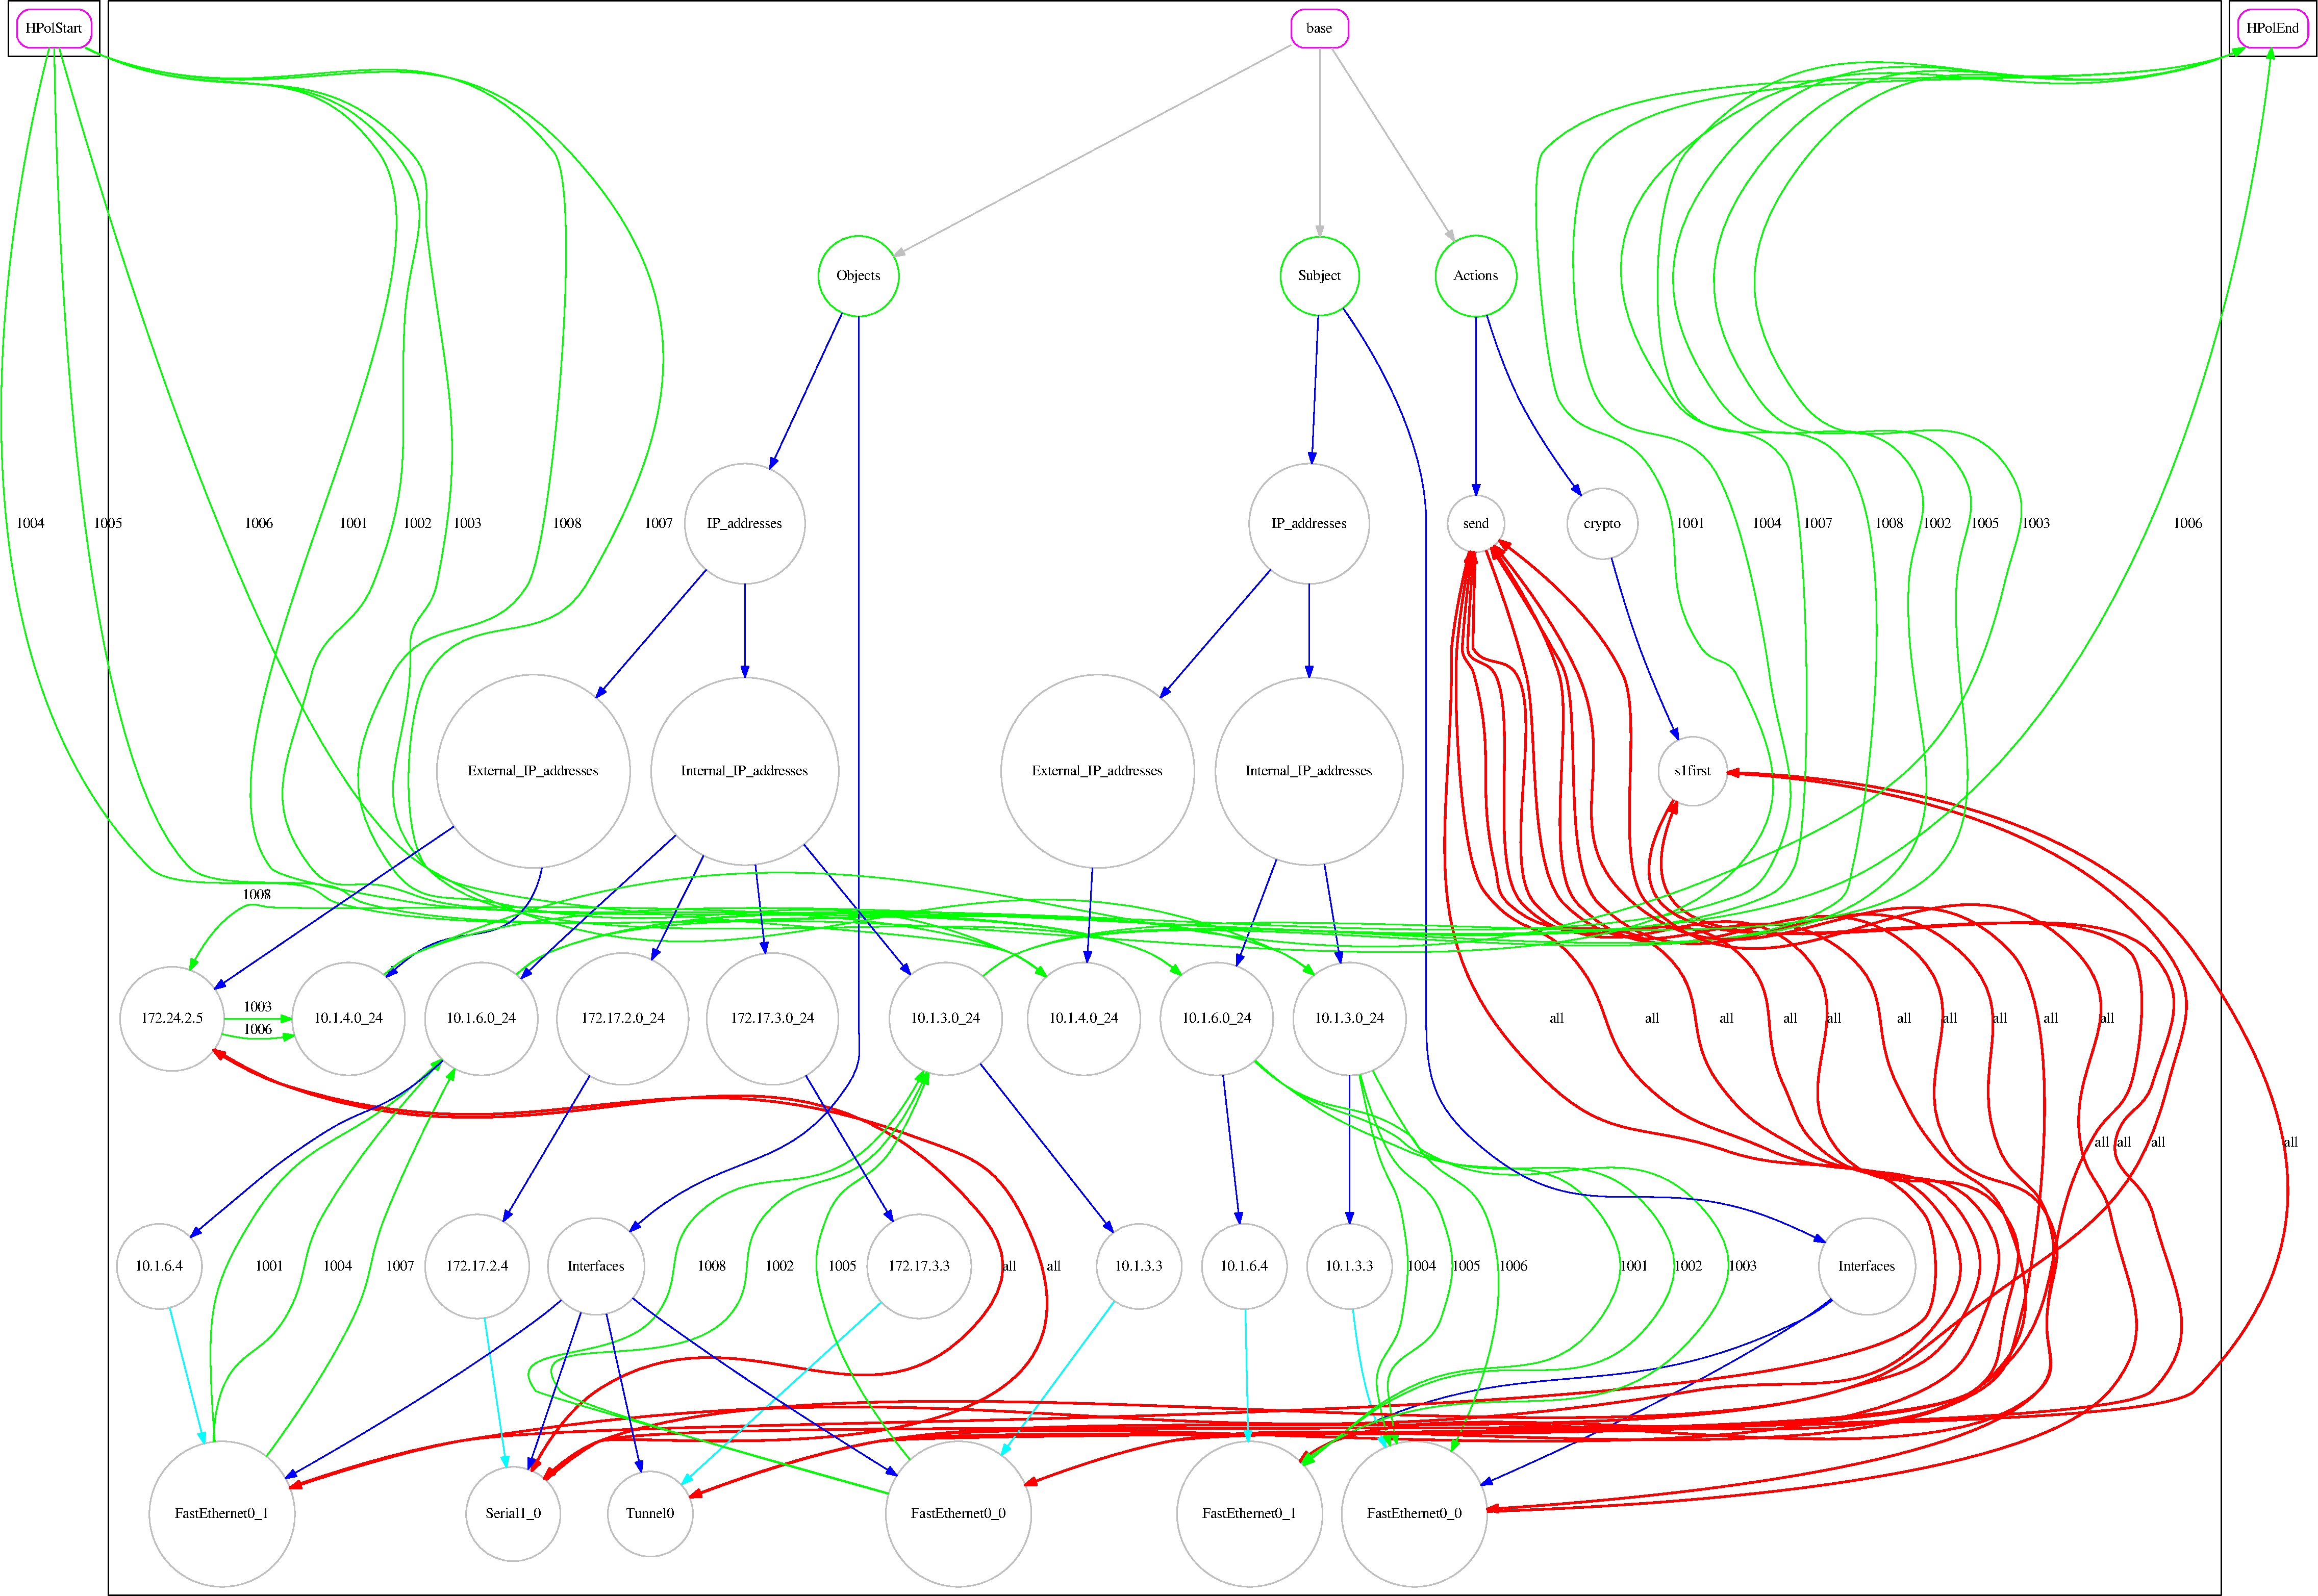
\includegraphics{s2svpnA}}
%\begin{adjustbox}{rotate=90, center}
%	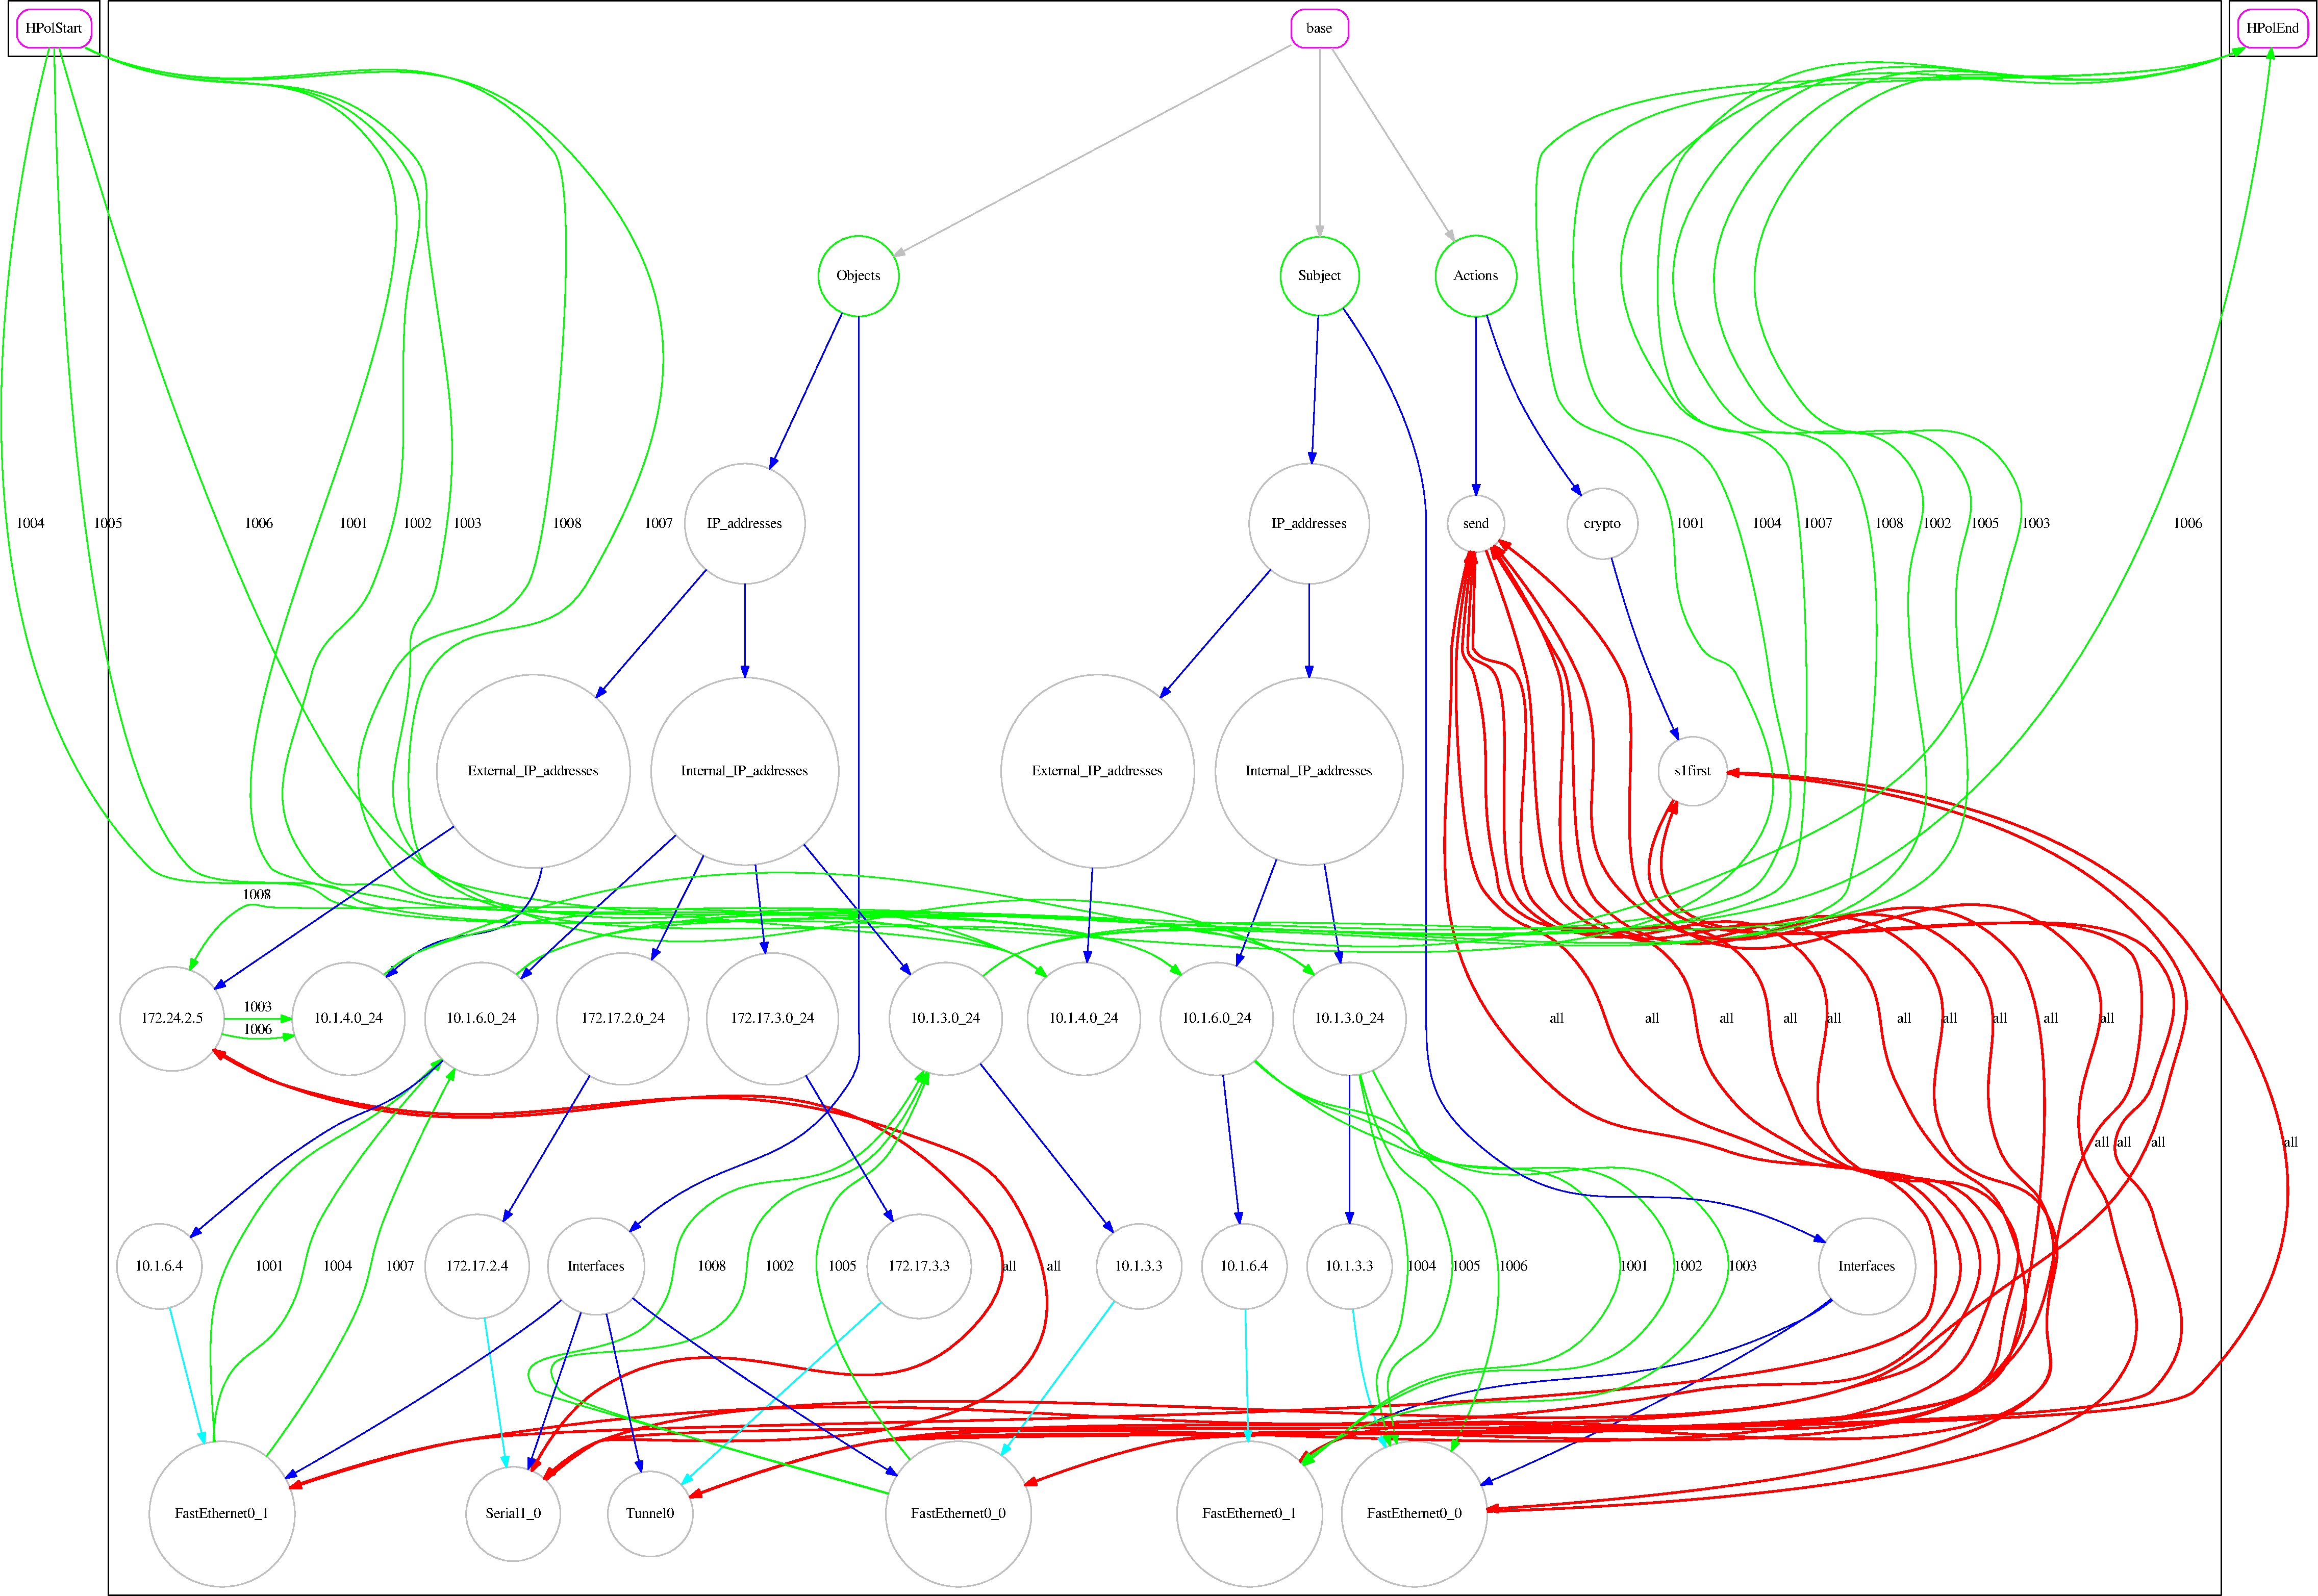
\includegraphics[clip,trim=0 0 0 {.5\ht0}, height=\textwidth, width=.45\textheight]{s2svpnA.pdf}
%\end{adjustbox}
%\begin{adjustbox}{rotate=90,center}%
%	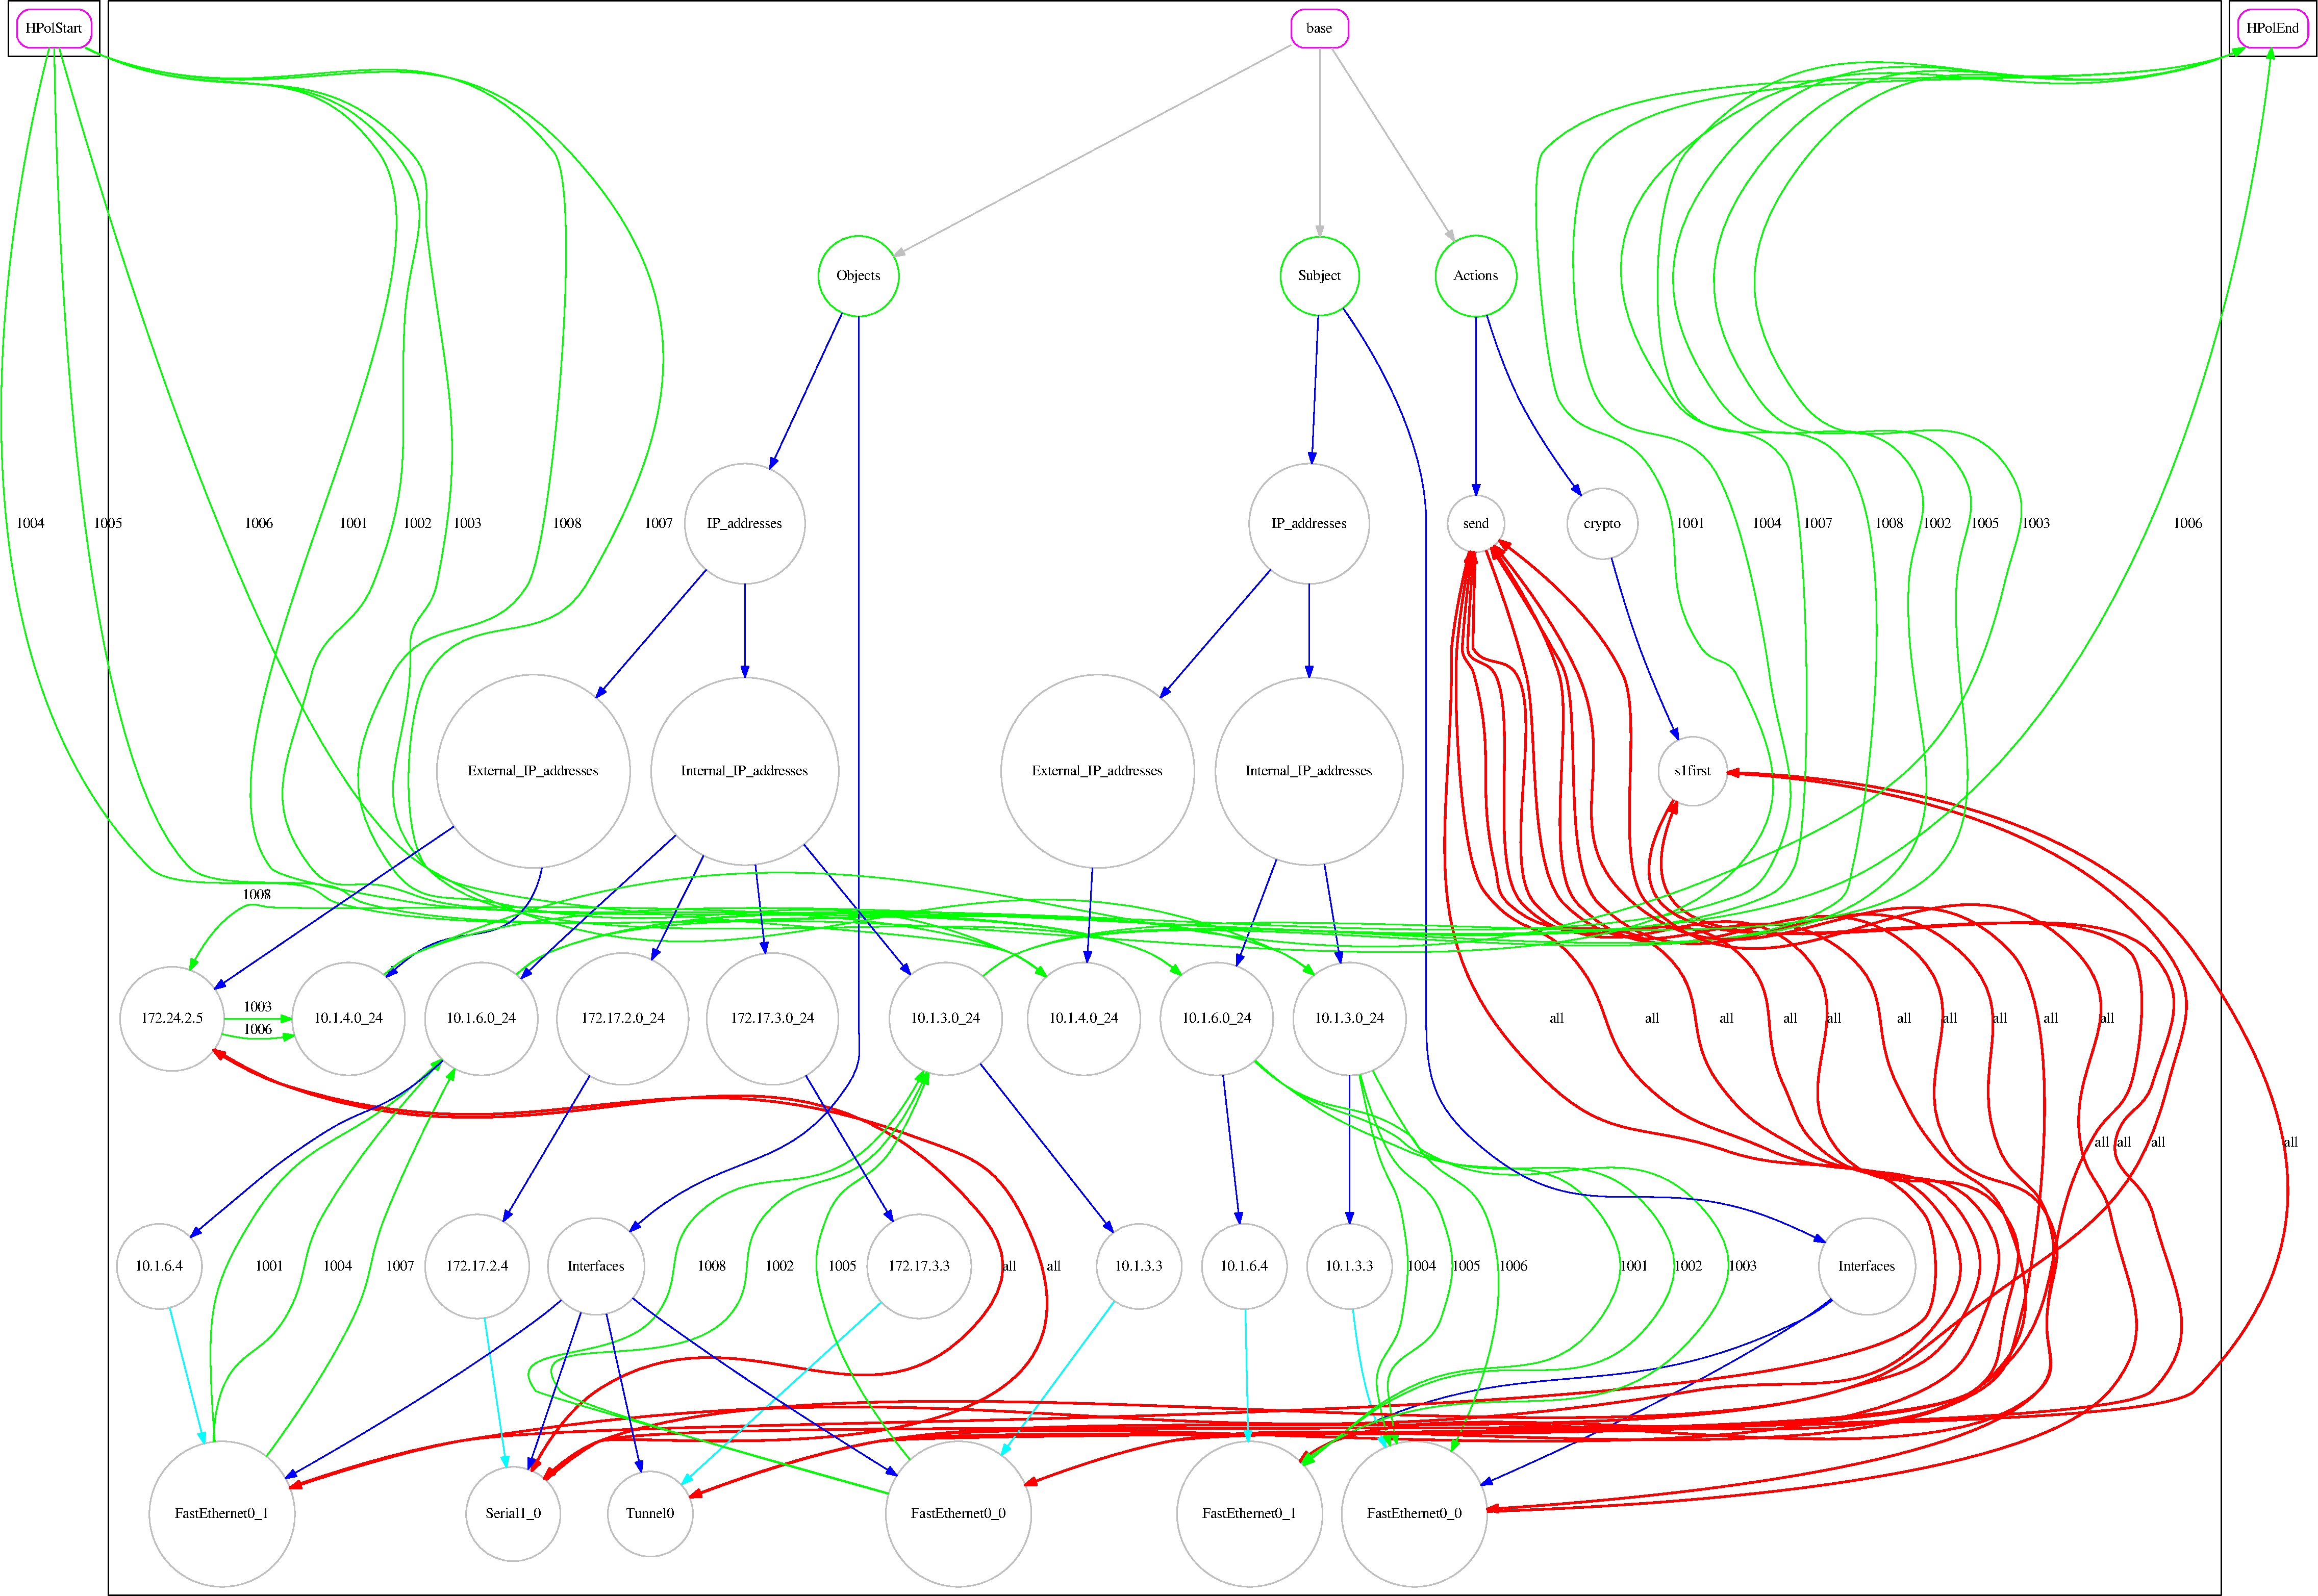
\includegraphics[clip,trim=0 {.5\ht0} 0 0, height=\textwidth, width=.45\textheight]{s2svpnA.pdf}
%\end{adjustbox}

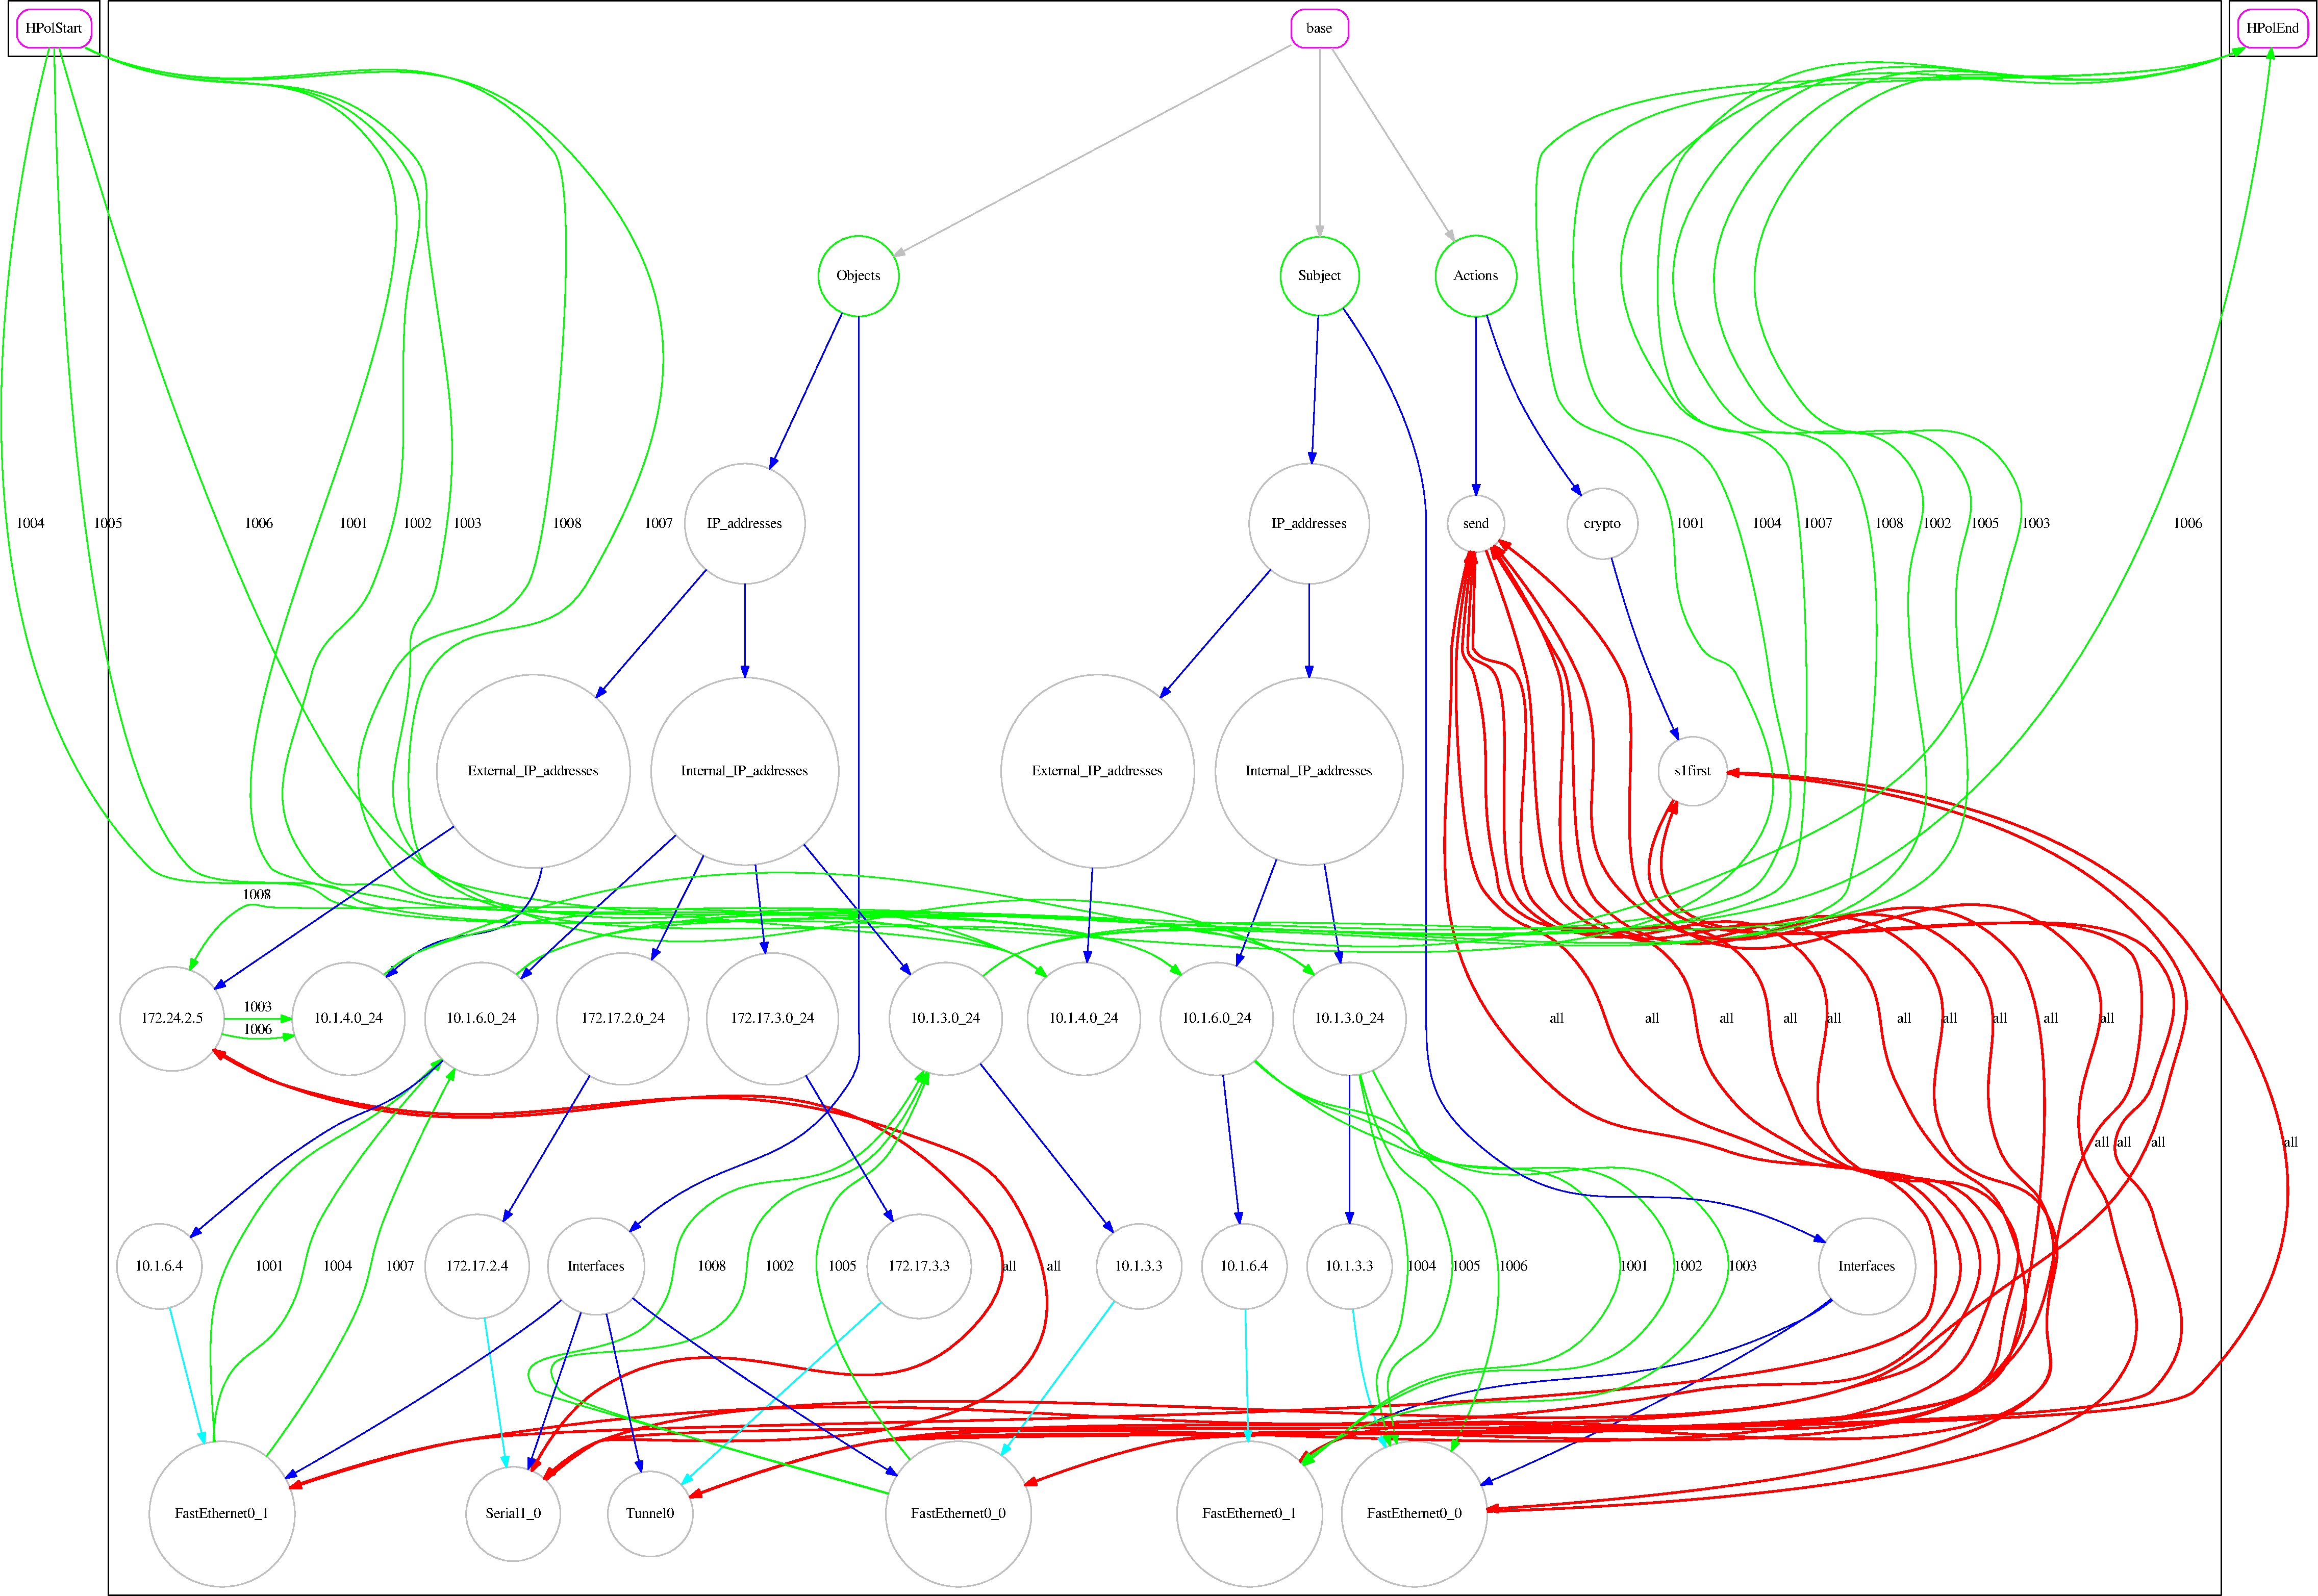
\includegraphics[angle=90, height=.9\textheight, width=\textwidth]{s2svpnA.pdf}

\caption{Cisco VPN HPol model: Graph View for Left Router, \textit{hq-sanjose}}%%
\label{CiscoRouterAGraph}%%
\end{figure*}


\begin{figure*}
\centering

%\sbox0{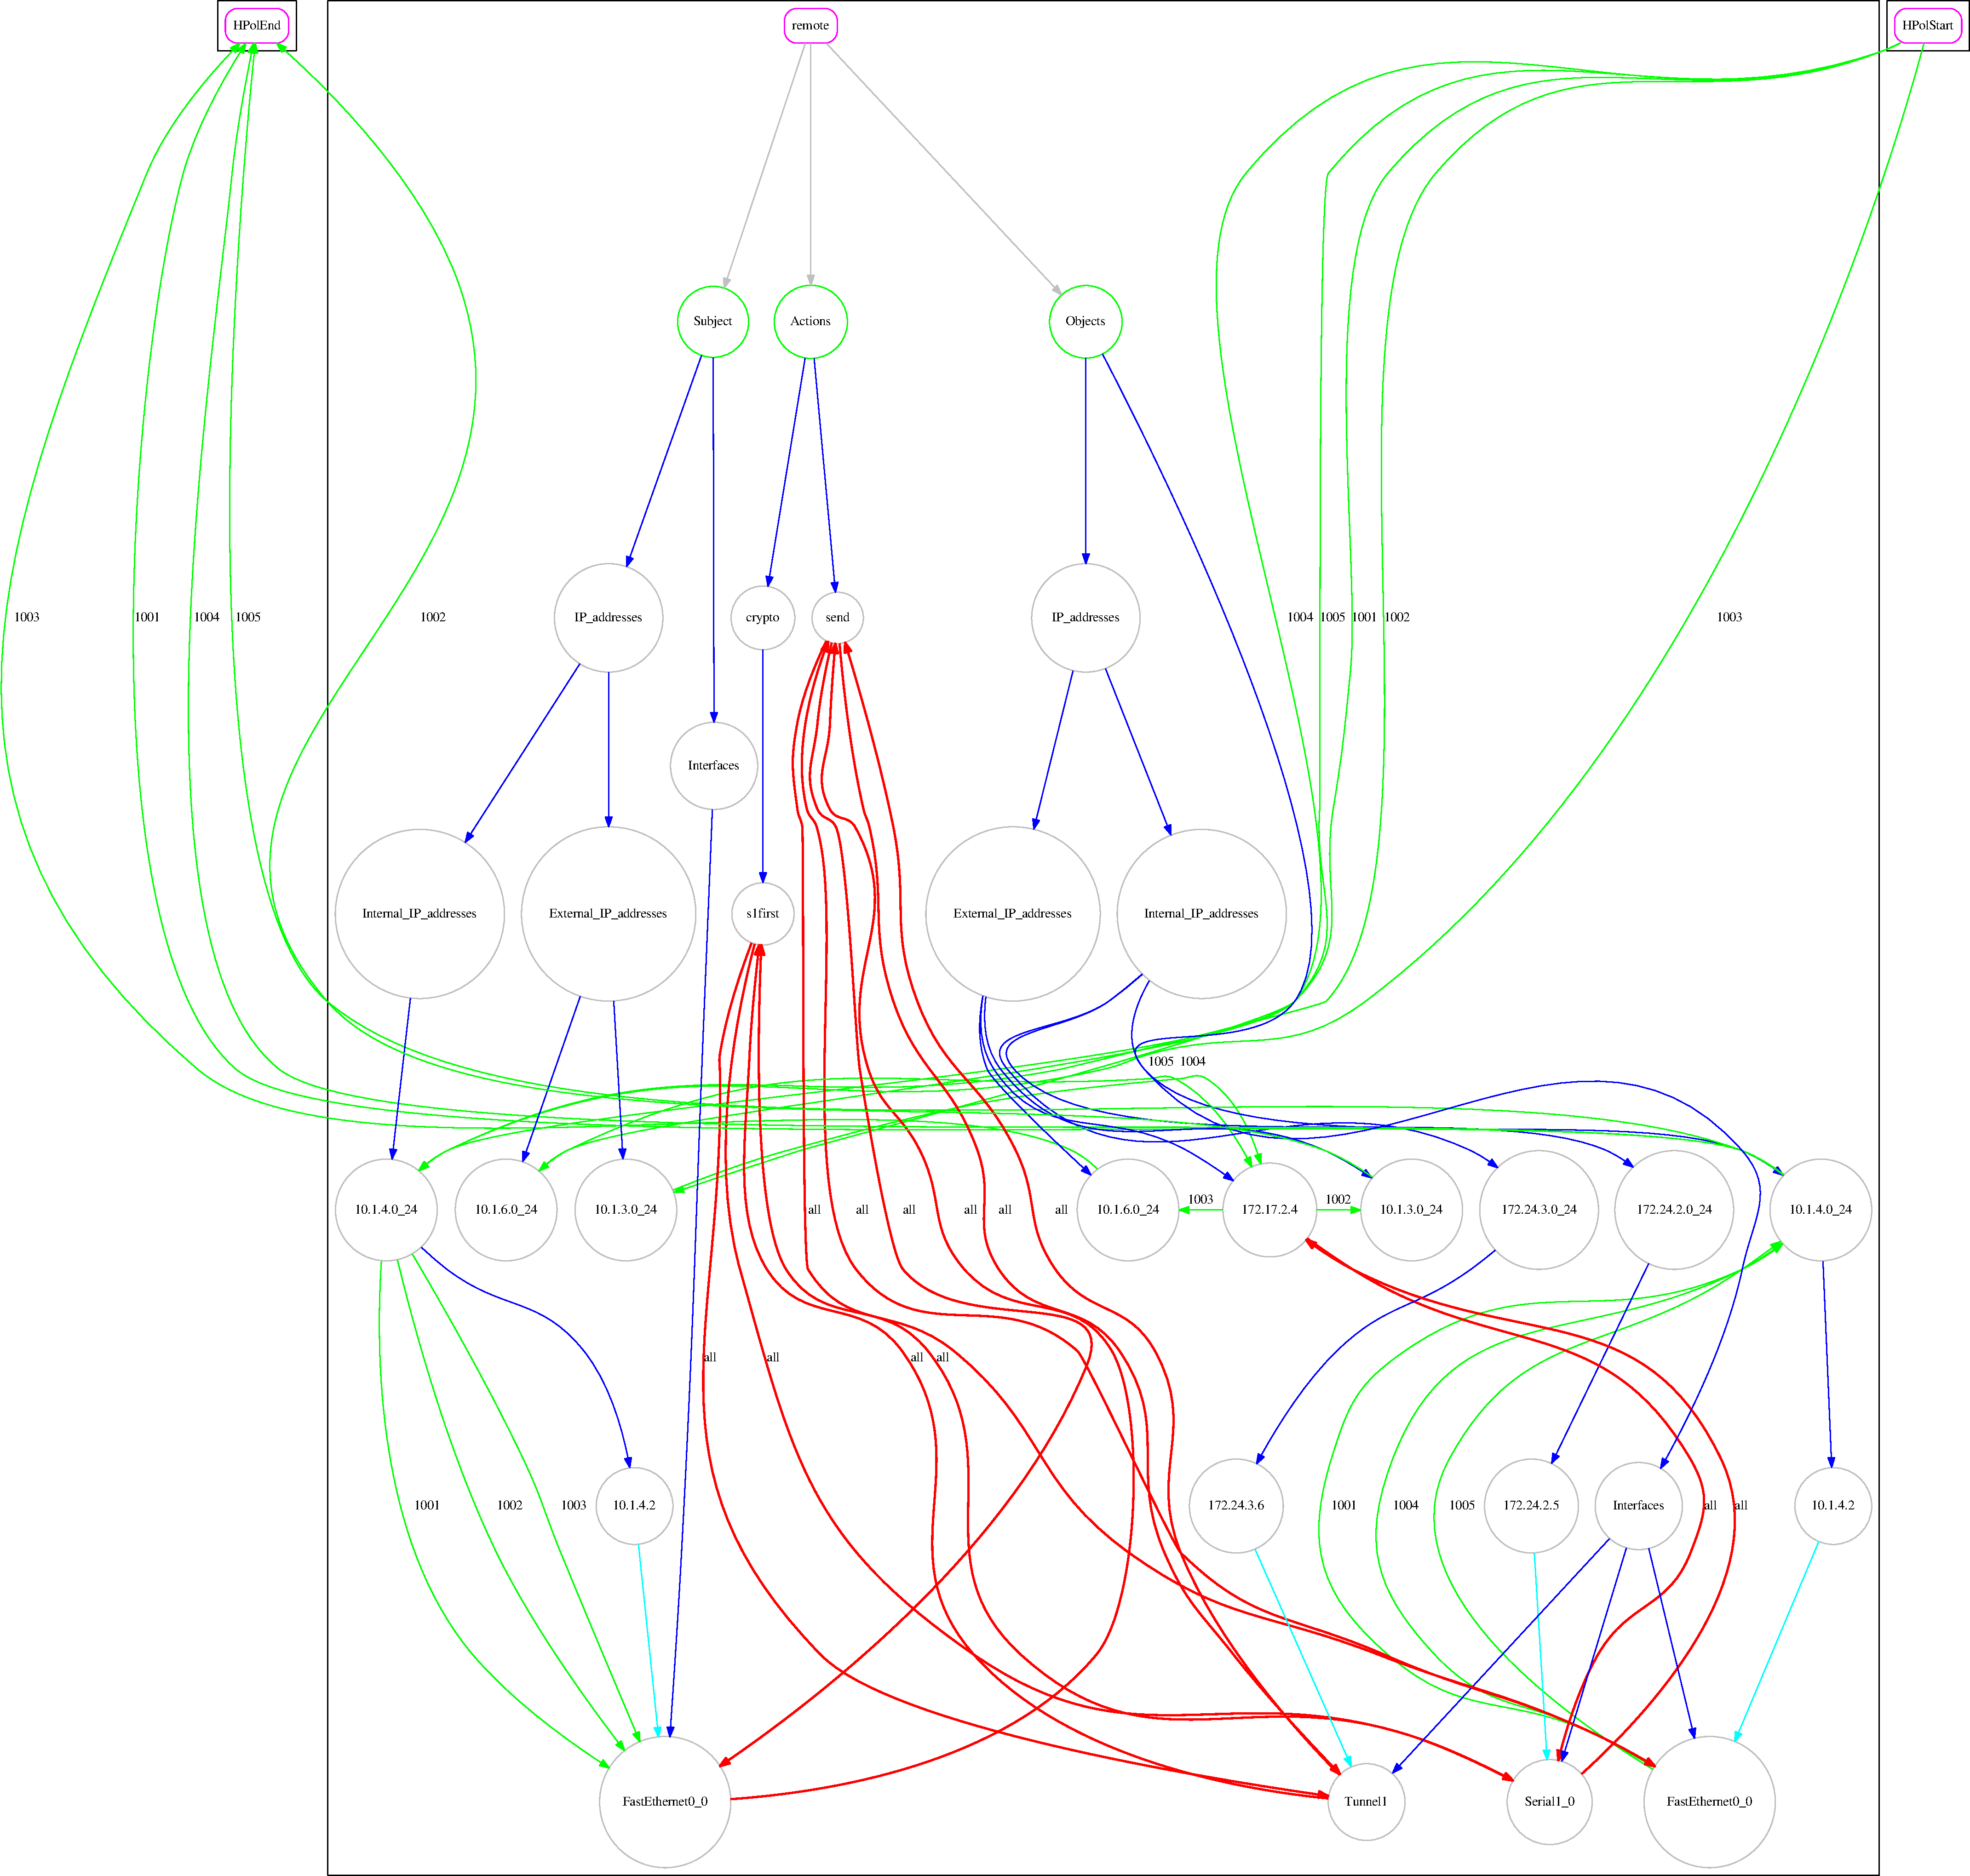
\includegraphics{s2svpnB}}
%\begin{adjustbox}{rotate=90, center}
%	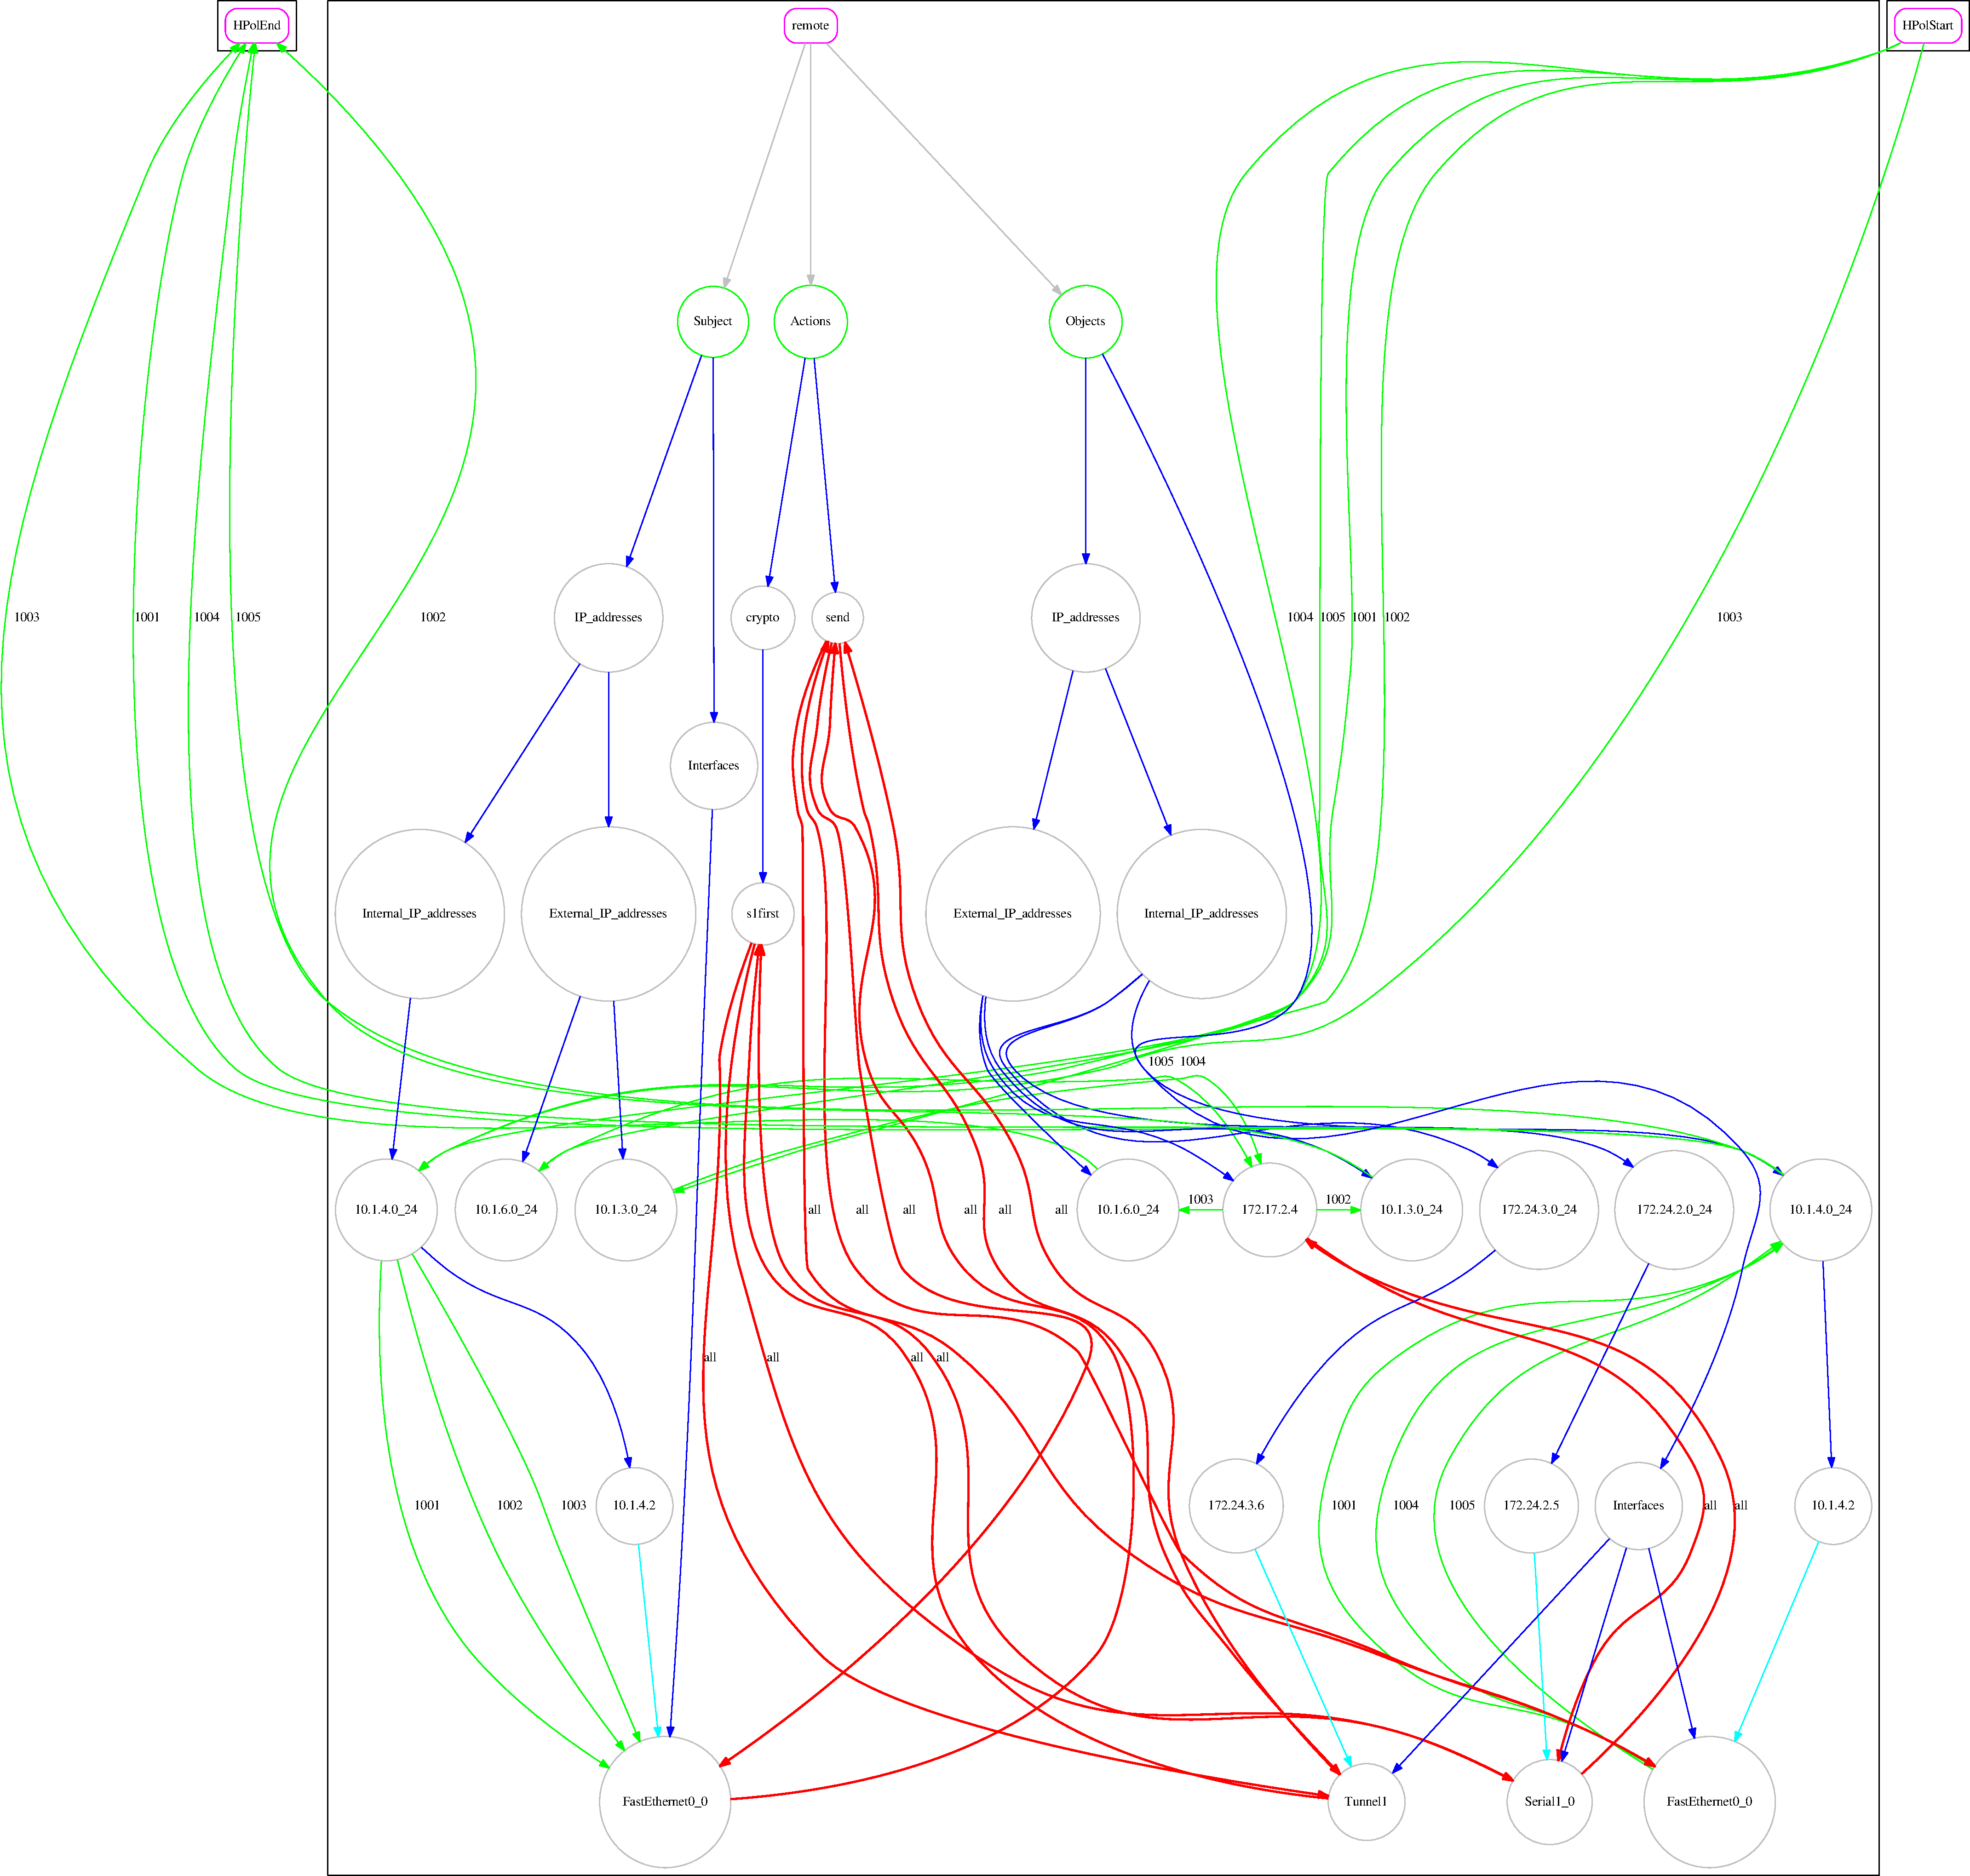
\includegraphics[clip,trim=0 0 0 {.5\ht0}, height=\textwidth, width=.45\textheight]{s2svpnB.pdf}
%\end{adjustbox}
%\begin{adjustbox}{rotate=90,center}
%	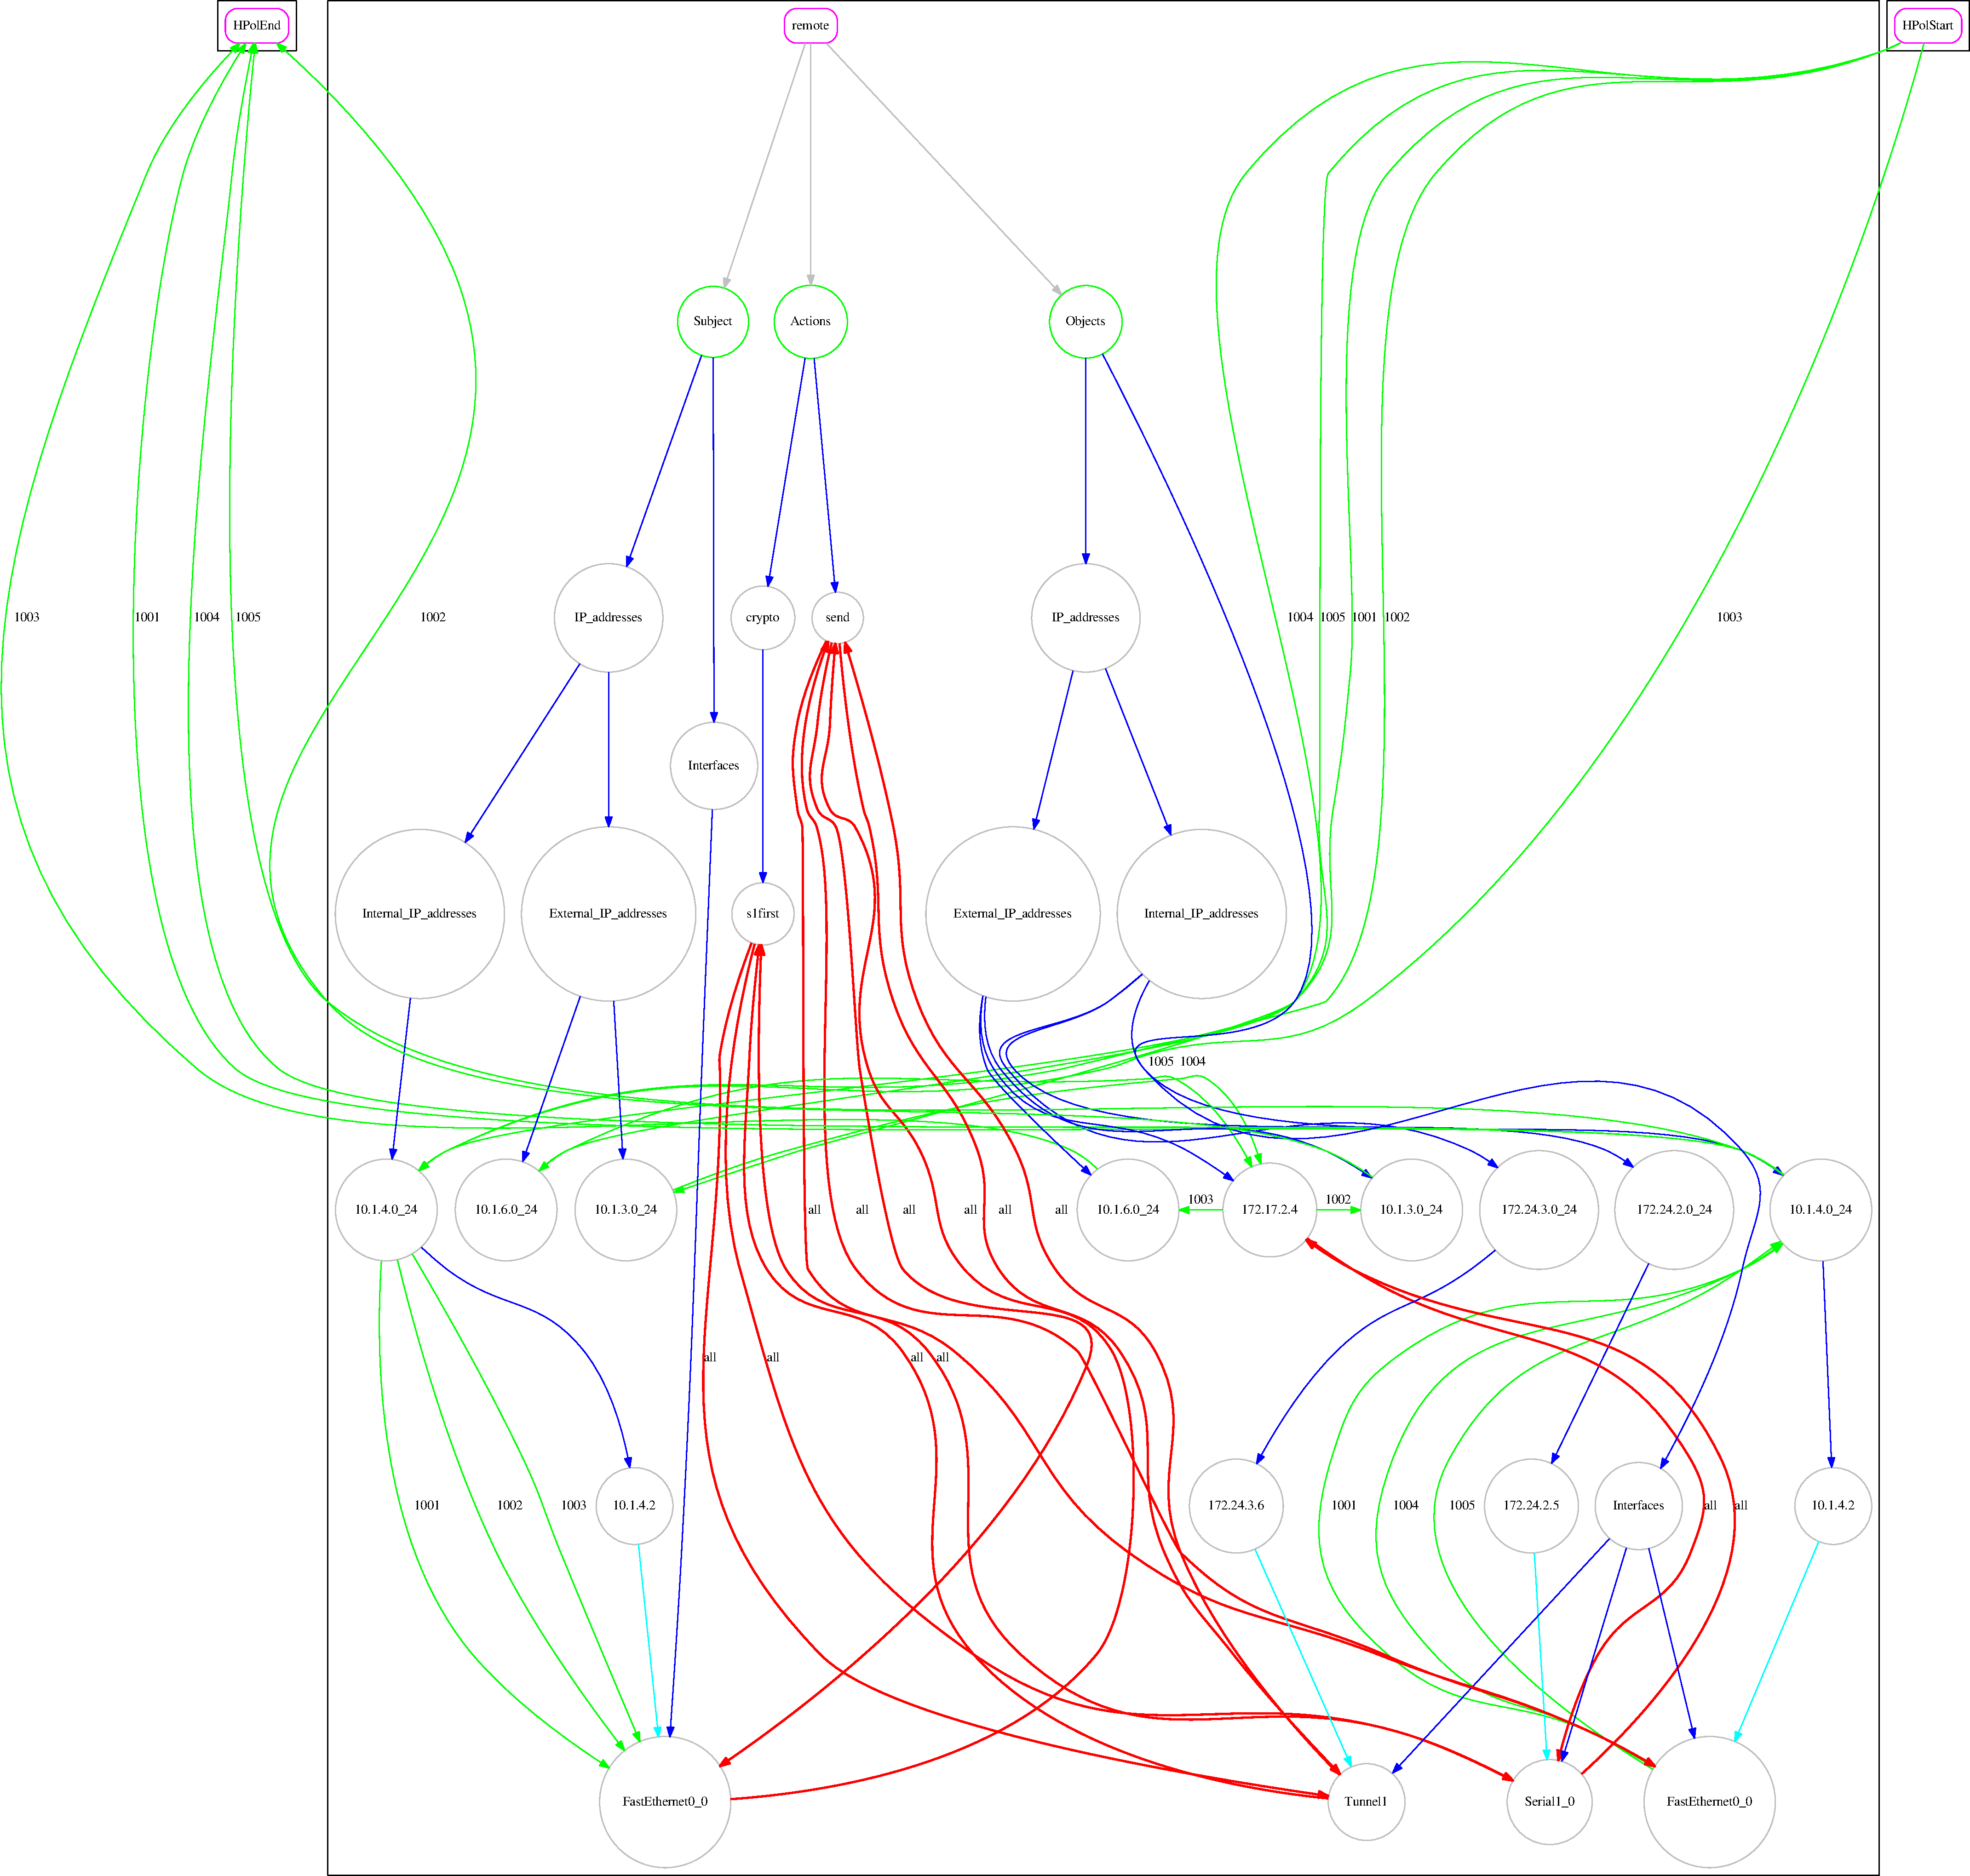
\includegraphics[clip,trim=0 {.5\ht0} 0 0, height=\textwidth, width=.45\textheight]{s2svpnB.pdf}
%\end{adjustbox}

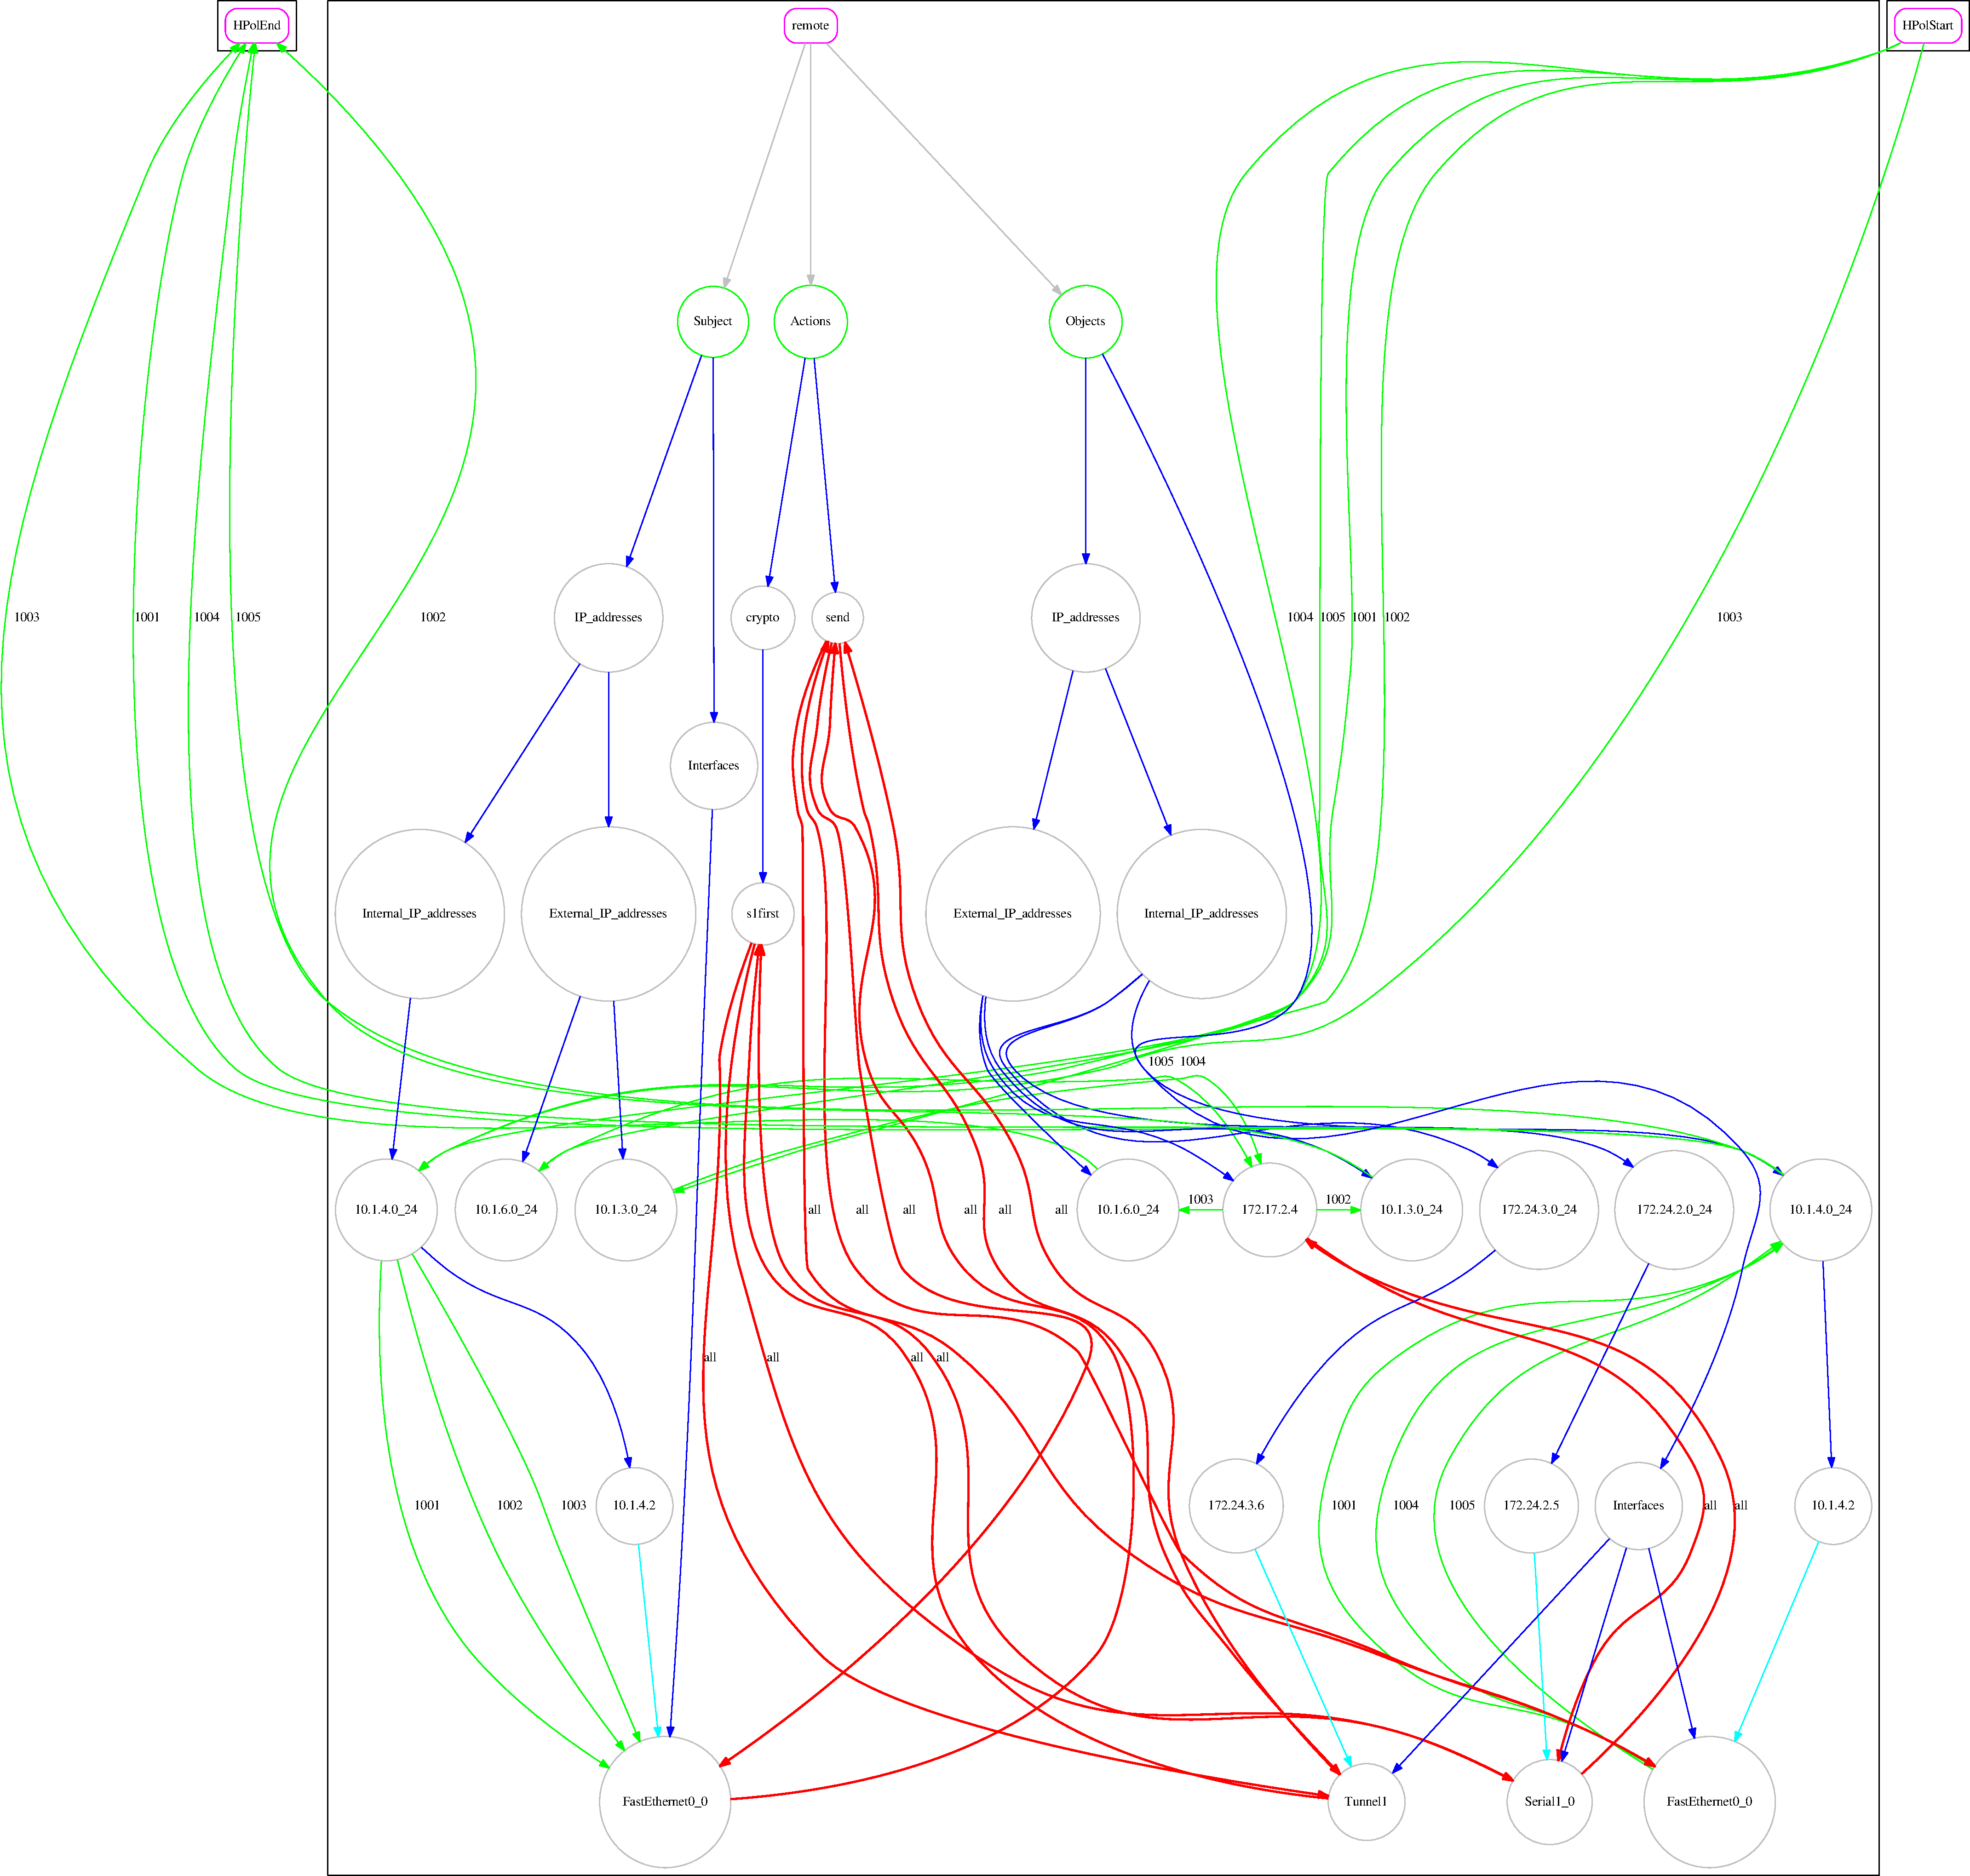
\includegraphics[angle=90, height=.9\textheight, width=\textwidth]{s2svpnB.pdf}

\caption{Cisco VPN HPol model: Graph View for Right Router, \textit{ro-rtp}}%%
\label{CiscoRouterBGraph}%%
\end{figure*}%%


\section{The Cisco Configuration Parser}
%add more 
%add some code PYTHON

{A parser was created in Python that reads a Cisco configuration file and by using the \ac{hpol} framework creates a graph representation of a router's policy. Figures \ref{CiscoRouterAGraph} and \ref{CiscoRouterBGraph} show the policy graphs resulting from this process. The configuration parsed for this example may be found on the Cisco site-to-site VPN training website {\cite{CiscoVPNExampleWebLink}}.}

{The generalized router HPol format is as follows:}
\begin{itemize}
	\item{Numbers above links represent a policy number.}
	\item{A link illustrates a step in the policy.}
	\item{Subnet nodes verify that a packet contains an acceptable source address.}
	\item{Interface nodes verify that a packet was received at a particular interface.}
	\item{Action nodes represent a transform that is applied to a packet, e.g. cryptography.}
	\item{Action nodes also represent actions routers can take, e.g. send.}
\end{itemize}

{To verify a policy, the starting policy number must match throughout the policy. There can be no breaks in the links; however, there are wildcard links that allow all policies to traverse a given link. These wildcard links allow for easy readability and policy abstraction when generating a policy graph. All policies must start at the \node{HPol Start} node, have a continuous path throughout the graph, and end at the \node{HPol End} node. Once these conditions are met a policy is considered complete.}

The Cisco configuration parser runs in two general steps: step 1, parse input file to gather all necessary data; step 2, generate an HPol model out of all gathered data. For the first step, parse input file, the ciscoconfparse library was used to make parsing configuration files easier. A series of functions were then created to extract the information out of the ciscoconfparse library \cite{ciscoconfparse}. Listing \ref{Listing:GetIPRoutes} is an example of one of these functions. The function in listing \ref{Listing:GetIPRoutes} gets all IP route information. As shown, the ciscoconfparse library allows a user to search for configuration objects by name. In this function, all configuration objects containing the header ``ip route" were searched for and were returned in a list to be used at the time of modeling.

\lstinputlisting[
language=python, 
tabsize=2, 
caption=Code snippet: \texttt{getIPRoutes} function of the Cisco configuration parser., 
label=Listing:GetIPRoutes, 
style=code,
firstline=306,
lastline=329
]{listings/HPolciscoparser.py}

Once information on all points of interest were collected, a model was constructed. A description of the model is as follows. The \texttt{Object} DAG of the \ac{hpol} model is populated using data from the interface, ipRoute, and Access Lists entries of the configuration file. Listing \ref{Listing:useIPRoutes} shows how the IP Route information collected in listing \ref{Listing:GetIPRoutes} is used to populate the \texttt{External\_IP\_addresses} subgraph of both the \texttt{Subjects} and \texttt{Objects} DAGs. The \texttt{Subject} DAG of the \ac{hpol} model is populated by duplicating the objects that can also act as a subject. For example, the \texttt{FastEthernet0\_0} object in the configuration represents a subnet that has devices on it. Theses devices are allowed to send information which means the \texttt{FasterEthernet0\_0} node is duplicated under the \texttt{Subjects} DAG. The \texttt{Action} DAG is populated with transforms and actions that apply to packets. For example, cryptographic transforms are applied to packets that travel through \texttt{Tunnel1} so all cryptographic transforms are placed under the \texttt{Actions} DAG. The \texttt{send} action is also placed under the \texttt{Actions} DAG and represents the ability of a packet to be sent.

\lstinputlisting[
language=python, 
tabsize=2, 
caption=Code snippet: How IP Route data is used to populate the formal model, 
label=Listing:useIPRoutes, 
style=code,
firstline=458,
lastline=465
]{listings/HPolciscoparser.py}


Development of the Cisco router parser was completed in May of 2016 for this research. For the Cisco router parser, IP address and subnets are considered both Subjects and Objects. This makes parsing policies more complicated because an IP address can be the subject of one policy and the object of another. A real world scenario\cite{CiscoVPNExampleWebLink} was used in order to create a proof-of-concept parser. This scenario consists of a VPN tunnel set up between two routers. On one side of the tunnel is a client and on the other side is a server that the client is trying to access. The structure of the \ac{hpol} model for the router scenario consists of the typical \texttt{Subjects}, \texttt{Objects} and \texttt{Actions} DAG. Subject nodes, in this model, are always the sender and Object nodes are always the receiver. %The full code for the configuration parser can be found in Appendix A.

\section{The Path of a Network Packet in the HPol Formal Policy}
\label{Section:HPolPacketTrace}

In this section shows how the HPol formal policy model matches the routing and security policy implemented by each of the VPN routers. The cisco router HPol model's current limitations are also described. For this demonstration, the router modeled in figure \ref{CiscoRouterBGraph} will be used. Figure \ref{Figure:1002Only} shows only the relevant links in this demonstration with all other links manually removed for purposes of clarity.

\begin{enumerate}
	%%
	\item%%
	{%%
		{\tbf{Router (right side):} Assume that a packet initiates from device PC A with IPv4 address 10.1.4.3 on the remote office. It is important to note that individual IPv4 address are not defined in router configuration files. Hence, packets appear to originate in the subnet the packet was sent from.}\\
		%%
		{\tbf{HPol:}\\ We start on the remote office policy model, shown in Figure {\ref{CiscoRouterBGraph}}, and begin in the {\node{HPolStart}} node.}
	}
	%%
	\item%%
	{%%
		{\tbf{Router (right side):} First, the packet with source IPv4 address of 10.1.4.3 and destination IPv4 address of 10.1.3.6, the latter corresponding to the Private corporate server, is sent to the Gateway through the corresponding connected interface, designated FastEthernet0/0. The excerpt of the router configuration that enables this route is:}
		\begin{lstlisting}[style=hermes]
interface FastEthernet0/0
ip address 10.1.4.2 255.255.255.0
		\end{lstlisting}
		{\tbf{Note:} For this to happen, first the gateway IPv4 address 10.1.4.2 and subnet mask 255.255.255.0 must also be configured in the client device PC A. Our current implementation of the HPol tool-set does not parse client network configurations, for example from MS Windows. However, if such a policy is parsed the corresponding model would be able to be concatenated to the overall HPol system policy model.}
		
		{\tbf{HPol:}}
		%%
		\begin{enumerate}		
			\item {The link with label 1002 from the {\node{HPolStart}} node into the corresponding subnet {\node{10.1.4.0\_24}} node within the {\node{Internal\_IP\_address}} subtree of the \texttt{Subject} DAG.}
			%%
			\item {The link with label 1002 from the {\node{10.1.4.0\_24}} to the configured interface node, {\node{FastEthernet0\_0}} residing under the {\node{Interfaces}} node of the \texttt{Subject} DAG.}
			%%
			\item {The wildcard Link, designated with \textit{all}, from node {\node{FastEthernet0\_0}} to the {\node{send}} node residing under the {\node{Actions}} subtree. The {\node{send}} node represents the ability for that subnet interface pair to send to a given destination.}
			
		\end{enumerate}
		%%
		{\tbf{Note:} In this policy path, only packets belonging to the {\node{10.1.4.0/24}} subnet will be accepted. All other packets will be dropped. Because of the way Cisco routers are configured it is impossible to know every device connected to the router by examining the configuration file. Because of this all policies start with the corresponding subnet of the IP addresses in question. Also note that there are duplicates of some of the nodes. These nodes are under the \texttt{Objects} and \texttt{Subject} DAGs. This allows the policy to state the context of the node when paths are drawn. In this case both the subnet and interface are the subject of this policy.}
	}
	%%
	\item%%
	{%%
		{\tbf{Router:} Because the destination of the router does not reside in a subnet attached to an interface of the router, a secondary source must be examined for this route. In this case there is an IP route set up for the destination's subnet. The IP route indicates that within this router all packets with an IPv4 destination address in the 10.1.3.0/24 subnet must be sent via VPN Tunnel, {\node{Tunnel1}} in this case. The excerpt of the router configuration that enables that routing policy is:}
		\begin{lstlisting}[style=hermes]
ip route 10.1.3.0 255.255.255.0 Tunnel1
		\end{lstlisting}
		%%
		{\tbf{HPol:}}
		%%
		\begin{enumerate}
			\setcounter{enumii}{3}
			\item {The wildcard link from the {\node{send}} node to the {\node{Tunnel1}} node within the {\node{Interfaces}} subtree of the \texttt{Objects} DAG.}
		%%
		\end{enumerate}
		\tbf{Note:} It important to notice that the only reason this router knows about the 10.1.3.0/24 subnet is because of the IP route statement. Most routers won't know about external subnets or IP addresses unless a special rule has been set up for the router. 
	}
	%%
	\item%%
	{%%
		{\tbf{Router:} The router configuration specifying the {\node{Tunnel1}} virtual interface is indicated immediately below. The last configuration line indicates that the contents should be encrypted using the rules defined by the {\node{s1first}} crypto map. Under this rule the packet will be encrypted using the specified rules, then encapsulated using the specified IPv4 source and destination addresses, and then sent to the physical source of the Tunnel:}
		\begin{lstlisting}[style=hermes]
interface Tunnel1
ip address 172.24.3.6 255.255.255.0
tunnel source 172.24.2.5
tunnel destination 172.17.2.4
crypto map s1first
		\end{lstlisting}
		%%
		{\tbf{HPol:}}
		\begin{enumerate}
			\setcounter{enumii}{4}
			\item {The wildcard link from the {\node{Tunnel1}} node into the {\node{s1first}} node within the {\node{crypto}} subtree.}
		\end{enumerate}	
		
		%%
	}
	%%
	%%
	\item%%
	{%%
		{\tbf{Router:} The router configuration specifying the {\node{s1first}} encryption scheme is indicated immediately below. The interface {\node{Serial1\_0}} is attached to this encrypted tunnel, the encryption configuration is stored in the attributes value within the {\node{Serial1\_0}} node, the allowed hosts are given by access list number 101, and the peer IPv4 address is 172.17.2.4. The excerpt of the router configuration that specifies this encryption policy is:}
		%%
		\begin{lstlisting}[style=hermes]
crypto map s1first local-address Serial1/0
crypto map s1first 1 ipsec-isakmp
set peer 172.17.2.4
set transfrom-set proposal1
match address 101
		\end{lstlisting}
		
		{\tbf{Note:} There is a secondary permission evaluated by the parser known as an access list. The access list that allows communication between the two physical interfaces of the tunnel is indicated below. Here we see that the host at 172.24.2.5 is permitted to communicate with the host at 172.17.2.4 using the gre protocol. By examining the hierarchical structure of the tree we can see that node {\node{Serial1\_0}} has the parent 172.24.2.5. This relationship shows that the Serial1/0 device operates with the IP address 172.24.2.5. This allows the communication between the Serial1/0 interface and the device at 172.17.2.4:}
		\begin{lstlisting}[style=hermes]
access-list 101 permit gre host 172.24.2.5 host 172.17.2.4
		\end{lstlisting}
		
		%%
		{\tbf{HPol:}}
		%%
		\begin{enumerate}
			\setcounter{enumii}{5}
			\item {The wildcard link from the {\node{s1first}} node into the {\node{Serial1\_0}} node within the {\node{Interface}} subtree in the \texttt{Objects} DAG.}
			%%
			\item {The wildcard link from the {\node{Serial1\_0}} node to the {\node{172.17.2.4}} node residing under the {\node{External\_IP\_address}} subtree also in the \texttt{Objects} DAG.}
		\end{enumerate}
		
	}
	%%
	%%
	\item%%
	{%%
		{\tbf{Router:} It is important to note that information about what is on the other side of the tunnel is very limited. Information about the destination for a packet is gathered through iproute statements within the router configuration. We can assume that the subnet 10.1.3.0/24 exists and is on the other side of tunnel1 by evaluating the iproute statement:}
		\begin{lstlisting}[style=hermes,]
ip route 10.1.3.0 255.255.255.0 Tunnel1
		\end{lstlisting}
		
		%%
		{\tbf{HPol:}}
		\begin{enumerate}
			\setcounter{enumii}{7}
			\item {The link with label 1002 from \node{172.17.2.4} to \node{10.1.3.0\_24} also residing under the \node{External\_IP\_address} subtree in the Objects DAG.}
			
			\item {The link with label 1002 from the \node{10.1.3.0\_24} subnet node in the \node{External\_IP\_address} subgraph of the objects DAG to the \node{HPolEnd} node.}
			
		\end{enumerate}
		\tbf{Note:} All nodes associated with the tunnel and the destination nodes fall under the \texttt{Objects} DAG. This is because in this context these nodes are objects. 
	}%%
	%%
\end{enumerate}

\begin{figure*}
	\centering
	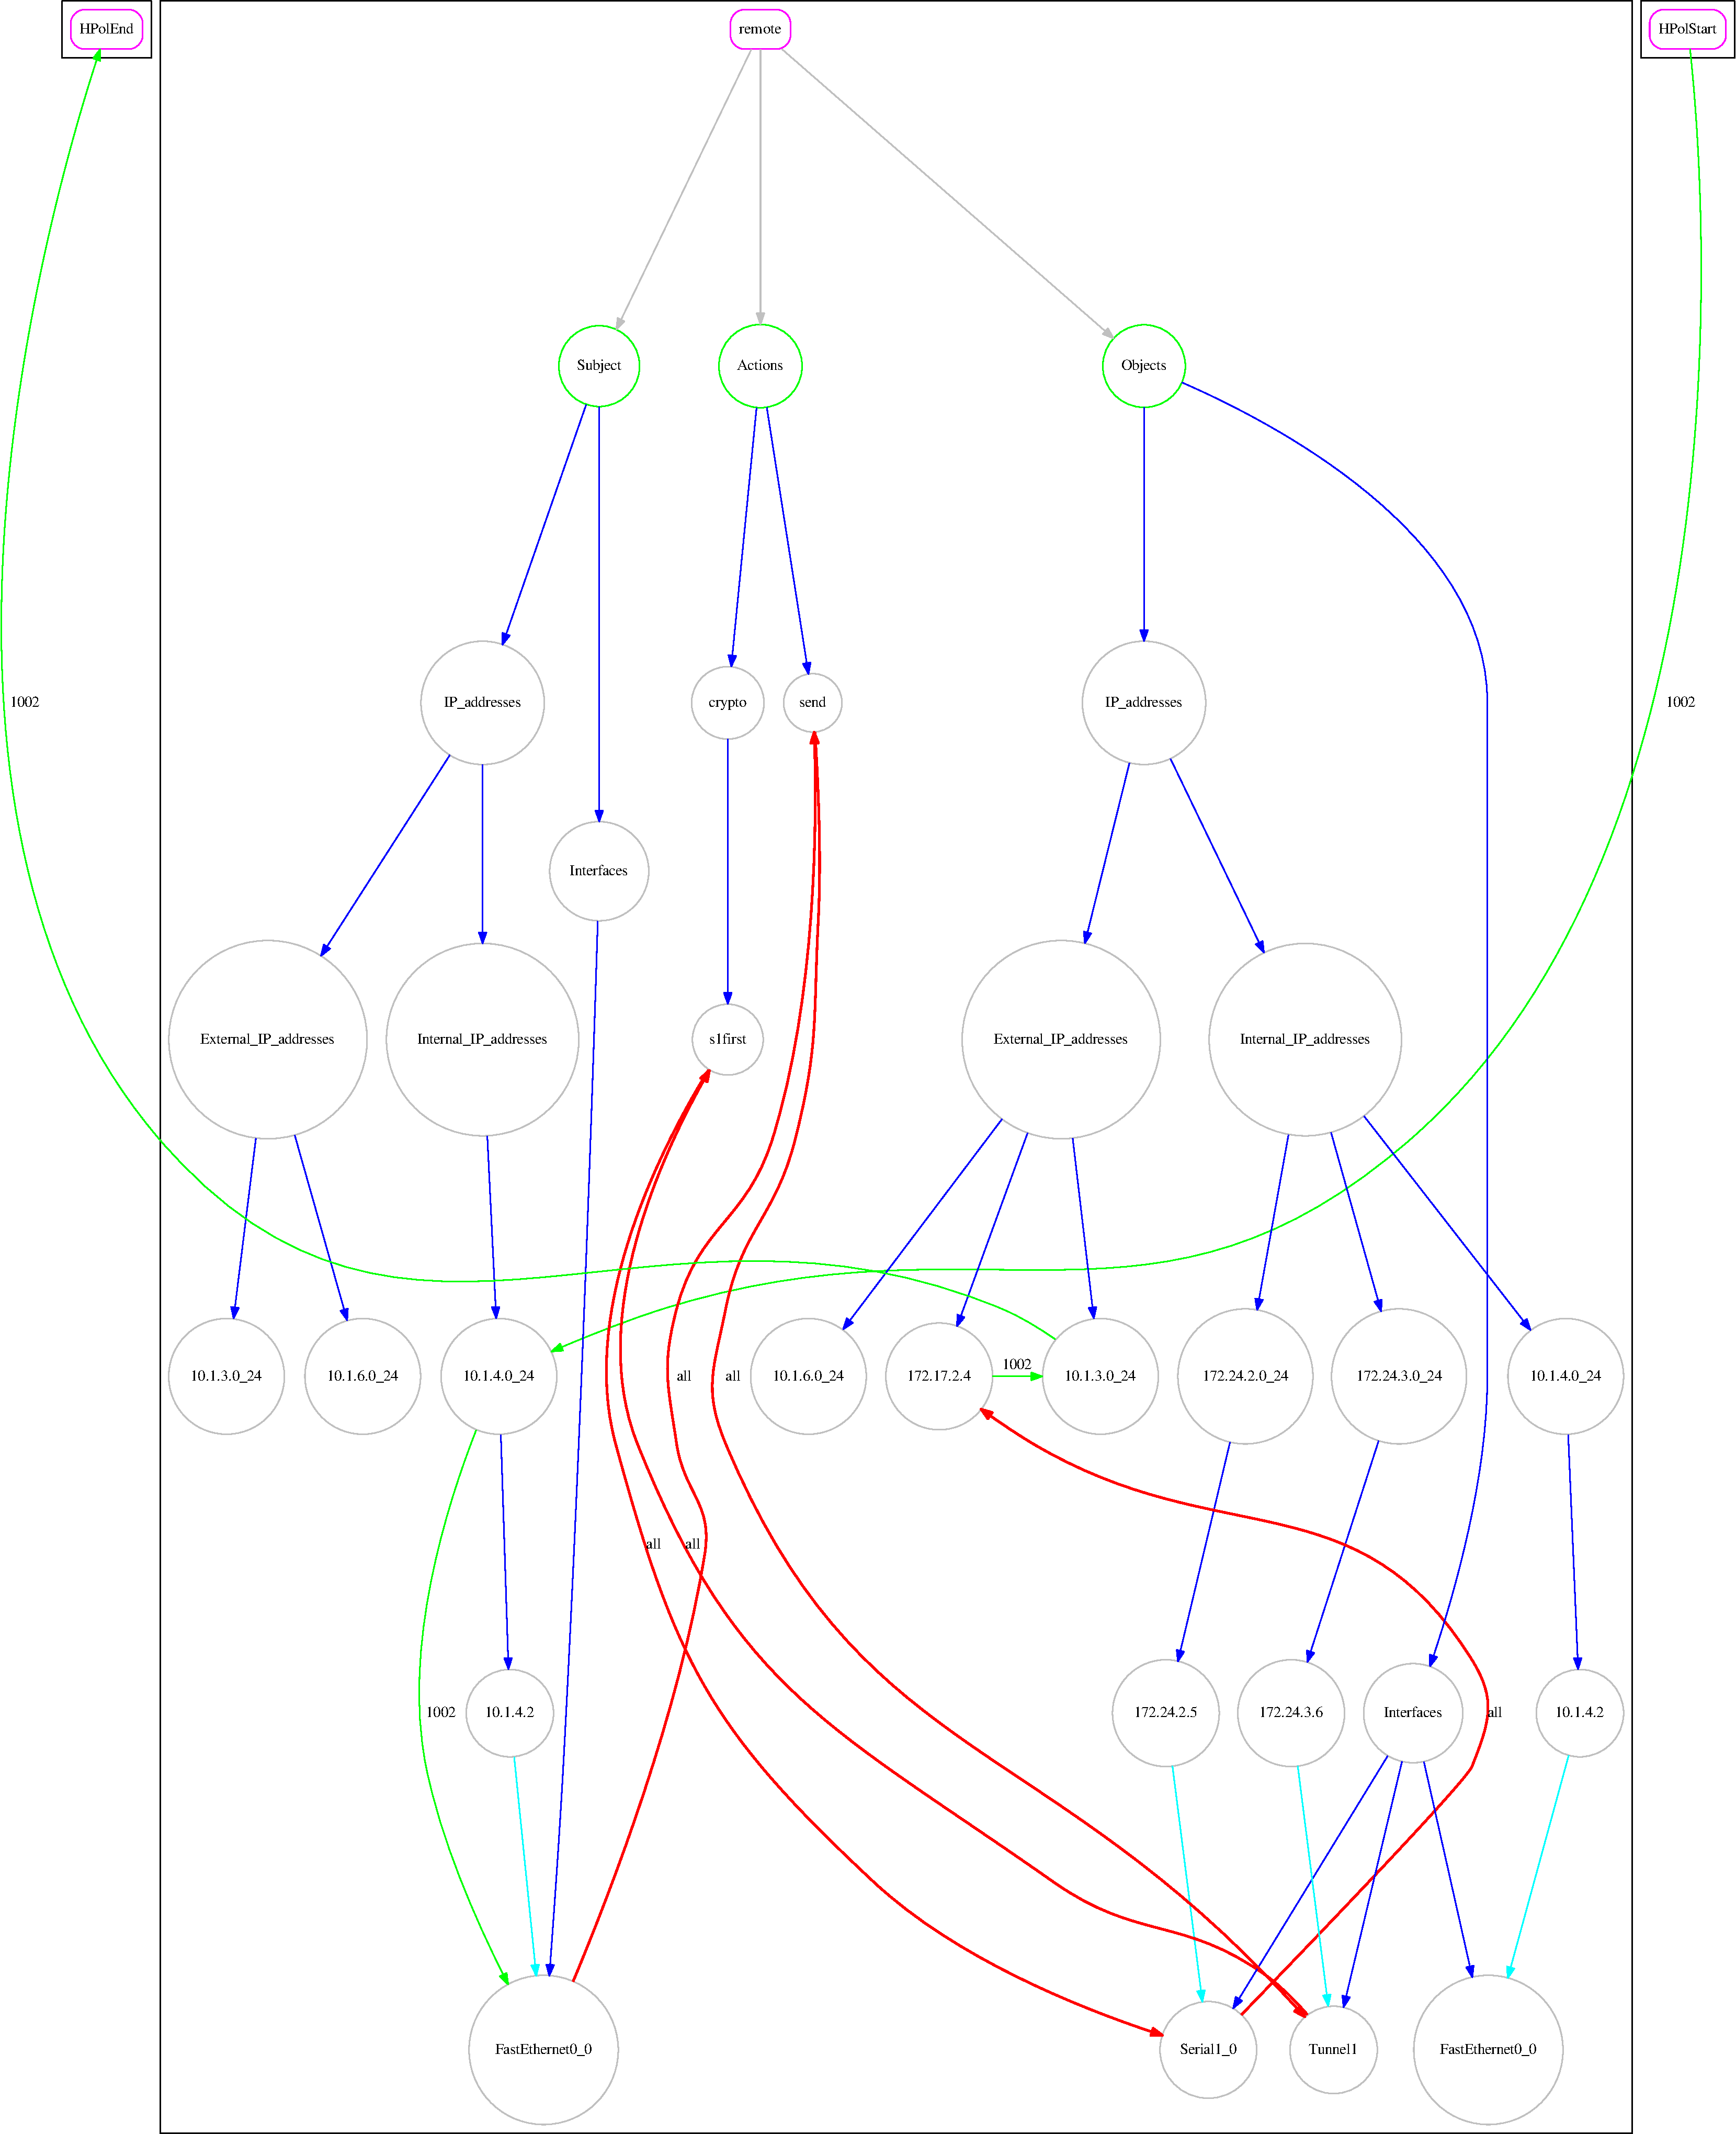
\includegraphics[angle=90, height=.9\textheight, width=\textwidth]{1002only.pdf}
	\caption[Cisco VPN HPol Policy Model (1002 only)]{Cisco VPN HPol Policy Model: Graph View for Right Router showing only policy 1002}
	\label{Figure:1002Only}
\end{figure*}

%\section{Conclusions}

%{In this research, the first iteration of \ac{hpol} is developed. \ac{hpol} is a formal and hierarchical security policy model and associated tool-set whose goal is to enable the verification of the adherence of low-level, as implemented, security policies with respect to intended and high-level organizational security policy.}

%{\ac{hpol} enables the creation of hierarchical system security policies starting from actual device or application implemented policies. Then, by applying formal policy abstraction steps, the model is able to elevate the low-level security policies into higher-level policies, without information loss. Another formal operation, policy concatenation, enables the construction of more complex system policies from the policies implemented by each of the system components. In addition, the \ac{hpol} tool-set enables the visualization of system security policies in order to aid security analysts with navigating and evaluating system policies.}

%Take this out:
%\paragraph{Formal Model and Policy Operations: }{In this research, we created, in addition to the \ac{hpol} formal model, two novel formal operations for hierarchical security policies: (a) abstraction and (b) concatenation. We believe that additional fundamental research is needed in order to investigate which other formal operations would be needed in order to be able to build complete hierarchical system security policies starting from the low-level device policies, for all types of devices. For example, how can we compose the policies from two firewalls or two SELinux devices belonging to the same overall system of systems. Two operations that we envision we could analyze in the future are (i) merging and (ii) composition. With respect to the \ac{hpol} formal model, as mentioned earlier, we believe that the \ac{hpol} model acts almost as a hierarchically-organized state machine. We would like to further investigate the development of such a formal structure and its ability to not just abstractly model policy but enable the construction of policy model checkers for systems of systems policies.}


%Chapter

\chapter{Applied Formal Policy Verification}
\label{Chapter:PolicyQuerying}

If a system administrator wanted to check if a policy is in effect he or she would have to manually check each node of the network. After checking the network the administrator would have to check the computers the policy applies to as well. This is an inefficient use of a system administrator's time and should be augmented with a framework. %%Framwork?? maybe a better word
\ac{hpol} can parse the configuration files of various components in a network and prepare the data in such a way that a system administrator can write queries to gain information about the current state of the network. 

%In order for \ac{hpol} to function as it does many different pieces need to work together. Parsers are needed to extract the information from various devices. Next the data needs to be transformed into an intermediate language to allow it to be transfered to a knowledge base. Finally, the knowledge base is interpreted and queries are prepared for the interpreter. We choose \ac{hermes} to be used as the intermediate language. \ac{hermes} is fully parameterized and flexible making it perfect for this task. Prolog is then used to create and interpret the knowledge base.

%\section{Parsers}
%move to Formal Router Policy Modeling
%more discriptive section title 
%Work on the \ac{hpol} framework started with individual parsers for three different types of configurations, SELinux, Openstack and Cisco routers. These three components were chosen because they represent elements of a typical network environment. These parsers were necessary for the first step of the \ac{hpol} research, to find out if it is even possible to model various components of a network in \ac{hpol}. While the work is ongoing, it has been discovered that it is possible to model both Cisco routers, or routers in general, and the Openstack knowledge base, Keystone. Figure \ref{HPolExample} illustrates the structure of an \ac{hpol} Model graph.

%The primary purpose of the parsers is to prove that a configuration could be modeled with the \ac{hpol} framework. Currently there is work on three different areas of a corporate network. Cisco routers configurations are being modeled to represent routers and managed switches in the network environment. Keystone from Openstack is being used as a template to model knowledge bases. SELinux is being used to represent modeling mandatory access control systems.

%\section{Prolog}
%Prolog is a logic based programming language. In this experiment, Prolog is used for its speed in knowledge base searching. XSB Prolog is chosen for this experiment for a number of reasons. First XSB Prolog is one of the few Prologs that is compiled into machine language making its base functionality much faster than interpreted Prolog. Second XSB has many features that make knowledge base searches faster than other Prolog distributions. Also XSB Prolog is still being developed	meaning known bugs in the language will be removed and new features could arrive with each release \cite{XSB}.

\section{Modifications to HERMES}
As mentioned in chapter \ref{Chapter:Introduction}, the \ac{hermes} language had to enhanced to make it fit for its role in the \ac{hpol} project. While the overall effect of the modification was minor, the \ac{hermes} compiler had to be written to successfully allocate these changes. The changes to the \ac{hermes} language were as follows:
\begin{enumerate}
	\item Modified the lexical analyzer
	\item Added syntax for the following attribute types:
	\begin{enumerate}
		\item Lists
		\item Tuples
		\item List of Tuples, aka Dictionaries
	\end{enumerate}
	\item Added Full parameterization
\end{enumerate}

The lexical analyzer was modified to allow more types of special characters in identifiers. The original \ac{hermes} only allowed identifiers to have the same regular expression as Prolog terms. In \ac{hermes} identifiers are used to identify entry types and names as well as attribute key-value pairs. The original regular expression that defined an identifier is \verb|[A-Za-z][A-Za-z0-9_]*|, which only allows for a very restricted set of possible identifiers. The new lexical analyzer allows for a greater range of symbols in an identifier including dots, hyphens and underscores. The new identifier regular expression is \verb|[A-Za-z0-9][A-Za-z0-9._-]*|. The regular expression was modified to allow for identifiers that take the form of IP address and subnets. The new lexical analyzer can be expanded as needed as well. Because all identifiers are stored in Prolog as strings the number possible of characters is only limited to the size of the ASCII table. However, because we only needed the symbols in the new regular expression this is all that was included.

New attributes were added to allow greater flexibility with \ac{hermes} entries. The original \ac{hermes} compiler only allowed for single-word key value pairs and key string pairs. The new \ac{hermes} parser also allows for list, tuples, and list of tuples, or dictionaries. Listing \ref{Listing:Fullhermes} shows a \ac{hermes} entry that includes all attribute types. Lists were also added to list all nodes in a policy. Tuples and lists of tuples were because they are common data types in languages and can be useful in an unforeseen project.

\begin{lstlisting}%
[
caption=HERMES entry with all types of attributes.,
label=Listing:Fullhermes,
style=hermes,
]
Entry: example
{
	key:value;
	key:"string";
	key:[list, of, values];
	key:(value, tuple);
	key:[(list, of), (value, tuples)];
}
\end{lstlisting}

The last modification to \ac{hermes} was full parameterization. A new compiler was developed to enable true parameterization. The \ac{hermes} language is now truly parameterizable for all identifiers. There are on longer any keywords in the \ac{hermes} language. The only required piece of \ac{hermes} is the general syntax structure.

\section{A Formal Model for Policy Querying}
This section will refer to figure \ref{HPolExample} and the scenario that is modeled by the figure. The scenario for this experiment models the access control of a file system found in a system such as Linux. This model contains a user named \texttt{User\_A}, an action called \texttt{Action\_B} and an object called \texttt{Object\_C}. The names chosen for this experiment are arbitrary but are used to simplify tracing each component throughout this example. In the model there is also a policy with the identifier 1001. Policy 1001 states that \texttt{User\_A} can preform \texttt{Action\_B} on \texttt{Object\_C}. This can be compared to a user named Bob being able to read a file called documents. 


\begin{figure}
	\centering
	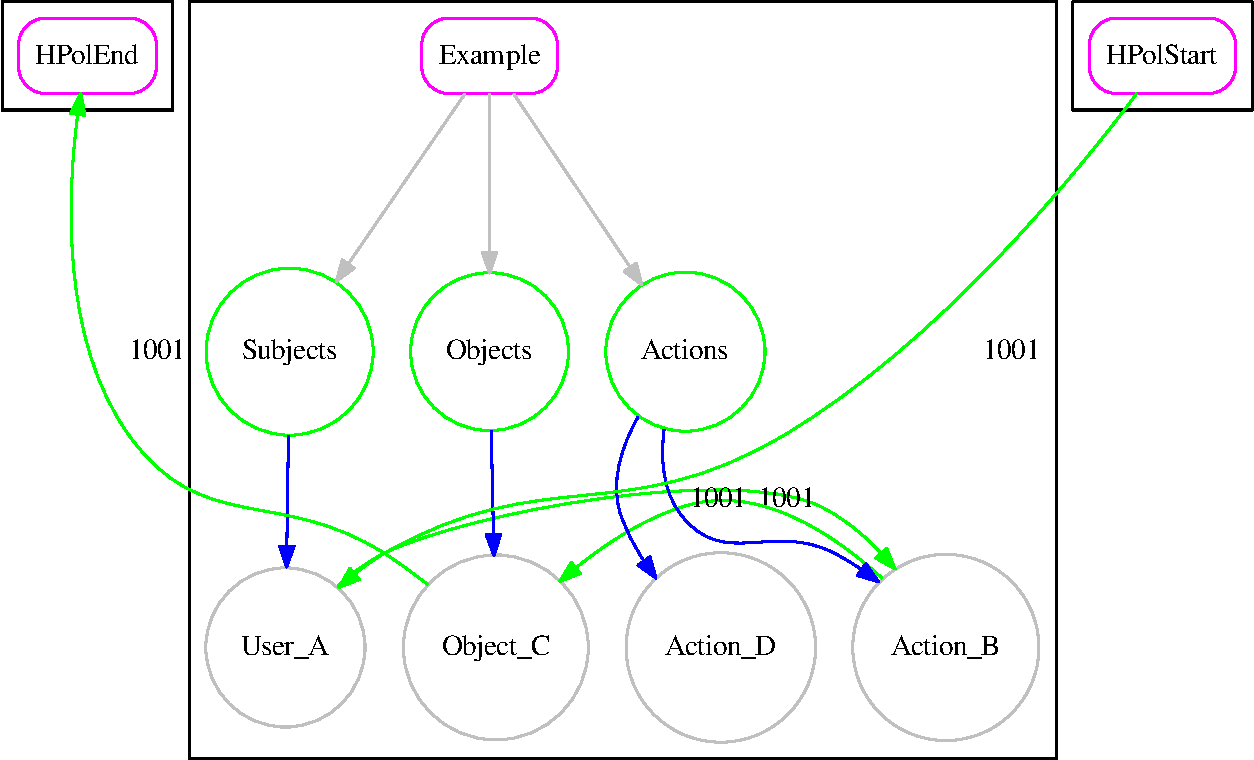
\includegraphics[width=\textwidth]{paper2Example.pdf}
	\caption{Basic Example of a \ac{hpol} Graph.}
	\label{HPolExample}
\end{figure}

Once the structure of the graph and the policies that traverse through the graph have been created, the model needs to be translated into an intermediate language that can be used in the next stage. This is where the \ac{hermes} policy language comes in. Because of its full parameterization and its flexibility as described in section \ref{Section:Hermes}, the \ac{hermes} language is a perfect intermediate step when converting from the \ac{hpol} formal model. By using a series of graph tracing algorithms the structure of the \ac{hpol} model is translated into a series of entries in the \ac{hermes} format. After that the policies of the model are then traced as well and are converted into \ac{hermes} as well. Listing \ref{HERMES_Subject} contains an example of the Subject node in \ac{hermes} form.

\begin{figure*}
	\centering
	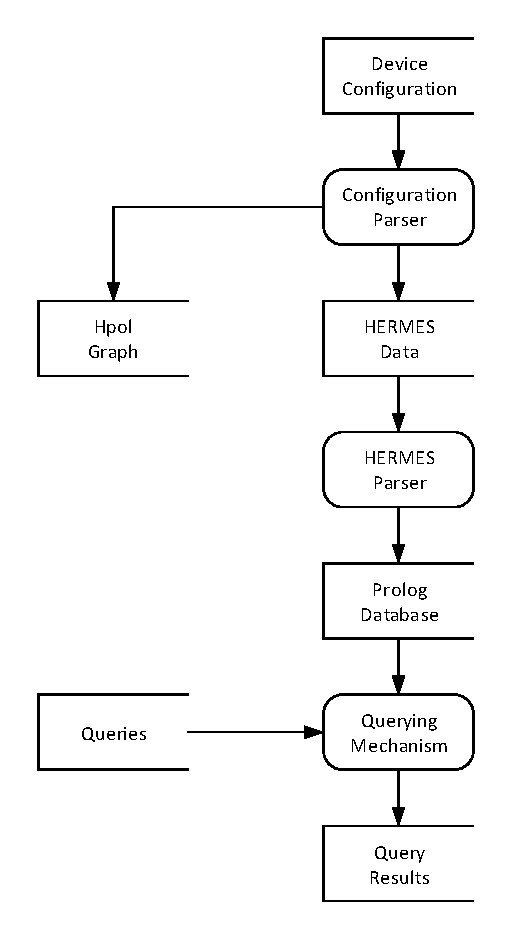
\includegraphics[height=.9\textheight]{ImageV2.pdf}
	\caption[HPol Framework Data Processing Flowchart]{Data flow diagram showing the processing of the data from system configuration to query mechanism.}
	\label{BigPicture}		
\end{figure*}	

Figure \ref{BigPicture} is data flow representation of how data is processed in the \ac{hpol} framework. Data starts as device configuration files. This data is run through a custom configuration parser for each type of device. The output of this parser is \ac{hermes} data and a visual representation of the \ac{hpol} Graph. This transformation can be seen in figure \ref{Cisco_Hermes_1}. An example of the \ac{hpol} graph can be seen in figure \ref{HPolExample}. Next the data is run through the \ac{hermes} parser where it is turned into a Prolog knowledge-base. Listing \ref{Prolog_example1} contains an example snippet of the created Prolog knowledge-base. Simultaneously, queries are created in \ac{hermes} and are fed into the querying mechanism to produce results. Listings \ref{HERMES_query1} and \ref{HERMES_query2} show queries written in HERMES and \ref{XSB_example_result} the results of the queries.


\begin{lstlisting}%%
[
caption = {Subject node written out in HERMES.},
label = {HERMES_Subject},
style=hermes,
float
]
SubDomain:Subjects
{
	Description: "Subjects";
	Path: "Example/Subjects";
	Type: Subjects;
	Children: ["User_A"];
}
\end{lstlisting}

As listing \ref{HERMES_Subject} shows, each node and policy in an \ac{hpol} model is contained in a \ac{hermes} entry. This entry is composed of two parts, a header and a body. The header of an entry contains the type of the entry and the name of the entry separated by a colon. In listing \ref{HERMES_Subject} there exists a \ac{hermes} entry with the type \texttt{SubDomain} called \texttt{Subject}. All descendants of type \texttt{SubDomain} are of type \texttt{Node}. The domain and sub domain keywords are used to identify the root of the graph and its direct children.  The body of an entry resides in curly braces. Inside the curly braces exists the properties of the graph. Properties in \ac{hermes} have a key value pair that are separated by a colon. Every property entry that is formed from by the \ac{hpol} model will have the entries \texttt{Description}, \texttt{Path}, \texttt{Type}, and \texttt{Children}. The \texttt{Description} entry is the name of the node reiterated as a string so invalid characters can be used. The \texttt{Path} entry is the path of the given node starting at the root of the tree. Currently this field has no purpose and might be removed. The \texttt{Type} entry states the node's type. Finally, the \texttt{Children} entry identifies the children of the node. As seen in the graph this nodes path is \texttt{Example/Subject} and the only child of this node is \texttt{User\_A}. All of this information will be extremely useful when it is time to reconstruct the graph from the \ac{hermes} source.

\begin{lstlisting}%%
[
caption={HERMES form of Policy 1001.},
label={HERMES_1001},
style=hermes,
float
]
Policy: 1001
{
	Description: "HPol Policy";
	Status: Enabled;
	Path: [HPolStart, User_A, Action_B, Object_C, HPolEnd]
}
\end{lstlisting}

\section{Policy Specification in HERMES}
Polices are also modeled with the \ac{hermes} language. Listing \ref{HERMES_1001} shows the \ac{hermes} form of Policy 1001. As listing \ref{HERMES_1001} shows, policies are contained by the same type of entry as nodes are. There are, however, some differences. The entry-type and identifier syntax are still present as required by the \ac{hermes} syntax, but the properties of the entries are altered. Instead of \texttt{Type} and \texttt{Children} entries, there is now \texttt{Order}. Also, Path has a different meaning when referring to a policy. When a policy is represented in \ac{hermes}, \texttt{Path} is the path the policy takes through the graph and \texttt{Order} is the order of the graph nodes in the policy. There is also a status entry present. This states whether or not the policy should be active. When being generated from configuration files, all polices will receive the active status because the parsers can only find active polices. The \texttt{Path} entry contains a list of tuples. These tuples are type ID pairs for the nodes that are relevant to the path. The \texttt{Order} key also has a value of a list of tuples. These tuples contain order ID pairs to identify the place of a node in the policy.

\section{Formal Query Structure in HERMES}
Queries are also created in the \ac{hermes} format. Currently, queries enable asking allow and disallow questions. For example, if a systems administrator wanted to know if \texttt{User\_A} could preform \texttt{Action\_B} on \texttt{Object\_C}, the query would look like listing \ref{HERMES_query1}. This query contains three major parts. First, the type of the entry is \texttt{Query}. Second, one of the key value pairs is the \texttt{Allow} rule. This states whether the evaluator should be checking if the action is allowed or disallowed in the \ac{hpol} graph. Listing \ref{HERMES_query2} contains an example of a query asking if the user, \texttt{User\_B}, can preform the action, \texttt{Action\textunderscore D} on the object, \texttt{Object\textunderscore C}. While figure \ref{HPolExample} contains an \texttt{Action\textunderscore D} node, there is no policy that allows \texttt{User\textunderscore A} to preform \texttt{Action\textunderscore D}. Being able to make this distinction is a crucial part of the \ac{hpol} framework. A system administrator needs to make sure an action is not possible just as much as he needs to make sure that one is. Finally, the \texttt{Subject}, \texttt{Action}, and \texttt{Object} keys have values that are used as the parameters of the query.


\begin{lstlisting}%%
[
caption={Example is allowed query written in HERMES.},
label={HERMES_query1},
style=hermes,
float
]
Query: 1
{
	Allow: yes;
	Subject: "User_A";
	Action: "Action_B";
	Object: "Object_C";
}
\end{lstlisting}

\begin{lstlisting}%%
[
caption={Example is not allowed query written in HERMES.},
label={HERMES_query2},
style=hermes,
float
]
Query: 2
{
	Allow: no;
	Subject: "User_B";
	Action: "Action_D";
	Object: "Object_C";
}
\end{lstlisting}


Listing \ref{Listing:ContainsQuery} shows a second type of query. This query type only has one keyword in the body section of its entry. This keyword is \texttt{Contains}. The value of \texttt{Contains} is a list containing nodes that are to be found in a policy. The purpose of the \texttt{contains} query is for searching for policies that contains nodes in the order they show up in the list. Every node does not have to be present in a \texttt{Contains} query for a result to be produced. Listing \ref{Listing:ContainsQuery} shows the same nodes in question as listing \ref{HERMES_query1} to show the similarities between the nodes. However, if a security professional just wanted to know a piece of the puzzle such as which polices involve \texttt{Object\_C} then he or she would write a query similar to \ref{Listing:ContainsObjectC}. Also, this form of query does not give regard to the context of the nodes it is searching for, this allows a faster searching through the policies when finding results. 


\begin{lstlisting}%%
[
caption={Query including \texttt{Contains} keyword.},
label={Listing:ContainsQuery},
style=hermes,
float
]
Query:3
{
	Contains:[User_A, Action_B, Object_C];
}
\end{lstlisting}

\begin{lstlisting}%%
[
caption={Query to search for polices containing \texttt{Object\_C}.},
style=hermes,
label={Listing:ContainsObjectC},
float
]
Query:4
{
	Contains:[Object_C];
}
\end{lstlisting}

\section{Loading HPol Formal Models into Prolog}
Once all entries have been created in \ac{hermes}, the data needs to be stored in a Prolog knowledge-base. XSB Prolog is used as the Prolog engine during this process \cite{XSB}. In order to complete this process, a translator is created to convert the \ac{hermes} format files into a Prolog knowledge base. The compiler for this task is written in Prolog as well. For each entry in a \ac{hermes} file, a series of Prolog facts are created. When a new entry is encountered, a new defining fact about the entry is created and is contained in the predicate \texttt{entityDef}. Next each key value pair of an entry is created into a series of facts contained within the predicate \texttt{entityField}. Each entry in \ac{hermes} is given a unique identifier that is composed of the input file name and the identifier it was originally assigned in \ac{hermes}. Listing \ref{Prolog_example1} contains the entire set of Prolog facts stored about the Subject node referred in figure \ref{HPolExample} and listing \ref{HERMES_Subject}.

\begin{figure*}
	\begin{lstlisting}%%
	[
	caption={Prolog facts about the \texttt{Subject} node.},
	label={Prolog_example1},
	style=hermes,
	]
	entityDef(idhermes_out_Subjects, "Subjects", "hermes.out", "SubDomain").
	entityField(idhermes_out_Subjects, "Description", "Subjects").
	entityField(idhermes_out_Subjects, "Path", "Example/Subjects").
	entityField(idhermes_out_Subjects, "Type", "Subjects").
	entityField(idhermes_out_Subjects, "Children", ["User_A"]).
	\end{lstlisting}
\end{figure*}

Because all data needs to be captured in order to recreate the configuration files, there is sometimes more data than needed contained within the Prolog facts. For the \texttt{Subject} node, there are many facts that are generated. First, an \texttt{entityDef} predicate is used to initially declare the existence of the \texttt{Subject} node. Next, \texttt{entityField} predicates are used to define the various fields found in the \ac{hermes} example in listing \ref{HERMES_Subject}. The conversion between \ac{hermes} properties and Prolog facts is one-to-one except in the case when a dictionary is defined in the \ac{hermes}. In this case, each entry of the dictionary is created into its own \texttt{entityField} fact. Both types of predicates use a unique identifier as the first argument of the fact. This unique identifier is used to bind all facts about a given node or policy together.

\begin{lstlisting}%%
[
caption={\texttt{eval\_query} procedure written to evaluate queries.},
label={Listing:EvalQuery},
style=hermes,
float
]
eval_query(ID, Policy):-
	entityDef(ID, _, _, "Query"),
	entityField(ID, "Subject", Subject),
	entityField(ID, "Action", Action),
	entityField(ID, "Object", Object),
	entityField(ID, "Allow", "yes"),
	atom(ID),!,
	policy_containing(Subject, Action, Object, Policy).
\end{lstlisting}

\section{Querying an HPol Formal Model}

Once the Prolog knowledge-base is created, a series of Prolog procedures are created in order to evaluate a query. Listing \ref{Listing:EvalQuery} contains an example of one the procedures used to evaluate queries. Listing \ref{XSB_example_result} contains the results of the two queries in figures \ref{HERMES_query1} and \ref{HERMES_query2}. The first set of results represents the allow query in listing \ref{HERMES_query1}. This result is stating that the query with the identifier \texttt{idquery\_herm\_1} is being satisfied by the policy \texttt{idhermes\_out\_p1001} or policy 1001 from figure \ref{HPolExample}. It is important to note that the identifiers used internally by Prolog are generated at the time of compilation to facts. The original names of the policies and queries are contained in \texttt{entityDef} predicate of the Prolog knowledge base. 

\begin{lstlisting}%%
[
caption={Results of Queries 1 and 2.},
label={XSB_example_result},
style=hermes,
]
| ?- eval_query(QueryName, PolicyName).

QueryName = idquery_herm_1
PolicyName = idhermes_out_p1001;

QueryName = idquery_herm_2
PolicyName = _h180
\end{lstlisting}

The second set of results shows that there are no policies satisfying query \texttt{idquery\_herm\_2}. This is still a positive answer because query 2 is testing to make sure the action is not possible. Because there are no policies that allow the action in question, the query is correct. The \texttt{\_h180} in place of the policy name is Prolog's way of stating that it can not find a valid result for the variable \texttt{PolicyName}.

This section demonstrates that through the use of an example it is possible to model a system and the policies that are in effect in that system. Further, this section illustrates that it is possible to convert the model into a database which can be queried for details about the system. The next section of this thesis demonstrates this concept with a real-world scenario.

\chapter{Case Study: Cisco Router Querying}
\label{Chapter:CiscoPolicyQuerying}
The case study to test whether the \ac{hpol} framework mechanism can model a real world scenario is done on the configurations of a pair of Cisco routers connected by a VPN tunnel. The configuration files of the two routers were parsed and converted into two separate \ac{hpol} models as described in chapter \ref{Chapter:CiscoRouterPolicyModeling}. The model is similar to the \texttt{Subject}, \texttt{Actions}, \texttt{Objects} format as the previous example except that subnets and interface names are placed under the \texttt{Objects} subtree. Also, the send and encryption actions are placed in the \texttt{Actions} subtree. Because subnets can be treated as both subjects and objects, all subnets and interfaces were placed under the \texttt{Objects} subtree. 

\section{Querying LAN Policy}
Policies in this model state which subnets or interfaces can send packets to a given destination, also a subnet or interface name. If encryption is needed, the policies pass through the appropriate encryption nodes to signify that encryption takes place when packets are sent to the destination. The model is designed in a way that only allowed actions are generated as policies in the model. A policy for the Cisco router \ac{hpol} model states which subnets and interfaces can communicate with each other. For example, referring back to figure \ref{CiscoRouterAGraph}: policy 1004 of the headquarter's router starts at the policy start node, \texttt{HPolStart} then makes its way to the \texttt{10.1.3.0\_24} node. Next, policy 1004 goes to the \texttt{FastEthernet0\_0} node then the \texttt{Send} node and makes its way to the \texttt{10.1.6.0\_24} node through the \texttt{FastEthernet0\_1} node. Finally, the policy makes it to the \texttt{HPolEnd} node; this is where all policy paths must end. This policy reads as an IP address from the \texttt{10.1.3.0\_24} subnet can send packets to an IP addresses in the  \texttt{10.1.6.0\_24} subnet. 

Once the \ac{hpol} model has been generated, the model is converted into \ac{hermes}. This action is the same as its counterpart in the previous section. Figure \ref{Cisco_Hermes_1} shows the transition of the Cisco configuration file into the \ac{hermes} representation of the same data. Much of the data from this node is stored in different areas of the model graph. For example the IP address and subnet of this interface is a parent of this node. Data is stored in this manner so other devices that fall under the same subnet can be placed in their proper place without having to copy or recreate data. The result in figure \ref{Cisco_Hermes_1} shows the description of the node as well as the node's path and type. Because of how the path works in the \ac{hpol} model, all forward slashes are replaced with underscores. Each parser contains its own caveats when transforming configurations into \ac{hermes}.  

\begin{figure*}
	\begin{tabular}{ c | c }
		{\begin{lstlisting}%%
			[
			style=hermes,
			frame=none,
			numbers=none,
			tabsize=1
			]
interface FastEthernet0/0
ip address 10.1.3.3 255.255.255.0
no ip directed-broadcast
no keepalive
full-duplex
no cdp enable
		\end{lstlisting}}
		&
		{\begin{lstlisting}%%
			[
			style=hermes,
			frame=none,
			numbers=none,
			tabsize=1
			]
Node: FastEthernet0_0
{
Description: "FastEthernet0_0";
Path: "base/Objects/
...Interfaces/FastEthernet0_0";
Type: object;
}
		\end{lstlisting}}
	\end{tabular}
	\caption[Cisco Configuration to HERMES Processing and Translation Example]{This figure contains the before (left) and after (right) when data is converted from a Cisco router configuration file to a \ac{hermes} entry.}
	\label{Cisco_Hermes_1}
\end{figure*}

Once in \ac{hermes} the data is parsed. The data is then loaded into the Prolog knowledge base and is ready to query. Queries of each type are created to test the system. The first query asks if the \texttt{10.1.3.0\_24} subnet can \texttt{send} to the \texttt{10.1.6.0\_24} subnet. The second query wants to check that the \texttt{10.1.9.0\_24} subnet cannot \texttt{send} to \texttt{10.1.6.0\_24} subnet. Both of these queries return yes as a result. The first query result returns that policy \texttt{idhermes\_out\_p1004}, or policy 1004, satisfies the query. This means that according to the configuration that is parsed, it is possible for a device in the \texttt{10.1.3.0\_24} subnet to send a packet to a device in the \texttt{10.1.6.0\_24} subnet. It is also not possible for a device in the \texttt{10.1.9.0\_24} subnet to \texttt{send} the \texttt{10.1.3.0\_24} subnet. 

\section{Querying Tunnel Policy}	

In chapter \ref{Chapter:CiscoRouterPolicyModeling} policy 1002 was traced with reasoning and evidence for each node chosen. Listing \ref{Listing:1002FullHERMES} shows the \ac{hermes} entry for every node involved with policy 1002 including the \ac{hermes} entry for policy 1002.

\lstinputlisting[
tabsize=2, 
caption=HERMES entries for all nodes associated with policy 1002., 
label=Listing:1002FullHERMES,
style=hermes,
]{listings/HermesExamples.txt}

Referring back to policy 1002, we know that this policy allows the 10.1.4.0/24 subnet to send to the 10.1.3.0/24 subnet through Tunnel1. The listing below shows the query that is required to ask if this is possible:

\begin{lstlisting}[style=hermes,]
Query: 1
{
	Allow: yes;
	Subject: "10.1.4.0_24";
	Action: "send";
	Object: "10.1.3.0_24";
}
\end{lstlisting}

As shown above and in the previous section, the Subject, Action and Object query is used to verify that subnet 10.1.4.0/24 can send to the 10.1.3.0/24 subnet. The listing below shows this query being evaluated in the XSB Prolog interactive shell:

\begin{lstlisting}[style=hermes,]
| ?- eval_query_by_name(1, A).

A = 1002

yes
\end{lstlisting}

In this query example the procedure \texttt{eval\_query\_by\_name} is used to allow a user to evaluate the queries by the name given to the query while in \ac{hermes} form instead of the internal identifier that is used to separate queries from different files with the same name. This procedure also returns the identifier of the policy as it appears in the original \ac{hpol} diagram. As the above listing shows, policy 1002 allows subnet 10.1.4.0/24 can send to subnet 10.1.3.0/24; just as was traced in chapter \ref{Chapter:CiscoRouterPolicyModeling}.

\section{IP to IP Query}
This thesis thus far has covered the process behind router-policy formal modeling and verification, which, in short, is as follows: 

\begin{enumerate}
	\item Model a router configuration file.
	\item Convert the model into \ac{hermes}.
	\item Create queries for the model in \ac{hermes}.
	\item Load both model and queries into Prolog.
	\item Use procedures created for this research to evaluate queries.
\end{enumerate}

This thesis has shown the process is possible for both dummy examples and for real router configurations. However, everything that has been discussed to this point applies to all \ac{hpol} formal models for all devices because the previous query types referred to entities that explicitly existed on an \ac{hpol} model. For example, subnets and interfaces explicitly exist on Cisco router formal models. To round out the research for this thesis, one more procedure was written that applies to only router policy models. Prolog procedures were written that could evaluate whether one IP address can send to another. This query is special because an extra layer of processing is required to evaluate it. 

In the previous sections, queries were discussed regarding whether one subnet can communicate with another; however, individual IP addresses were never used, just subnets. In the IP to IP query, an evaluation is made to determine if source and destination IP addresses belong to subnets that exist in \ac{hpol} router polices. These queries are then evaluated as \texttt{send} queries where the source IP address belongs to the \texttt{Subject} subnet, the action is \texttt{send}, and the destination IP address belongs to the \texttt{Object} subnet. Listing \ref{Listing:IPSendQuery} contains the procedure that is at the center of the IP to IP query evaluator.

\begin{lstlisting}%%
[
style=hermes,
caption={\texttt{ip\_send\_query} procedure of the IP to IP query evaluator},
label={Listing:IPSendQuery},
float
]
ip_send_query(IP1, IP2, Policy):-
	policy_containing(SubjectCodes, "send", ObjectCodes, Policy),
	fmt_write_string(Subject, "%s", args(SubjectCodes)),
	fmt_write_string(Object, "%s", args(ObjectCodes)),
	ipINsub(Subject, IP1),
	ipINsub(Object, IP2).
\end{lstlisting}

In section \ref{Section:HPolPacketTrace} an \ac{hpol} policy was traced to verify that IP 10.1.4.3 could send to IP 10.1.3.6. That policy trace had to start at the subnet level due to limitations of the \ac{hpol} formal model's ability to model routers and the lack of specific device IP address information in the router's configuration. Because of these setbacks, the policy had to trace from subnet 10.1.4.0/24 to subnet 10.1.3.0/24. For this last piece of research, a new type of query and new evaluation procedures were created in Prolog to allow a security specialist to write queries that pertain to individual IP addresses. 

\begin{lstlisting}[
style=hermes,
caption={Final type of query, IP to IP.},
label={Listing:IPtoIPquery},
float
]
Query: 1
{
	Allow: yes;
	Src: 10.1.4.3;
	Dest: 10.1.3.6;
}
\end{lstlisting}

Listing \ref{Listing:IPtoIPquery} contains an example of an IP to IP query. In this query the same basic \ac{hermes} structure remains. However, there is a variation in the key value pairs in this type of query. In this query type there is still the \texttt{Query} keyword for the type of \ac{hermes} entry and the \texttt{Allow} keyword remains. This is where the similarities end. There are now \texttt{Src} and \texttt{Dest} keywords that denote the source and destination IP addresses, respectively. The source and destination IP addresses in this query are 10.1.4.3 and 10.1.3.6, which are the same IP addresses being verified in section \ref{Section:HPolPacketTrace}'s policy trace.

\begin{lstlisting}[
style=hermes,
caption={Result of the IP to IP query.},
label={Listing:IPtoIPqueryResult},
float
]
| ?- eval_query_by_name(1, A).

A = 1002

yes
\end{lstlisting}

Listing \ref{Listing:IPtoIPqueryResult} shows the result of the IP to IP query. The policy that was returned in this query was policy 1002, the same policy traced in section \ref{Section:HPolPacketTrace} manually. This final type of query is significant because it demonstrates that the \ac{hpol} formal model and the related framework can parse the configuration of a (Cisco) router and have the results semi-automatically verified through the use of queries. This provides security personnel a more refined way of determining if router configurations comply to the policies that are meant to define them.


\section{Performance}
Converting the Cisco \ac{hermes} output from the \ac{hpol} model into a Prolog knowledge base takes about 5 seconds running XSB Prolog in single core mode with a 2.00 GHz computer running with 12 GB of RAM. However when running the XSB process takes less than 50 MB of RAM. Once the \ac{hermes} data is converted into a Prolog knowledge base and loaded, it takes a negligible amount of time to evaluate each query. Fortunately, unless the \ac{hermes} data changes, it only needs to be converted once.

\section{Discussion}
The results of the queries demonstrate it is possible to successfully query the configuration of a network component such as a Cisco router. For both allow and deny queries, the Prolog query system can identify queries and all policies that satisfy any given query. The system can also take a query identifier as an argument and return all policies that satisfy the query. It has also been discovered due to the nature of Prolog that the reverse is acceptable; a policy can be given and all queries that the policy satisfy will be returned.

In this chapter three examples of a case study were presented where the \ac{hpol} formal models of two Cisco routers were queried. For both the LAN query and the tunnel query, accurate results were produced. In the final example, it was shown queries that allow the verification of IP address communication can be used to further verify the correctness of router policies.

\chapter{Future Work}
\label{Chapter:FutureWork}

The \ac{hpol} framework is still within its infancy. There are many different components that need to be combined or created in order for it to reach its full potential. Parsers need to be generated for additional types of devices such as firewalls and managed switches. Policy concatenation also needs to be implemented. This will allow queries to be generated across a variety of components of an enterprise network. The ability to configure components through \ac{hpol} also needs to be implemented. Finally, a GUI should be set up to graphically organize all of the data presented by an \ac{hpol} policy.

\section{Additional Device Configuration Parsers}
In order to prove \ac{hpol}'s flexibility, parsers need to first be created for every type of component found in an enterprise network. Firewalls and managed switches are a large part of the networking side of an enterprise network. File system access control is another field that needs to be researched to increase \ac{hpol}'s flexibility. Once these components have \ac{hpol} parsers, the model for each type can be formalized. Next the different brands and models would have to have parses created for them to match the model created for the general component template.

\section{Formal Policy Concatenation}
In order for \ac{hpol} to evaluate an enterprise network as a whole policy, models have to be linked together. The hypothesis is that if the start and end nodes of multiple policies are connected, then it is possible to query a policy on a larger scale. For example, if two router policies are linked together, then it is possible to query whether an IP address in subnet X on router A can send a packet to the IP address of a subnet in router B. However, it is not possible to determine if the policy is correct when looking at each router's configuration separately. When looking at Router B's configuration in isolation, it is only possible to determine whether router A can send packets to a subnet in router B. By look at only this configuration, there is no way of knowing the origin of the packet from router A. Furthermore, when looking at router A's configuration separately, it can be seen that an IP in subnet X can send a packet to router B. This, however, is still not enough information to determine whether the policy is in effect. Only when the two models are combined is it possible to see that packets from a specific IP address in a subnet of router A can be sent to one of router B's subnets. This is enough information to determine that the policy is correct.

For example, figures {\ref{CiscoRouterAGraph}} and {\ref{CiscoRouterBGraph}} show the policy graphs for the two routers used in the given VPN configuration. However, the overall system policy for this VPN Tunnel cannot be observed by analyzing the configurations of the two routers separately.

{In order to be able to analyze a network tunnel system policy in a holistic way, a complex system security policies needs to be built starting from the policies of the composing components of the system. The \ac{hpol} formal model enables this by the introduction of the concatenation of security policies formal operation. The Cisco VPN Tunnel policy model is used to demonstrate this operation.}

{By superimposing the {\textsl{End}} node in the {\textsl{hq-sanjose}} (Left) router to the {\textsl{Start}} node in the {\textsl{ro-rtp}} (Right) router, a system wide and formal network policy that models the complete VPN Tunnel configuration is created.}

{This formal Policy Concatenation Operation, in conjunction with other additional operations, would enable the formal construction and analysis of system-wide and holistic security policies. In this case, the visualization and analysis of the complete VPN Tunnel system policy is possible by concatenating the policies of the two integrating routers.}

While formal policy concatenation operations seem trivial, there is a greater more complex problem in this operation. Currently, \ac{hpol} formal models have no since of self and are unable to identify themselves in another model. Once \ac{hpol} models are able to identify themselves in other models then policy concatenation can be implemented. 

\section{Policy-Based Device Configuring}
Once parsing and policy concatenation are implemented, policy-based configuration functionality can be developed. This functionality enables a system administrator to state a policy and have the \ac{hpol} framework evaluate that policy, determine which configurations need to be changed to place the policy in effect, and then apply the changes to the configurations. This functionality is critical to the \ac{hpol} model. When configurations are parsed, every detail from the old configurations needs to be saved in order to create the new configurations based on both old and newly assigned policies.

%Chapter
\chapter{Summary and Conclusions}
\label{Chapter:SummaryAndConclustions}

In this thesis, the process involved in converting a Cisco router configuration into an \ac{hpol} formal model has been demonstrated. Also introduced was policy querying of an \ac{hpol} formal model with evidence provided using both an example and a case study.

%%%%check this
When converting a Cisco router policy to an HPol formal model there are some key elements. First, all subnets and interface names are placed under the \node{Objects} DAG. Any node that can also act as the subject of a policy is then duplicated under the \texttt{Subjects} DAG. Second, the \node{send} node and all encryption types are placed under the \node{Actions} DAG. Finally, all policies in this model begin with either a subnet or interface node continue to a send or an encryption node and finish at an interface or subnet node. 

Policy queries can be broken down into easy steps. First, all \ac{hpol} models are converted to the \ac{hermes} language. Second, once in \ac{hermes}, the data is read into a Prolog knowledge base. Also part of the second set, queries about the model are written in \ac{hermes} and are loaded into the Prolog knowledge base. Finally, Prolog evaluates the queries with the help of some procedures written for this project.

Both of these operations are described in this thesis using simple examples and Cisco Router configurations. The conclusion of these operations is that it is possible to both model Cisco routers, or routers in general, and then query those models for information about the router's configuration.

Through the use of the \ac{hpol} formal model and the associated framework, security personnel also have the ability to verify the correctness of a Cisco router's configuration. The IP to IP query enables security personnel to write queries for specific IP addresses to further increase the granularity of router policy correctness verification.

Modeling and querying different types of devices is important in industry because system administrators need to be able to know the current status of devices without having to go out and collect and analyze the data manually. A modeling system such as \ac{hpol} can shift the responsibilities of system administrators from worrying about configuring devices correctly to worrying more about the policies that the configurations enforce.


%%%%%%%%%%%%%%%%%%%%%%%%%
\pagebreak

%References
\bibliographystyle{plain}
\addcontentsline{toc}{chapter}{References}
\renewcommand\bibname{References}
\bibliography{paper2,HPolReportBib,fullbibfile}
%Relabels bibliography title as "References"

%\begin{thebibliography}{9} % Sets reference indenting to even with title
%Gives invariant reference tag to particular referece, use ~\cite{Each Author's Last Initial}
%\bibitem{Each Author's Last Initial}
%Name, Journal Name {\bf Volume} (Year) page
%Another Example
%\bibitem{TMO1}
%M. Taketani, S. Machida, and S. Onuma, Prog. Theor. Phys (Kyoto) {\bf 7} (1952) 45.
%\end{thebibliography}

%\pagebreak
%\addcontentsline{toc}{chapter}{Appendix A: HPol Cisco Configuration Parser}
%\section*{Appendix A: HPol Cisco Configuration Parser}
%\lstinputlisting[
%language=python, 
%tabsize=2, 
%style=code,
%]{listings/HPolciscoparser.py}

%Appendix B
%\addcontentsline{toc}{chapter}{Appendix B: Name}
%\section*{Appendix B: Name}
%\ \ \ \ \ The \ldots

%\subsection*{Appendix B.1. Name}
%\ \ \ \ \ The \ldots

%\subsubsection*{Appendix B.1.1. Name}
%\ \ \ \ \ The \ldots

%\subsubsection*{Appendix B.1.2. Name}
%\ \ \ \ \ The \ldots

%\subsubsection*{Appendix B.1.3. Name}
%\ \ \ \ \ The \ldots

%\subsection*{Appendix B.2. Name}
%\ \ \ \ \ The \ldots



\end{document}
